% ****** Start of file apssamp.tex ******
%
%   This file is part of the APS files in the REVTeX 4.1 distribution.
%   Version 4.1r of REVTeX, August 2010
%
%   Copyright (c) 2009, 2010 The American Physical Society.
%
%   See the REVTeX 4 README file for restrictions and more information.
%
% TeX'ing this file requires that you have AMS-LaTeX 2.0 installed
% as well as the rest of the prerequisites for REVTeX 4.1
%
% See the REVTeX 4 README file
% It also requires running BibTeX. The commands are as follows:
%
%  1)  latex apssamp.tex
%  2)  bibtex apssamp
%  3)  latex apssamp.tex
%  4)  latex apssamp.tex
%
\documentclass[%
 reprint,	
%superscriptaddress,
%groupedaddress,
%unsortedaddress,
%runinaddress,
%frontmatterverbose, 
%preprint,
%showpacs,preprintnumbers,
%nofootinbib,
%nobibnotes,
%bibnotes,
 amsmath,amssymb,
 aps,
 prc,
%prb,
%rmp,
%prstab,
%prstper,
%floatfix,
]{revtex4-1}

\usepackage{graphicx}% Include figure files
\usepackage{dcolumn}% Align table columns on decimal point
\usepackage{bm}% bold math
\usepackage{url}
\usepackage{lipsum}
\usepackage{color}
\usepackage{hyperref}% add hypertext capabilities
\usepackage[mathlines]{lineno}% Enable numbering of text and display math
\linenumbers\relax % Commence numbering lines

%\usepackage[showframe,%Uncomment any one of the following lines to test 
%%scale=0.7, marginratio={1:1, 2:3}, ignoreall,% default settings
%%text={7in,10in},centering,
%%margin=1.5in,
%%total={6.5in,8.75in}, top=1.2in, left=0.9in, includefoot,
%%height=10in,a5paper,hmargin={3cm,0.8in},
%]{geometry}

\begin{document}

\preprint{APS/123-QED}

\title{Centrality and transverse momentum dependence of $D^0$-meson production at mid-rapidity in Au + Au collisions at $\sqrt{s_{_{\rm NN}}}$ = 200\,GeV}% Force line breaks with \\
%\thanks{A footnote to the article title}%

%\author{Ann Author}
% \altaffiliation[Also at ]{Physics Department, XYZ University.}%Lines break automatically or can be forced with \\
%\author{Second Author}%
% \email{Second.Author@institution.edu}
%\affiliation%

\collaboration{STAR Collaboration}
\noaffiliation

\date{\today}% It is always \today, today,
             %  but any date may be explicitly specified

\begin{abstract}
  We report a new measurement of $D^0$-meson production at mid-rapidity ($|y|<$1) in Au + Au collisions at $\sqrt{s_{_{\rm NN}}}$ = 200\,GeV utilizing the Heavy Flavor Tracker, the high resolution silicon detector at the STAR experiment. %$D^0$-mesons are reconstructed in their hadronic decay channel $D^0\rightarrow K^-+\pi^+$ and its charge conjugate through topological reconstruction of $D^0$ decay vertices. 
  Invariant yields of $D^0$-mesons in the transverse momentum ($p_{\rm T}$) region of 0--$\sim$9\,GeV/$c$ are reported in various centrality bins. Blast-Wave thermal models are fit to $D^0$-meson $p_{\rm T}$ spectra to study $D^0$ hadron freeze-out properties and radial flow collectivity. The average radial flow velocity extracted from the fit is considerably smaller compared to that of light hadrons ($\pi,K,p$), but comparable to that of multi-strangeness hadrons ($\phi,\Xi^-$), indicating $D^0$ mesons kinetically decouple from the system earlier than light hadrons. Nuclear modification factors ($R_{\rm CP}$ and $R_{\rm AA}$) in various centrality bins are calculated. $R_{\rm CP}$ at $p_{\rm T}>4$\,GeV/$c$ in central 0--10\% Au+Au collisions is significantly suppressed and comparable to that of other light hadrons, re-affirming that charm quarks suffer large amount of energy loss in the hot QCD medium. $R_{\rm CP}$ at low $p_{\rm T}$ is higher than that of light hadrons and shows a characteristic structure consistent with the expectation from model predictions that charm quarks gain sizable collectivity during the medium evolution. %Measured $R_{\rm CP}$ and $R_{\rm AA}$ are compared to several phenomenological model calculations. %These models, tuned to reproduce previous $R_{\rm AA}$ and $v_2$ measurements at RHIC, show nice agreements with our new experimental data in $R_{\rm CP}$ but have some discrepancy for the new $R_{\rm AA}$. 
The new improved measurements are expected to further constrain parameters and reduce their uncertainties in model calculations.

%\begin{description}
%\item[Usage]
%Secondary publications and information retrieval purposes.
%\item[PACS numbers]
%May be entered using the \verb+\pacs{#1}+ command.
%\item[Structure]
%You may use the \texttt{description} environment to structure your abstract; use the optional argument of the \verb+\item+ command to give the category of each item. 
%\end{description}
\end{abstract}

\pacs{25.75.-q, 25.75.Cj}% PACS, the Physics and Astronomy
                             % Classification Scheme.
%\keywords{Suggested keywords}%Use showkeys class option if keyword
                              %display desired
\maketitle
% * <xdong@lbl.gov> 2017-02-14T23:51:52.300Z:
%
% ^.
%\tableofcontents
% * <xdong@lbl.gov> 2017-05-03T17:23:03.215Z:
%
% ^.
% * <xdong@lbl.gov> 2017-05-03T17:23:01.211Z:
%
% ^.

% Chapter one
\section{\label{sec:introduction}Introduction}
The heavy ion program at the Relativistic Heavy Ion Collider (RHIC) and Large Hadron Collider (LHC) studies Quantum Chromodynamics (QCD) at high temperature and density. Over the last decades, experimental results from RHIC and LHC using light flavor probes have demonstrated that a strongly-coupled Quark-Gluon Plasma (sQGP) is created in these heavy-ion collisions. The most significant evidence comes from the strong collective flow and the large high transverse momentum ($p_{\rm T}$) suppression in central collisions for various observed hadrons including multi-strangeness hadrons $\phi$ and $\Omega$~\cite{StarWhitePaper,PhenixWhitePaper,LhcSummary,Adamczyk:2015ukd,Abelev:2014pua}.

Heavy quarks ($c$,$b$) are created predominantly through initial hard scatterings due to their large masses~\cite{Ziwei_Lin,Cacciari}. The modification to their production in transverse momentum due to energy loss and radial flow and in azimuth due to anisotropic flows is sensitive to heavy quark dynamics in the partonic sQGP phase~\cite{Moore}. Recent measurements of high-$p_{\rm T}$ $D$-meson production at RHIC and LHC show a strong suppression in the central heavy-ion collisions. The nuclear modification factor $R_{\rm AA}$, the ratio between the yield in heavy-ion collisions and the number-of-binary-collisions scaled yield in $p+p$ collisions, is used to quantify its level~\cite{Alice_D_RAA_1,Alice_D_RAA_2,CMS_D_RAA_5TeV,Star_D_RAA}. The suppression is similar to that of light hadrons at $p_{\rm T}>$ 4\,GeV/$c$, suggesting significant energy loss for charm quarks inside the sQGP medium. The measured $D$-meson anisotropic flow show that $D$-mesons also exhibit significant elliptic and triangular flow at RHIC and LHC~\cite{Alice_D_v2_276TeV_PRL,Alice_D_v2_276TeV_PRC,CMS_D_vn_5TeV,Star_D_v2}. The magnitude when scaled with the transverse kinetic energy is similar to that of light and strange flavor hadrons. This indicates that charm quarks may have reached thermal equilibrium in these collisions at RHIC and LHC.

In this article, we report measurements of the centrality dependence of $D^0$-meson transverse momentum spectra at mid-rapidity ($|y|<1$) in Au+Au collisions at $\sqrt{s_{_{\rm NN}}} = 200$\,GeV. The measurements are conducted at the Solenoidal Tracker At RHIC (STAR) experiment utilizing the high resolution silicon detector, the Heavy Flavor Tracker (HFT). The paper is organized in the following order: In Section II, we describe the detector setup and dataset used in this analysis. In Section III, we present the topological reconstruction of $D^0$ mesons in the Au+Au collision data, followed by Section IV and V for details on efficiency corrections and systematic uncertainties. We present our measurement results and physics discussions in Section VI. Finally, we end the paper with a summary in Section VII.

% Chapter two
\section{\label{sec:dataset}Experimental setup and Dataset}
The dataset used in this analysis consists of Au + Au collision events at $\sqrt{s_{_{\rm NN}}}$ = 200\,GeV collected by the STAR detector at RHIC in the 2014 year run. The major detectors used in this analysis are the Time Projection Chamber (TPC), the Heavy Flavor Tracker (HFT) detector, the Time of Flight (TOF) detector and the trigger detector Vertex Position Detector (VPD). 

\subsection{\label{sec:dataset:tpctof}TPC and TOF}
The TPC and HFT detectors are the main tracking detectors used in this analysis, while the TPC and TOF detectors provide particle identification for stable hadrons. The TPC and TOF detectors cover the full azimuth and pseudorapidity range $|\eta|<1$~\cite{TPC,TOF}. They have been extensively used in many previous STAR measurements. The TPC provides tracking and momentum measurements for charged particles. Particle identification in this analysis is performed via a combination of the ionization energy loss ($dE/dx$) measured in the TPC and the time-of-flight ($tof$) measured in the TOF with the event start time provided by the VPD detector. The HFT detector provides measured points of high precision that are used to extend the track trajectory and provide high pointing resolution to the vicinity of the event vertex.

\subsection{\label{sec:dataset:trigger}Trigger and Dataset}
The minimum bias trigger used in this analysis is defined as a coincidence between the east and west VPD detectors located at 4.4 $<$ $|\eta|$ $<$ 4.9~\cite{VPD}. Each VPD detector is an assembly of nineteen small detectors with each consisting of a Pb converter followed by a fast, plastic scintillator read out by a photomultiplier tube. To efficiently sample the collision events in the center of HFT acceptance, an online collision vertex along the beam line (calculated via the time difference between east and west VPD detectors) cut of $|V_z^{\rm VPD}|<6$ cm is applied. The coincidence probability in VPD detectors decreases and the online VPD vertex resolution degrades in peripheral events, which have low multiplicity. These introduce some amount of inefficiency for peripheral events in this minimum bias trigger. The correction and centrality selection will be discussed in the next subsection.

\subsection{\label{sec:dataset:Centrality}Trigger Efficiency and Centrality Selection}
Events used in this analysis are recorded with
% the IST and the PXL, 
the reconstructed collision vertex (Primary Vertex, $V_{z}^{\rm TPC}$) within 6 cm of the TPC and HFT centers along the beam direction to ensure uniform and large acceptance. The total drift time of ionization electrons inside the TPC from one end to the other is about 40\,$\mu s$ while the hadronic Au+Au collision rate is typically around 40\,kHz when this dataset is recorded. There is a finite chance that more than one event is recorded in the TPC readout event frame. The VPD is a fast detector which can separate events from different bunch crossings (one bunch cross at RHIC is 106\,$ns$). In order to suppress the chance of selecting the wrong vertex from collisions in bunch crossings different from that of the trigger, the difference between the event vertex $z$ coordinate $V_{z}^{\rm TPC}$ and the $V_{z}^{\rm VPD}$ is required to be less than 3 cm. Approximately 900 M 0-80\% centrality minimum bias triggered events passed these selection criteria and are used in the measurement reported in this paper.

The centrality is selected using the measured charged global track multiplicity $N_{\rm ch}^{\rm raw}$ at midrapidity within $|\eta|$ $<$ 0.5 and corrected for the online VPD triggering inefficiency using a Monte Carlo (MC) Glauber simulation. 0-X\% centrality is defined as the 0-X\% most central in terms of total hadronic cross section determined by the impact parameter between two colliding nuclei. In this analysis, the dependence of $N_{\rm ch}^{\rm raw}$ on the collision vertex position and the beam luminosity has been take into account. The measured track multiplicity distribution from Au + Au 200\,GeV from RHIC run 2014 after the vertex position and beam luminosity correction included is shown in Fig.~\ref{fig:centrality}. The measured distribution is fit to the MC Glauber calculation in the high multiplicity region and one can observe that the fitted MC Glauber calculation matches the real data well for $N_{\rm ch}^{\rm raw} >$ 100, while the discrepancy in the low multiplicity region shows the VPD trigger inefficiency. Fig.~\ref{fig:centrality} panel (b) shows the ratio between MC and data. Centrality is defined according to the MC Glauber model distribution shown in panel (a). Events in the low-multiplicity region are weighted with the ratio shown in panel (b) in all the following analysis as a correction for the inefficiency in the trigger.

\begin{figure}[h]
\centering
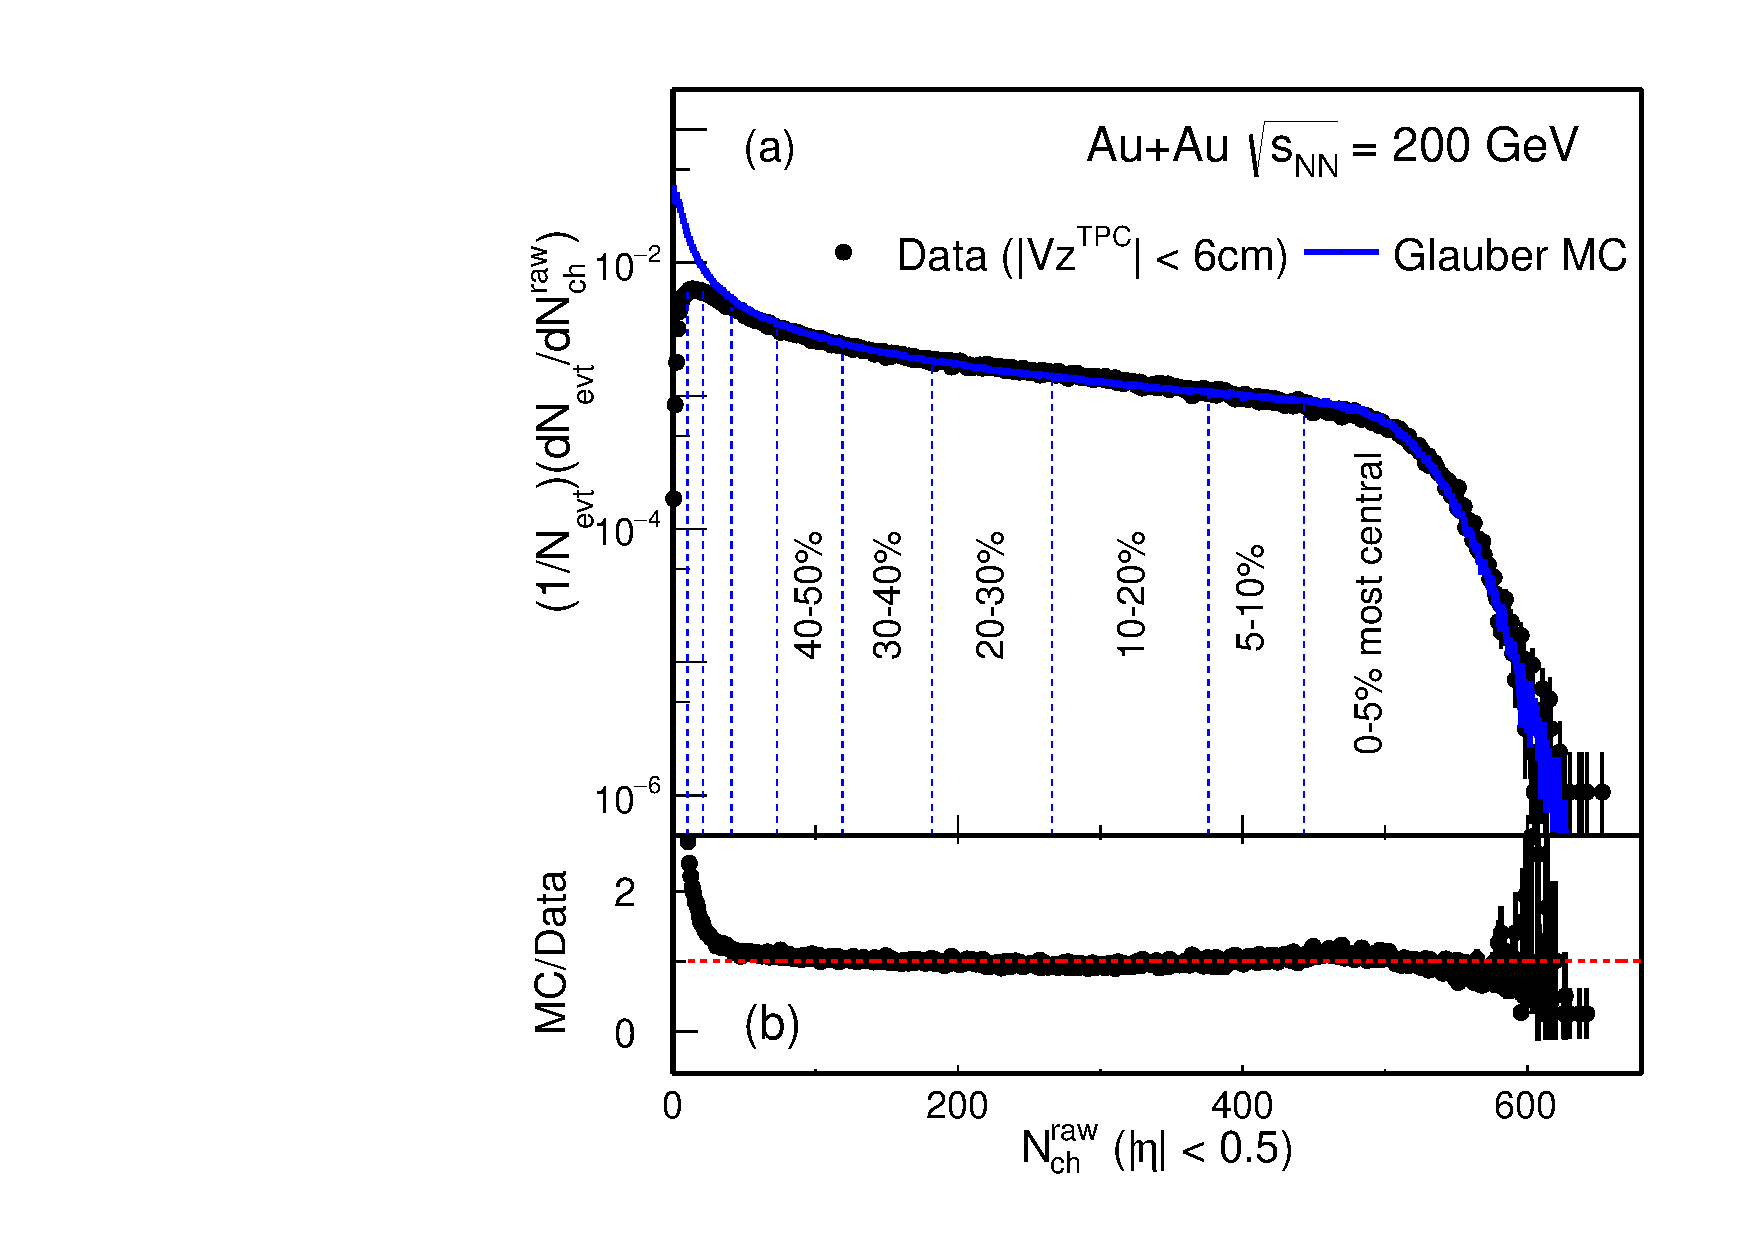
\includegraphics[width=0.45\textwidth]{fig/centrality.pdf}
\caption{(a) Uncorrected charged particle multiplicity $N_{\rm ch}^{\rm raw}$ distribution measured with $|\eta|$ $<$ 0.5 and $|Vz|$ $<$ 6 cm. The solid curve depicts the multiplicity distribution from a MC Glauber simulation fit to the experimental data. (b) Ratio between MC simulation and real data}
\label{fig:centrality} 
\end{figure}

\begin{figure*}
\centering
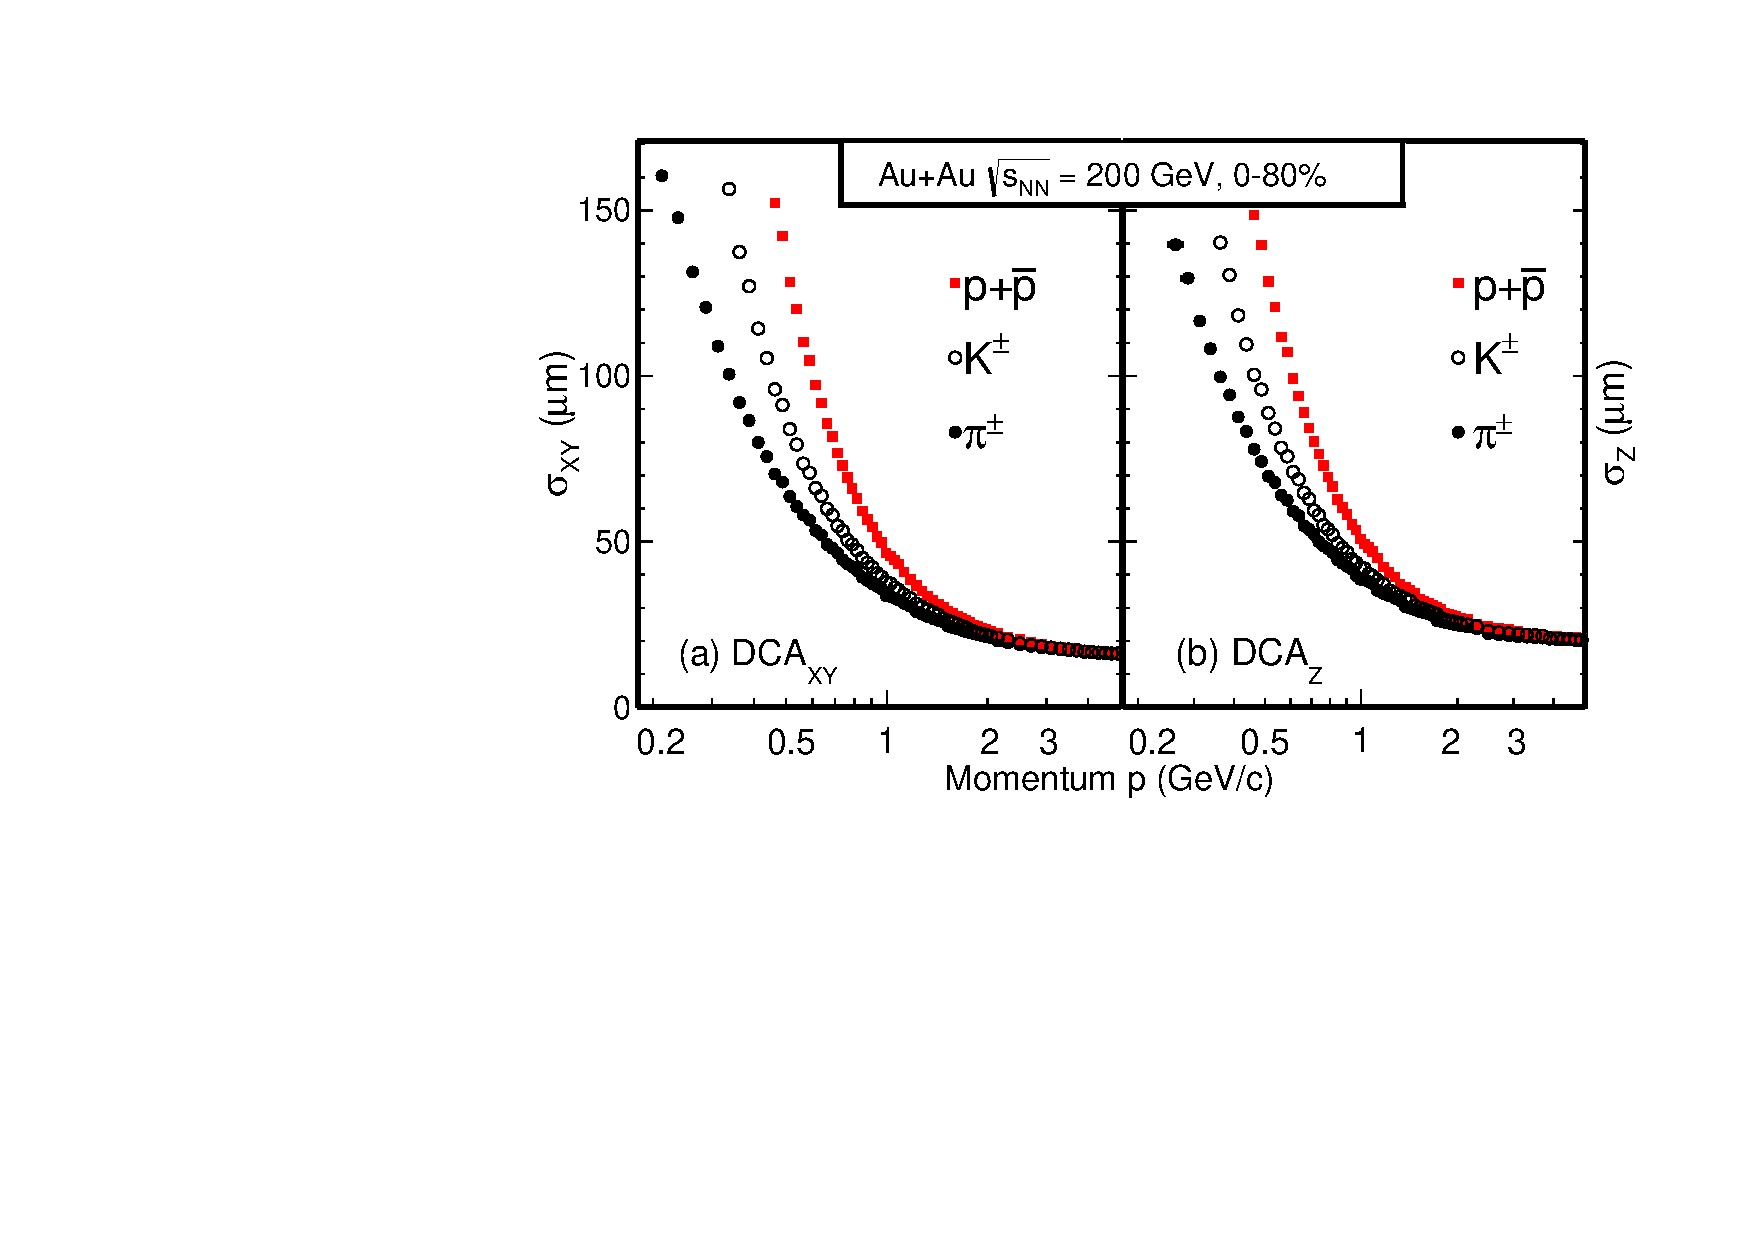
\includegraphics[width=0.85\textwidth]{fig/DCAXy_Z.pdf}
\caption{Identified particle ($\pi^{\pm}$, $K^{\pm}$, and $p$+$\bar{p}$) pointing resolution in the transverse (a) and longitudinal (b) planes as a function of particle total momentum in Au+Au 0--80\% collisions at $\sqrt{s_{_{\rm NN}}}$ = 200\,GeV.}
\label{fig:DCAXy_Z} 
\end{figure*}

\begin{figure}[h]
\centering
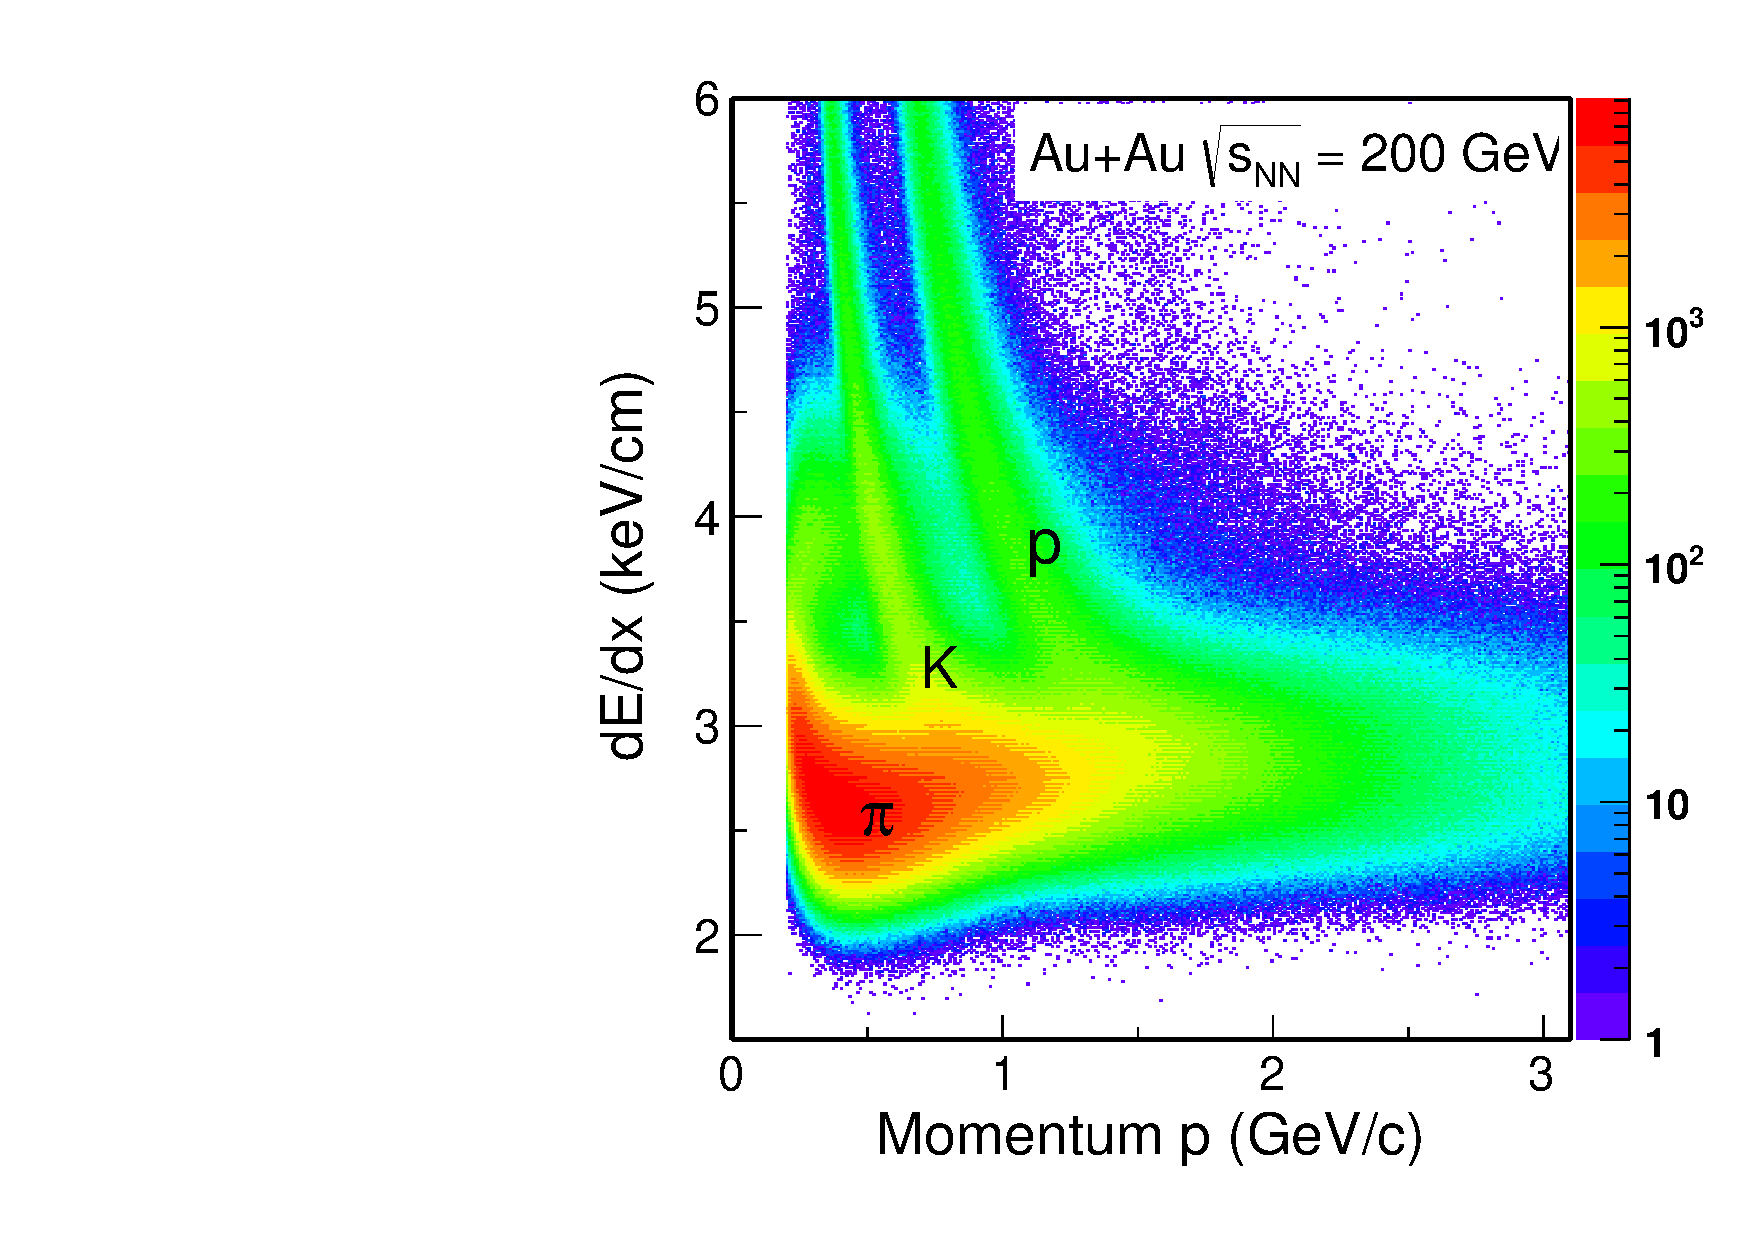
\includegraphics[width=0.45\textwidth]{fig/PID_dEdx.pdf}
\caption{TPC $dE/dx$ vs. particle momentum in Au + Au collisions at $\sqrt{s_{_{\rm NN}}}$ = 200\,GeV.}
\label{fig:PID_dEdx} 
\end{figure}

\begin{figure}[h]
\centering
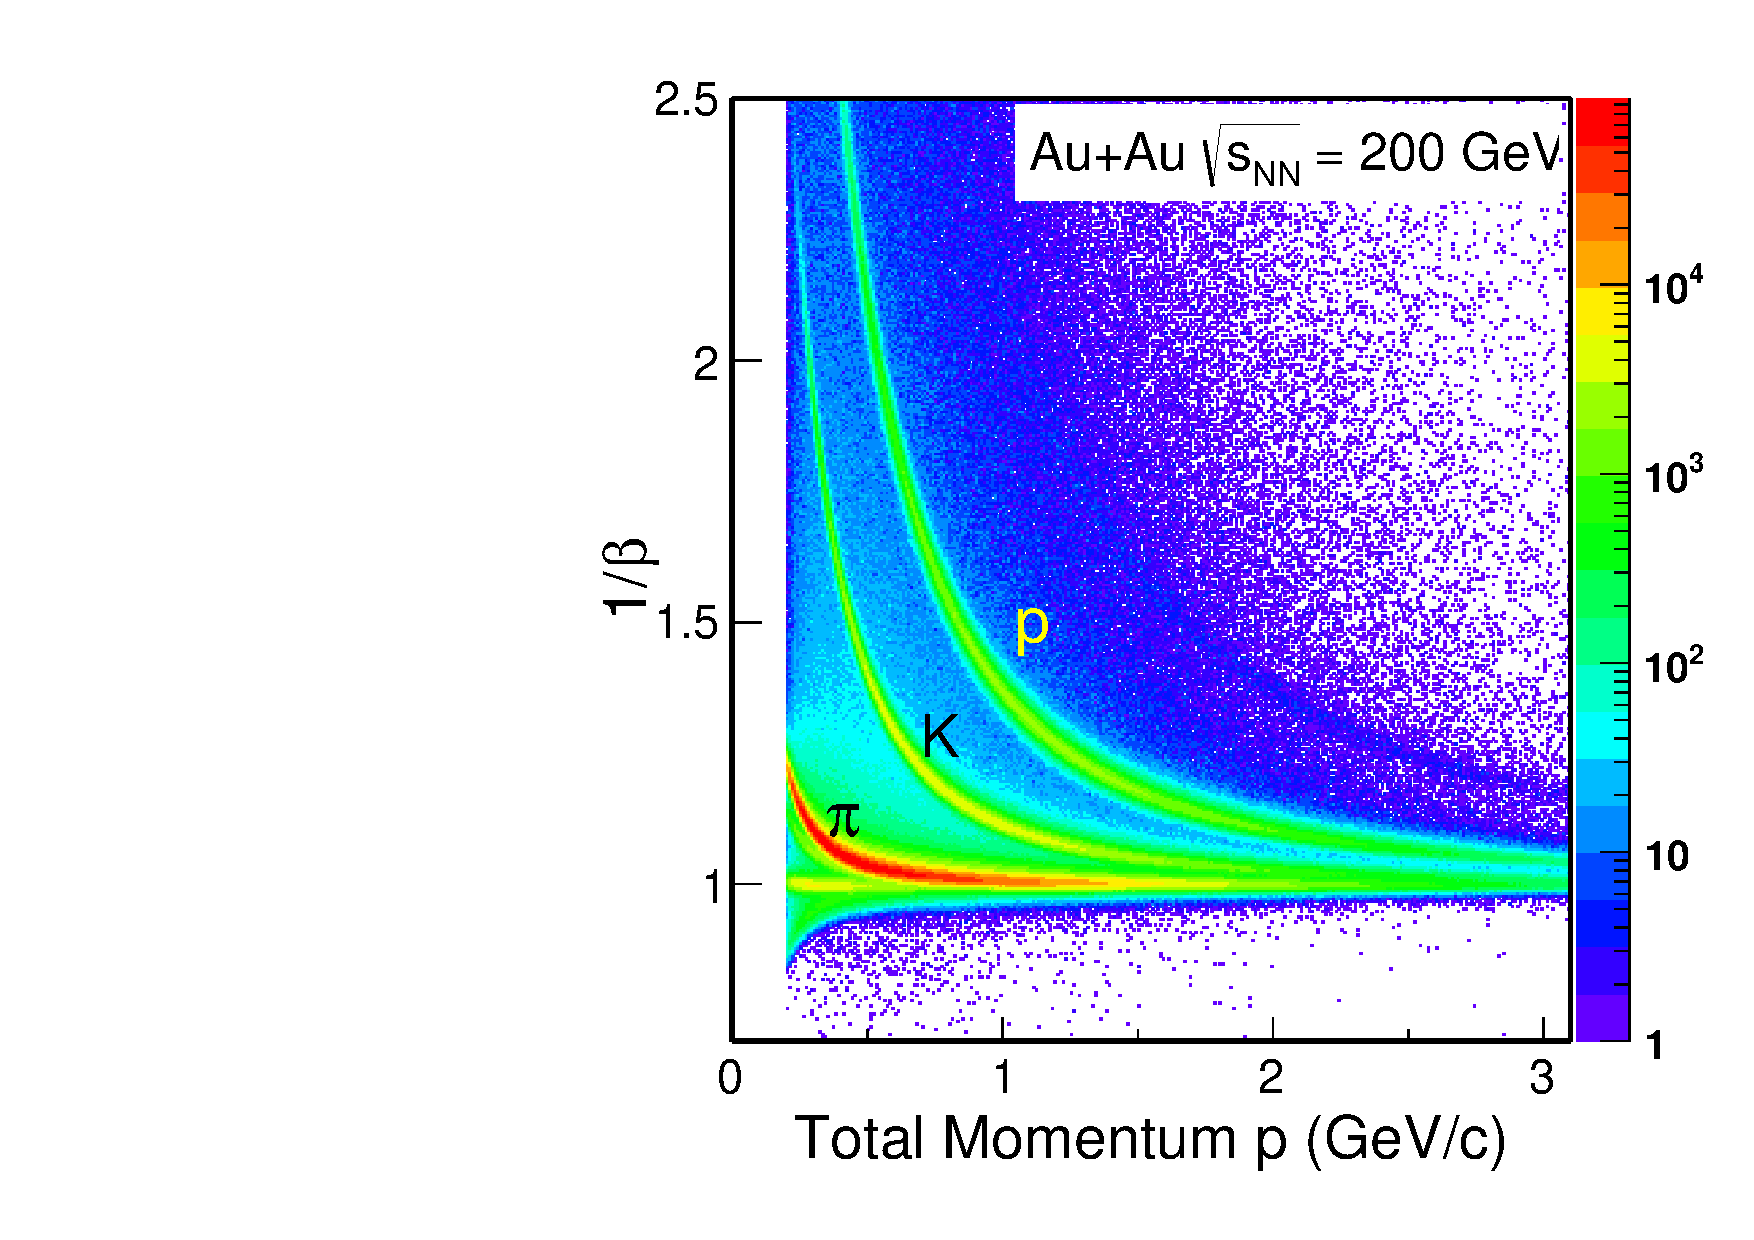
\includegraphics[width=0.45\textwidth]{fig/PID_beta.pdf}
\caption{TOF $1/\beta$ vs. particle momentum in Au + Au collisions at $\sqrt{s_{_{\rm NN}}}$ = 200\,GeV.}
\label{fig:PID_beta} 
\end{figure}

% Table~\ref{table:ccentrality} 
Table I lists the extracted values of number of binary collisions ($N_{\rm bin}$), number of participants ($N_{\rm part}$) and trigger inefficiency correction factors ($\varepsilon_{\rm trg}$) as well as their uncertainties. The $\varepsilon_{\rm trg}$ factors are average values over in each centrality bins, while in practice we apply this correction factor event-by-event according to the measured $N_{\rm ch}^{\rm raw}$ of the event.

\begin{table*}[t]
\centering{
  \caption{Estimated values of number of binary collisions ($N_{\rm bin}$), number of participants ($N_{\rm part}$) and trigger correction factors ($\varepsilon_{\rm trg}$, uncertainties negligible) for various centrality bins obtained from the MC Glauber model fit to the measured multiplicity distributions.}
\begin{tabular}{rcccccccc} \hline \hline
\hspace{1cm}Centrality\hspace{1cm} & \multicolumn{3}{c}{$N_{\rm bin}$} & \hspace{1cm} & \multicolumn{3}{c}{$N_{\rm part}$} & \hspace{1cm}$\varepsilon_{\rm trg}$\hspace{1cm} \\ \hline
0--10 \%\hspace{1cm}      & 938.8 & $\pm$ & 26.3 & & 319.4 & $\pm$ & 3.4  & 1.0 \\
10--20 \%\hspace{1cm}     & 579.9 & $\pm$ & 28.8 & & 227.6 & $\pm$ & 7.9  & 1.0 \\
20--40 \%\hspace{1cm}     & 288.3 & $\pm$ & 30.4 & & 137.6 & $\pm$ & 10.4 & 1.0 \\
40--60 \%\hspace{1cm}     & 91.3  & $\pm$ & 21.0 & & 60.5  & $\pm$ & 10.1 & 0.92 \\
60--80 \%\hspace{1cm}     & 21.3  & $\pm$ & 8.9  & & 20.4  & $\pm$ & 6.6  & 0.65 \\ \hline \hline
\end{tabular}
}
\label{table:ccentrality}
\end{table*}

\subsection{\label{sec:dataset:hft}Heavy Flavor Tracker}
The HFT~\cite{HFTQM14} is a high resolution silicon detector system, that aims for the topological reconstruction of secondary decay vertices. It consists of three silicon subsystems: the Silicon Strip Detector (SSD), the Intermediate Silicon Tracker (IST), and the two layers of PiXeL (PXL) detector. 
% Table~\ref{table:HFT} 
Table II lists the key characteristic parameters of each subsystem. The SSD detector is still in the commissioning stage when the dataset used in this analysis are taken, and therefore is not used in the offline data production and this analysis.
%They lay inside the TPC with incrementally improved resolution, SSD sit away from the beam with a radius $\sim$ 22 cm, IST around $\sim$ 14 cm and two layers of PXL with $\sim$ 8 cm and $\sim$ 2.8 cm respectively. 
The PXL detector uses the new Monolithic Active Pixel Sensors (MAPS) technology~\cite{PXL}. This is the first application of this technology in a collider experiment. It is particularly designed to measure heavy-flavor hadron decays in the high multiplicity heavy-ion collision environment.

%%% Need to confirm all the numbers
\begin{table*}[t]
\centering{
\caption{Several key characteristic parameters for each subsystem of the HFT detector.}
\begin{tabular}{ccccc} \hline \hline
\hspace{0.5cm}Subsystem\hspace{0.5cm} & \hspace{0.5cm}Radii (cm)\hspace{0.5cm} & \hspace{0.5cm}Length (cm)\hspace{0.5cm} & \hspace{0.5cm}Thickness at $\eta=0$ ($X_{0}$)\hspace{0.5cm} & \hspace{0.5cm}Pitch Size ($\mu m^2$)\hspace{0.5cm} \\ \hline
PXL inner layer & 2.8 & 20 & 0.52\% (0.39\%$^{\dagger}$) & 20.7$\times$20.7 \\
PXL outer layer & 8.0 & 20 & 0.52\% & 20.7$\times$20.7 \\
IST & 14.0 & 50 & 1.0\% & 600$\times$6000 \\
SSD$^{\dagger\dagger}$ & 22.0 & 106 & 1.0\% & 95$\times$40000 \\ \hline \hline
\end{tabular} \\
$^{\dagger}$ - PXL inner detector material is reduced to 0.39\%$X_0$ in 2015/2016 runs. \\
$^{\dagger\dagger}$ - SSD is not included in this analysis.}
\label{table:HFT} 
\end{table*}
% The HFT participated in the full 2014 Au + Au 200GeV runs in STAR.

In the offline reconstruction, tracks are reconstructed in the TPC first and then extended to the HFT detector to find the best fit to the measured high resolution spacial points. The tracking algorithm with Kalman filter that considers various detector material effects is used in the track extension. Considering the background hits level at the PXL due to pileup hadronic and electromagnetic collisions, tracks are required to have at least one hit in each layer of IST and PXL subdetectors. Fig.~\ref{fig:DCAXy_Z} shows the track pointing resolution to the primary vertex in the transverse plane ($\sigma_{\rm XY}$) in panel (a) and along the longitudinal direction ($\sigma_{\rm Z}$) in panel (b) as a function of momentum ($p$) for identified particles in 0-80\% centrality Au + Au collisions at $\sqrt{s_{\rm NN}}$ = 200\,GeV. The design goal for the HFT detector is to have a pointing resolution better than 55 $\mu m$ for 750\,MeV Kaons. Fig.~\ref{fig:DCAXy_Z} demonstrates that the HFT detector system has delivered a performance that satisfies the requirements for open heavy flavor physics measurements.


% Chapter three
\section{\label{sec:D0recon}$D^0$-meson reconstruction}

$D^0$ and $\overline{D}^{0}$ mesons are reconstructed via the hadronic decay channel $D^0\rightarrow K^-+\pi^+$ and its charge conjugate channel with a branching ratio of 3.89\%. In what follows, we imply $(D^0 +\overline{D}^{0})/2$ when using the term $D^0$ unless otherwise specified. $D^0$ mesons decay with a proper decay length of $c\tau\sim123\ \mu$m after they are produced in Au+Au collisions. We utilize the high pointing resolution capability enabled by the HFT detector to topologically reconstruct the $D^0$ decay vertices that are separated from the collision vertices, which drastically reduces the combinational background and improves the measurement precision.

Charged pion and kaon tracks are reconstructed with the TPC and the HFT. Tracks are required to have at least 20 measured TPC points out of maximum 45 to ensure good momentum measurement. To enable high pointing precision, both daughter tracks are required to have at least one measured hit in each layer of PXL and IST as described above. Particle identification is achieved via a combination of the ionization energy loss ($dE/dx$) measurement in the TPC and the $tof$ measurement in the TOF. The resolution-normalized $dE/dx$ deviation from the expected values is defined as:
\[
% N\sigma_X = \frac{dE/dx_{mea}-dE/dx_{th}}{R}
n\sigma_X = \frac{1}{R}\ln\frac{\langle{dE/dx}\rangle_{mea.}}{\langle{dE/dx}\rangle_{X}}
\]
Where $\langle{dE/dx}\rangle_{mea.}$ and $\langle{dE/dx}\rangle_{X}$ represent measured and theoretical $dE/dx$, and $R$ is the STAR TPC $dE/dx$ resolution (typically $\sim$8\%). The $n\sigma_X$ should be close to a standard Gaussian distribution for each corresponding particle species (mean $=$ 0, $\sigma = $ 1).
Pion (kaon) candidates are selected by a requirement of the measured $dE/dx$ to be within three (two) standard deviation ($|n\sigma_{X}|$) from the expected values. When tracks have matched hits in the TOF detector, an additional requirement on the measured particle velocity ($\beta$) to be within three standard deviation from the expected values ($|\Delta 1/\beta|$) is applied for either daughter track. Fig.~\ref{fig:PID_dEdx} and Fig.~\ref{fig:PID_beta} show an example of the particle identification capability from TPC and TOF. Tracks within the kinematic acceptance $p_{\rm T}>0.6$ GeV/$c$ and $|\eta|<1$) are used to combine and make pairs. Table~\ref{table:singlecut} lists the TPC and TOF selection cuts for daughter kaon and pion tracks used for $D^0$ reconstruction.

\begin{table}
\centering{
\caption{TPC and TOF selection cuts for $K$ and $\pi$ tracks.}
\begin{tabular}{cccc} \hline \hline
Variable & & $K^{\mp}$  & $\pi^{\pm}$ \\ \hline
$p_{\rm T}$ (GeV/$c$)   & $>$ & 0.6 & 0.6 \\
$|\eta|$			    & $<$ & 1.0 & 1.0 \\
nHitsFit (TPC)		    & $>$ & 20  & 20 \\
% nHitsFit/nHitsMax (TPC) & $>$ & 0.52 & 0.52 \\
$|n\sigma_{X}|$         & $<$ & 2.0 & 3.0 \\
$|\Delta 1/\beta|$ (if $\beta>0$)     & $<$ & 0.03 & 0.03 \\ \hline \hline
\end{tabular}
}
\label{table:singlecut} 
\end{table}

\begin{figure*}
\centering
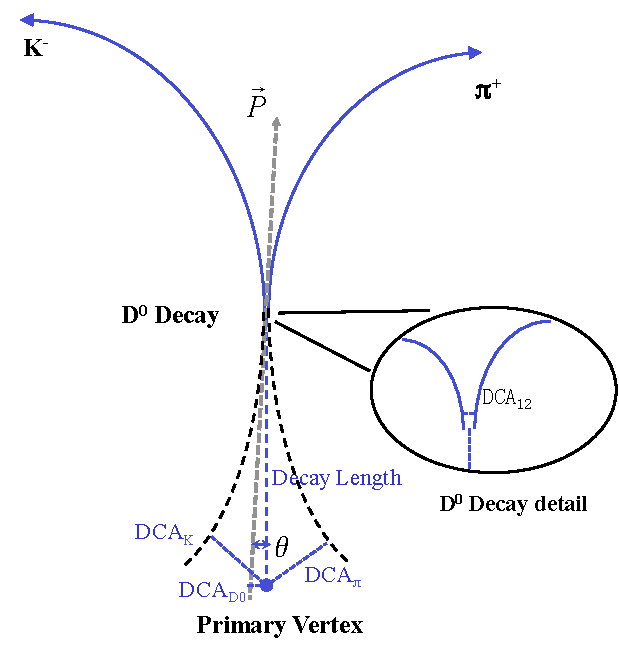
\includegraphics[width=0.6\textwidth]{fig/D0carton.pdf}
\caption{$D^{0}$ topological variables used in the reconstruction.}
\label{fig:D0carton} 
\end{figure*}

With a pair of two daughter tracks, pion and kaon, the $D^0$ decay vertex is reconstructed as the middle point on the distance of the closet approach between the two daughter trajectories. The background is mainly due to the random combination of the fake pairs directly from the collision point. With the following topological variables, the background can be greatly reduced.

\begin{itemize}
  \item Decay Length: the distance between the reconstructed decay vertex and the primary vertex (PV).
  \item Distance of Closest Approach (DCA) between the 2 daughter tracks. ($\rm DCA_{12}$)
  \item DCA between reconstructed $D^0$ and the PV. ($\rm DCA_{D^{0}}$)
  \item DCA between the pion and the PV. ($\rm DCA_{\pi}$)
  \item DCA between the kaon and the PV. ($\rm DCA_{K}$)
  \item Angle between $D^0$ momentum and the line between the reconstructed decay vertex and the PV. ($\theta$)
\end{itemize}

The carton Fig.~\ref{fig:D0carton} also shows the topological variables used in the analysis, where $\vec{P}$ represent the $D^0$ momentum. The Decay Length and cos($\theta$) follow the formula : $\rm DCA_{D^{0}}$ = Decay Length $\times$ sin($\theta$). The cuts on the topological variables for this analysis are optimized using a Toolkit for Multivariate Data Analysis (TMVA) package in order to have the greatest signal significance. We explored several different discrimination methods in the TMVA package and the Rectangular cut optimisation method is chosen for best signal significance estimation. The optimization is conducted for different $D^0$ $p_{\rm T}$ bins and difference centrality bins. Table~\ref{table:topocut} lists a typical set of topological cuts for 0-10\% central Au+Au collisions.

\begin{table*}[t]
\centering {
\caption{$D^0$ topological cuts for the 0-10\% most central collisions in separated $p_T$ ranges.}
\begin{tabular}{cc|ccccccc} \hline \hline
$0-10\% \ |\ p_{\rm T}$ (GeV/$c$) &    & \hspace{0.5cm}(0,0.5)\hspace{0.5cm} & \hspace{0.5cm}(0.5,1)\hspace{0.5cm} & \hspace{0.5cm}(1,2)\hspace{0.5cm} & \hspace{0.5cm}(2,3)\hspace{0.5cm} & \hspace{0.5cm}(3,5)\hspace{0.5cm} &  \hspace{0.5cm}(5,8)\hspace{0.5cm} &  \hspace{0.5cm}(8,10)\hspace{0.5cm} \\ \hline
  Decay Length ($\mu m$) & $>$ & 100 & 199 & 227 & 232 & 236 & 255 & 255 \\
  $\rm DCA_{12}$        ($\mu m$) & $<$ & 71  & 64 & 70 & 63 & 82 & 80 & 80 \\
  $\rm DCA_{D^{0}}$       ($\mu m$) & $<$ & 62  & 55 & 40 & 40 & 40 & 44 & 44 \\
  $\rm DCA_{\pi}$  ($\mu m$) & $>$ & 133 & 105 & 93 & 97 & 67 & 55 & 55 \\
  $\rm DCA_{K}$    ($\mu m$) & $>$ & 138 & 109 & 82 & 94 & 76 & 54 & 54 \\ 
  $\cos(\theta)$          & $>$ & 0.95 & 0.95 & 0.95 & 0.95 & 0.95 & 0.95 & 0.95 \\ \hline \hline
\end{tabular}
\label{table:topocut}
}
\end{table*}

\begin{figure*}
\centering
% 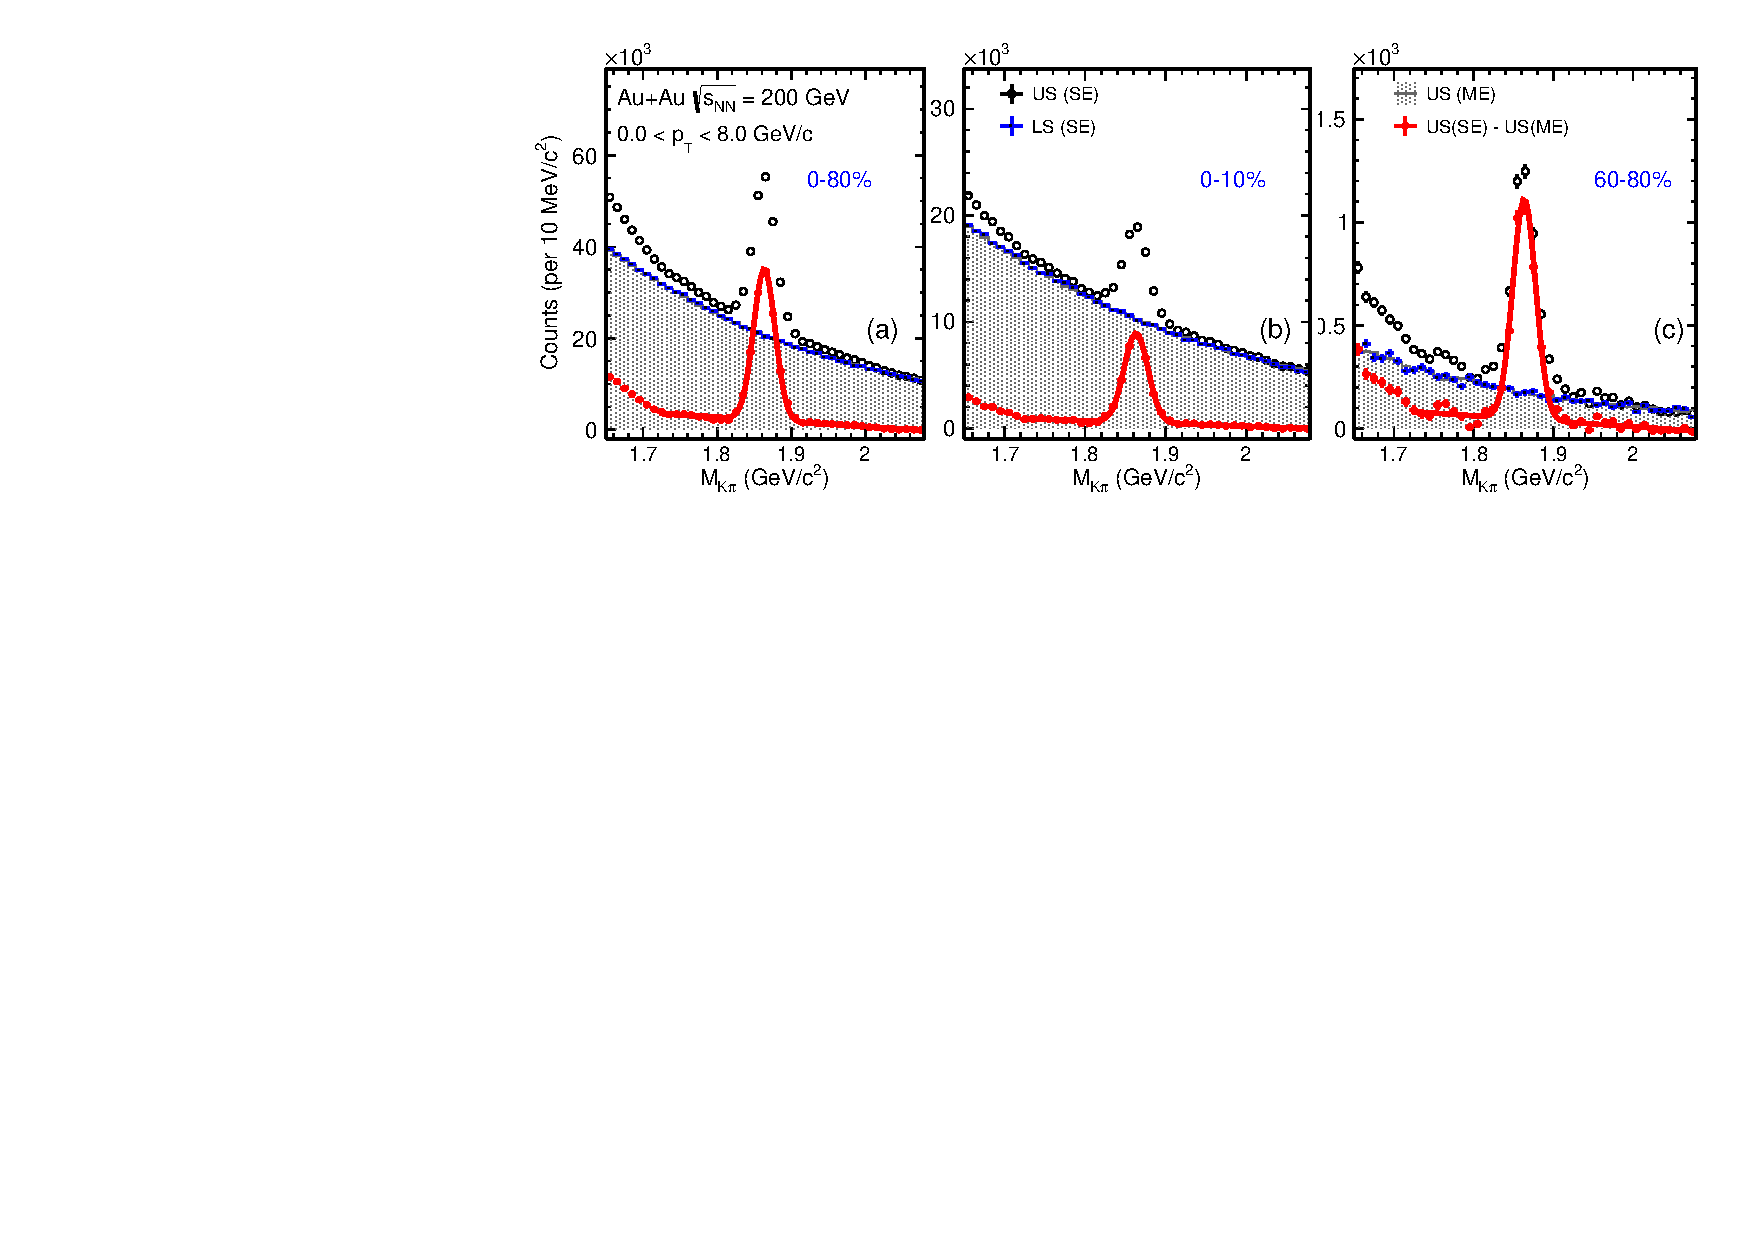
\includegraphics[width=1.0\textwidth]{fig/signal_0_8GeV.pdf}
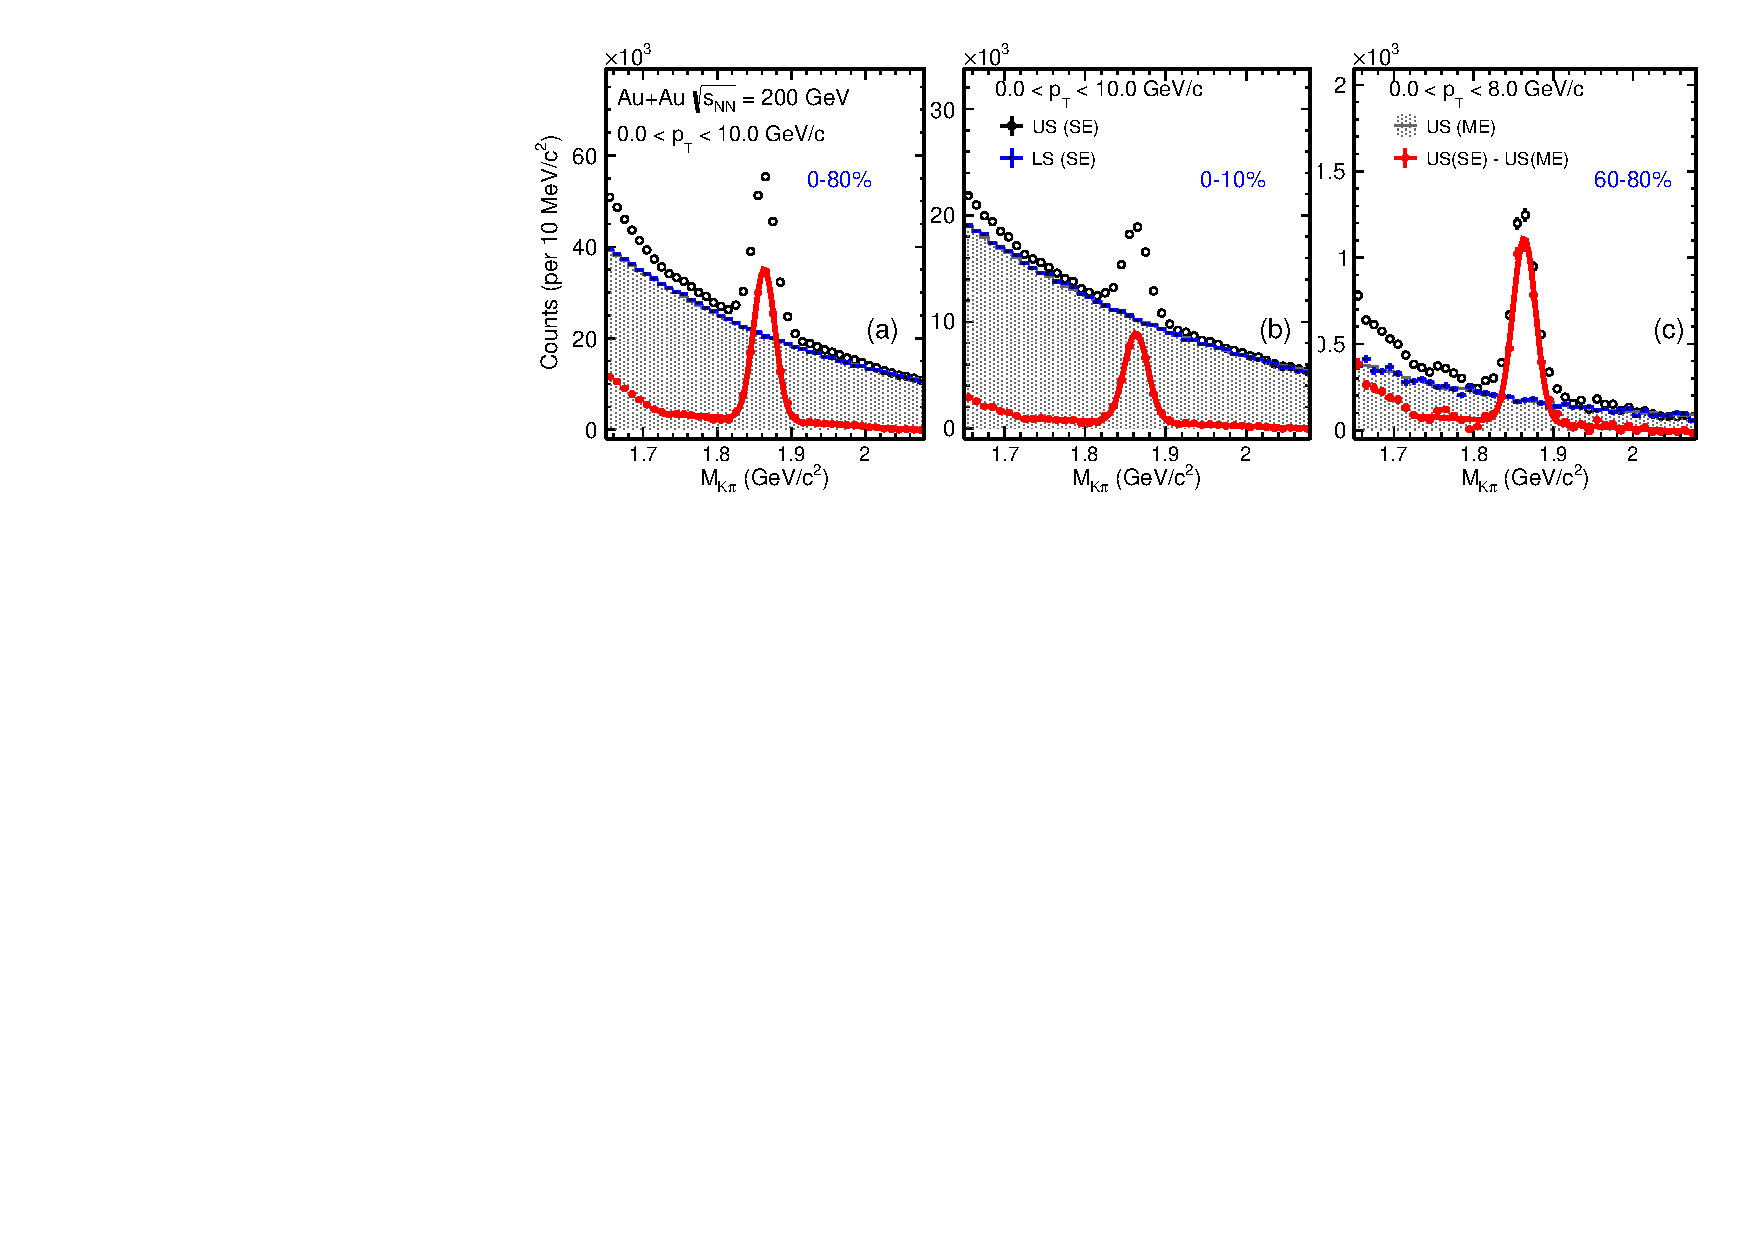
\includegraphics[width=1.0\textwidth]{fig/signal_0_8_10GeV.pdf}
\caption{Invariant mass $\rm M_{K\pi}$ distributions in $0 < p_{\rm T} < 10$ GeV/c from centrality bins 0--80\% (a), 0--10\% (b) and $0 < p_{\rm T} < 8$ GeV/c for 60--80\% (c), respectively in Au+Au collisions at $\sqrt{s_{_{\rm NN}}}$ = 200\,GeV. The upper limit $p_T$ range for 60--80\% stopped at 8 GeV/c since there is no signal beyond.}
\label{fig:signal_0} 
\end{figure*}

\begin{figure*}
\centering
% 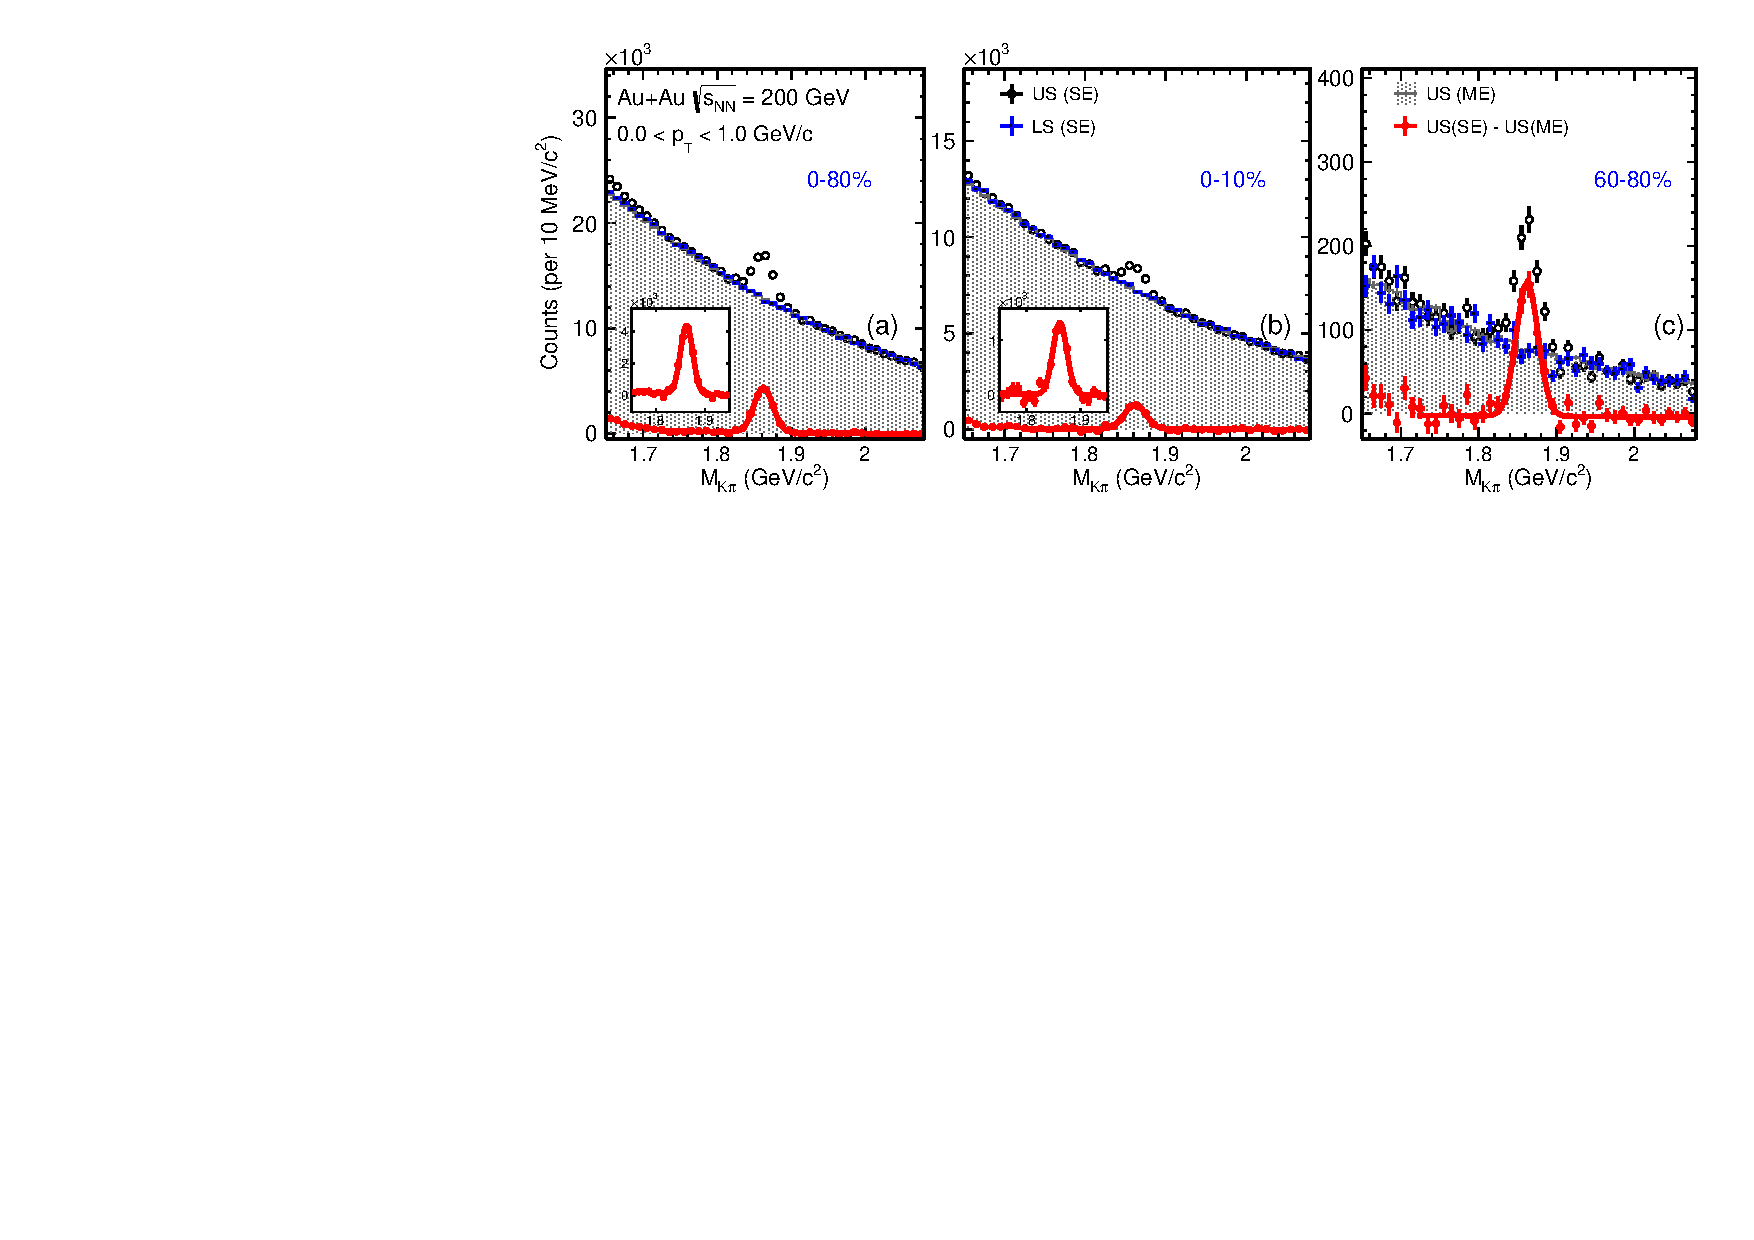
\includegraphics[width=1.0\textwidth]{fig/signal2_0_1GeV.pdf}
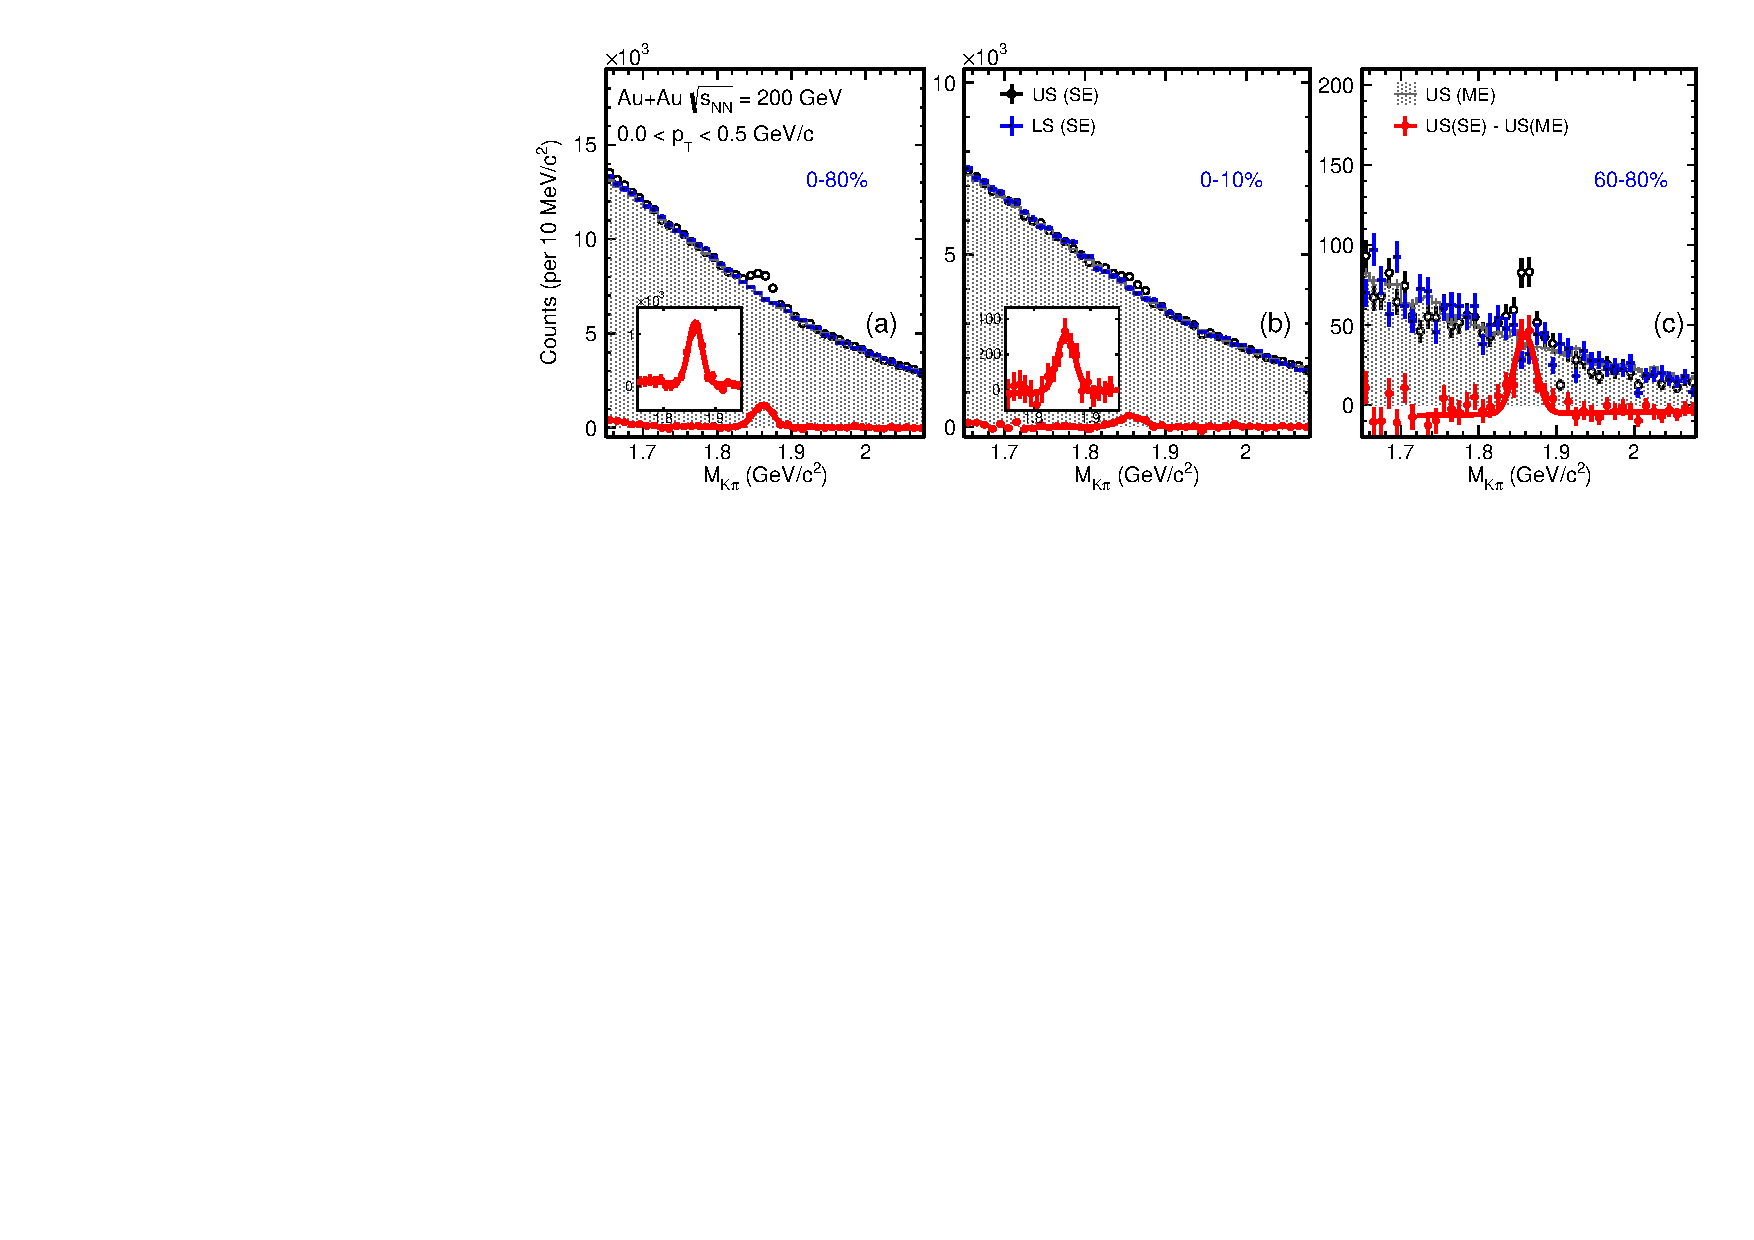
\includegraphics[width=1.0\textwidth]{fig/signal2_0_05GeV.pdf}
\caption{Invariant mass $\rm M_{K\pi}$ distributions in $0 < p_{\rm T} < 0.5$ GeV/c from centrality bins 0--80\% (a), 0--10\% (b) and 60--80\% (c), respectively in Au+Au collisions at $\sqrt{s_{_{\rm NN}}}$ = 200\,GeV.}
\label{fig:signal_1} 
\end{figure*}

\begin{figure*}
\centering
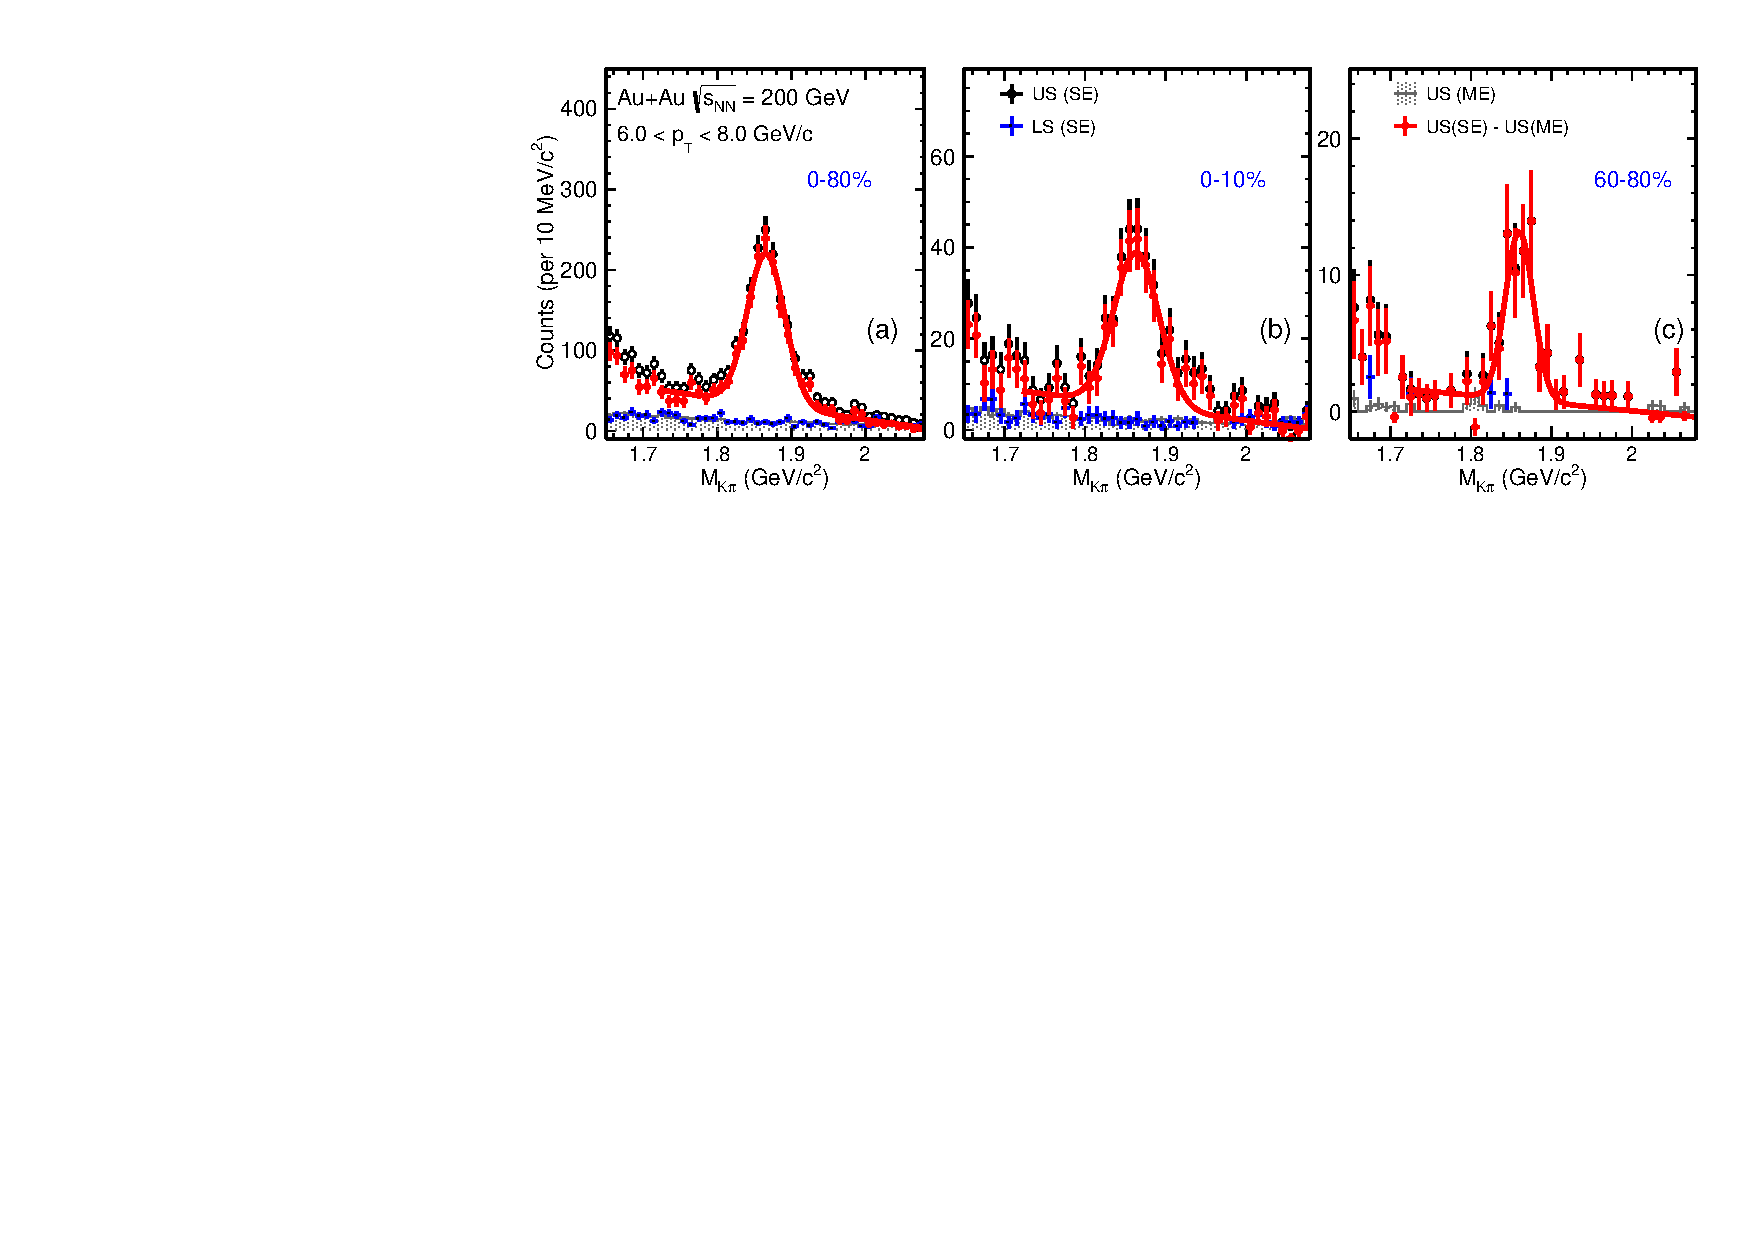
\includegraphics[width=1.0\textwidth]{fig/signal_6_8GeV.pdf}
\caption{Invariant mass $\rm M_{K\pi}$ distributions in $6 < p_{\rm T} < 8$ GeV/c from centrality bins 0--80\% (a), 0--10\% (b) and 60--80\% (c), respectively in Au+Au collisions at $\sqrt{s_{_{\rm NN}}}$ = 200\,GeV.}
\label{fig:signal_2} 
\end{figure*}

Figure~\ref{fig:signal_0} shows the invariant mass spectra of $K\pi$ pairs in 0-8 GeV/$c$ for three different centralities, 0-80\% minimum bias events, 0-10\% most central collisions and 40-80\% peripheral collisions, respectively. The combinatorial background is estimated with the same event like-sign pairs (grey) and the mixed event unlike-sign (blue) technique in which $K$ and $\pi$ from different events of similar characteristics ($V_{Z}$, centrality, event plane angle) are paired. The mixed event spectra are normalized to the like-sign distributions in the mass range from 1.7 to 2.1 GeV/$c^2$. After the subtraction of the mixed event combinatorial background from the unlike sign pairs (grey circle), the rest are shown as red circles in the plot. Compared to the previous $D^0$ study ~\cite{Star_D_RAA}, the $D^0$ signal significance is largely improved due to the combinatorial background rejection using the topological cuts enabled by the installation of HFT. 

Figure~\ref{fig:signal_1} and Fig.~\ref{fig:signal_2} shows the invariant mass spectra at the same centralities as Fig.~\ref{fig:signal_0} but for different $p_T$ ranges, one is for the lowest range 0 $< p_T <$ 1 GeV/c and another one for the highest range 6 $< p_T <$ 8 GeV/c.

After the combinatorial background is subtracted, the residual $K\pi$ invariant mass distributions are then fit by a Gaussian plus linear polynomial function. %The $D^0$ raw yields are calculated using the histogram counting within the $D^0$ mass peak region subtracting the residual background estimated via either a side-band method or a polynomial function fit.
The $D^0$ raw yields are extracted from the fits while the residual background are estimated via a polynomial function fit.

\section{\label{sec:correction}Efficiencies and Corrections}
The reconstructed $D^0$ raw yields are calculated in each centrality, $p_{\rm T}$ bin and within the rapidity window $|y|<1$. The fully corrected $D^0$ production invariant yields are calculated using the following formula.

%\lipsum[1]
\begin{widetext}
\[
  \frac{d^2N}{2\pi p_{\rm T}dp_{\rm T}dy} = \frac{1}{\rm B.R.} \frac{N^{\rm raw}}{N_{\rm evt} 2\pi p_{\rm T}\Delta p_{\rm T}\Delta y} \frac{1}{\varepsilon_{\rm trg}\times\varepsilon_{\rm TPC}\times\varepsilon_{\rm HFT}\times\varepsilon_{\rm PID}\times\varepsilon_{\rm vtx}}
\]
\label{equ:invariantyield}
\end{widetext}
%\lipsum[1]

where B.R. is the $D^0\rightarrow K^-\pi^+$ decay branching ratio, (3.89$\pm$0.04)\%. $N^{\rm raw}$ is the reconstructed $D^0$ raw counts. $N_{\rm evt}$ is the total numbers of events used for this analysis. $\varepsilon_{\rm trg}$ is the centrality bias correction factor described in Sec.~\ref{sec:dataset:trigger}. The raw yields need to be corrected for the TPC acceptance and tracking efficiency - $\varepsilon_{\rm TPC}$, the HFT acceptance and tracking plus topological cut efficiency - $\varepsilon_{\rm HFT}$, the particle identification efficiency - $\varepsilon_{\rm PID}$ and the finite vertex resolution correction - $\varepsilon_{\rm vtx}$, mostly in small multiplicity peripheral events. These four corrections will be discussed in detail in the following part of this sub-section.

\subsection{\label{sec:correction:tpc}TPC Acceptance and Tracking Efficiency - $\varepsilon_{\rm TPC}$}

The TPC acceptance and tracking efficiency is obtained using the standard STAR TPC embedding technique, in which a small amount of MC tracks (typically 5\% of the total multiplicity of the real event) are processed through the full GEANT simulation, then mixed with the raw Data Acquisition (DAQ) data in real events and reconstructed through the same reconstruction chain as the real data production. The TPC efficiency is then calculated as the ratio of the reconstructed MC tracks with the same offline analysis cuts for geometric acceptance and other TPC requirements to the input MC tracks.

Figure~\ref{fig:Datad0Eff_tpc} shows the TPC acceptance and tracking efficiencies $\varepsilon_{\rm TPC}$ for $D^0$ mesons in various centrality classes in Au+Au collisions at $\sqrt{s_{_{\rm NN}}}$ = 200\,GeV in this analysis. The efficiencies include the TPC and analysis acceptance cuts $p_{\rm T}>0.6$\,GeV/$c$ and $|\eta|<1$ as well as the TPC tracking efficiency for both pion and kaon daughters. The lower efficiency observed in central collisions is due to the increased multiplicity, and therefore higher occupancy, in these collisions.

\begin{figure}
\centering
% 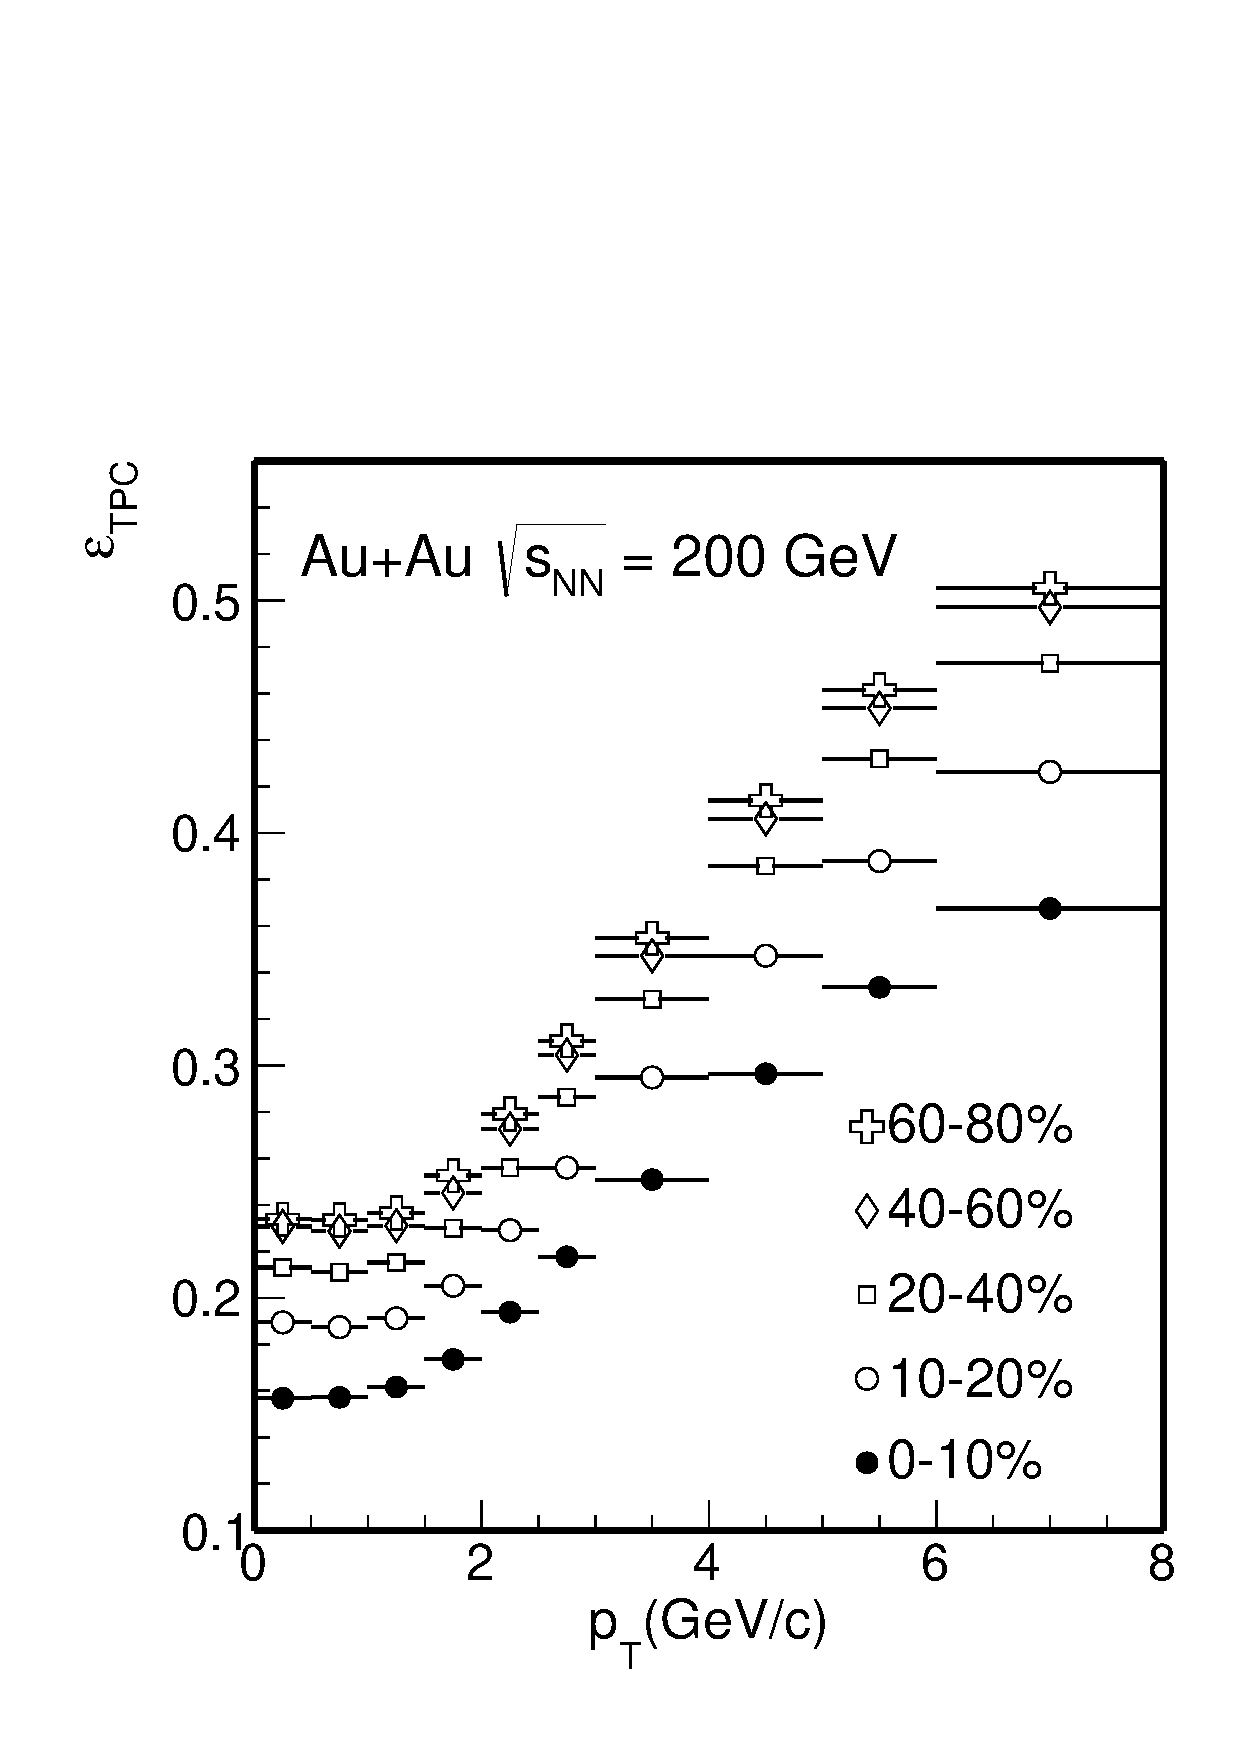
\includegraphics[width=0.4\textwidth]{fig/Datad0Eff_tpc.pdf}
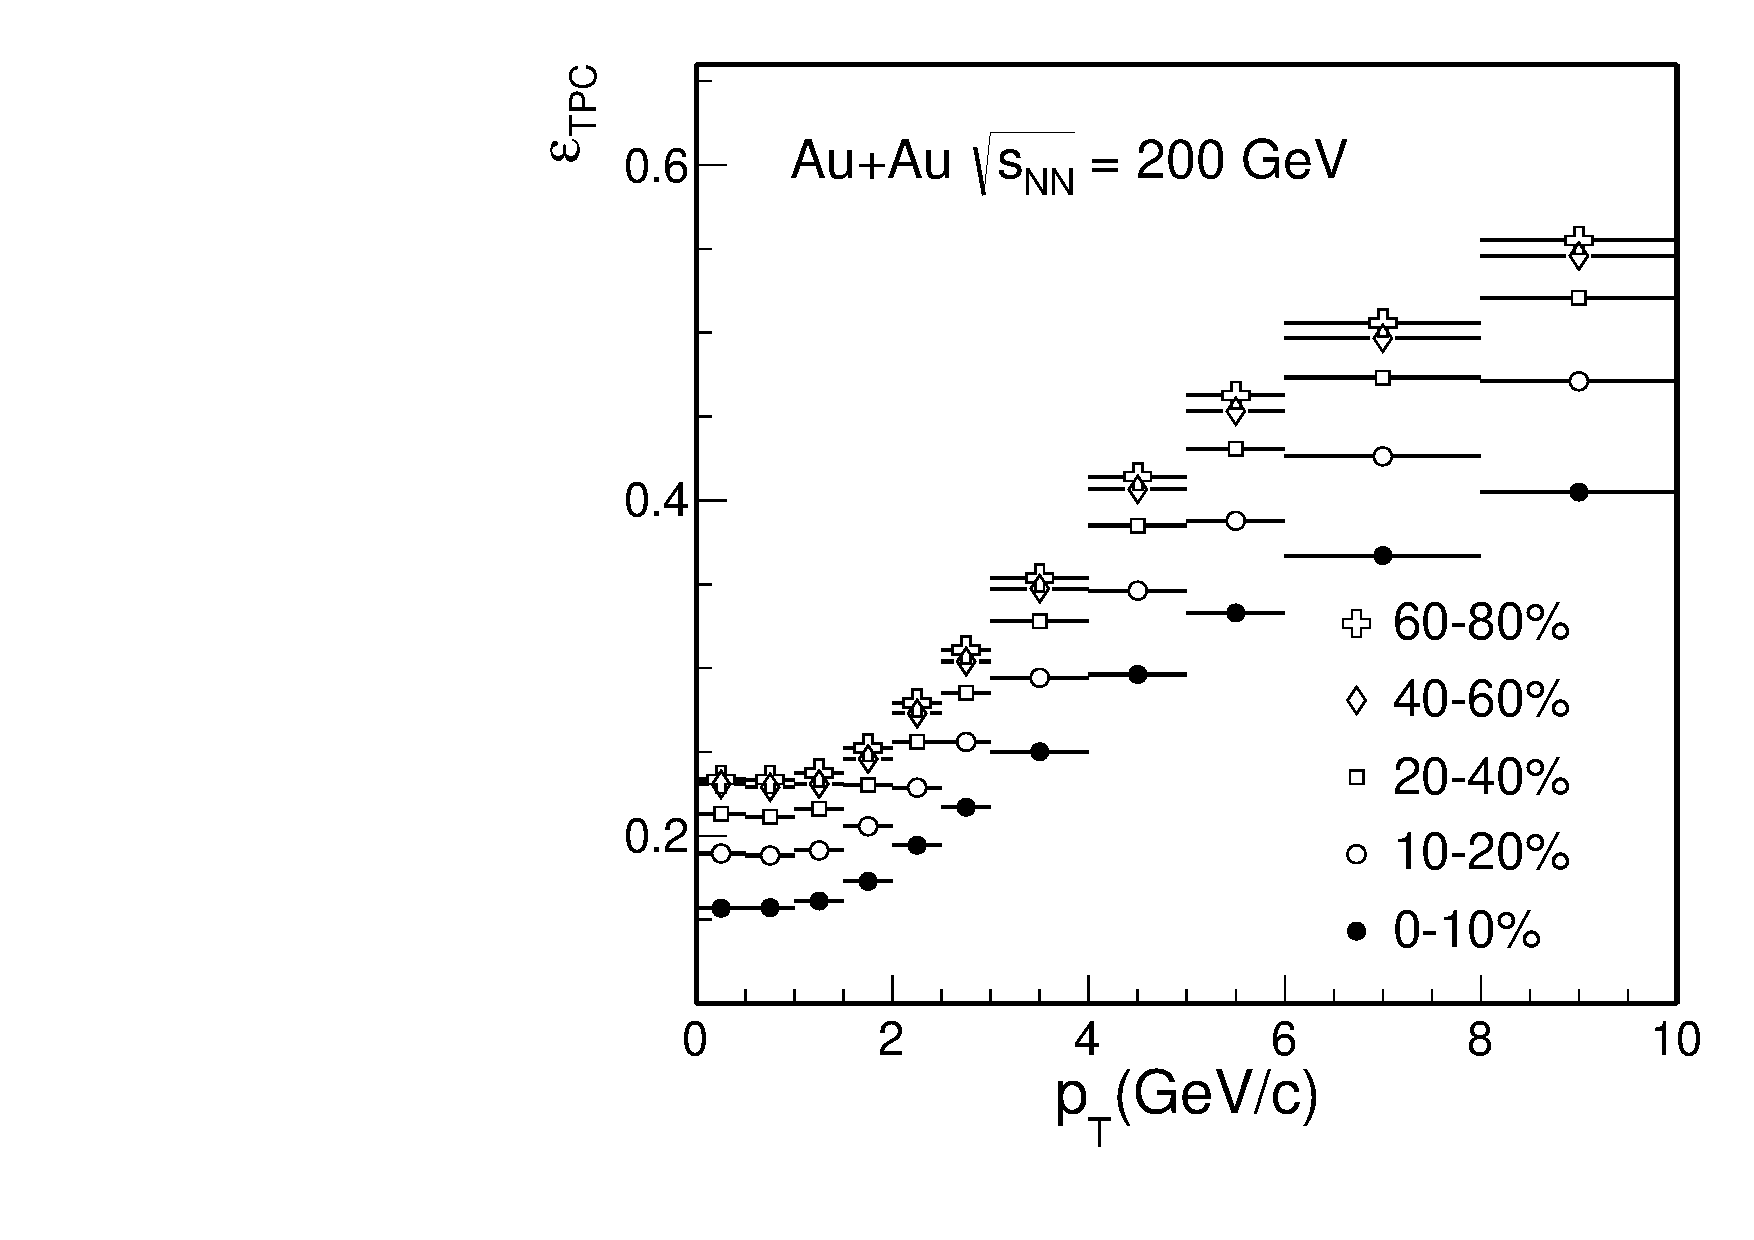
\includegraphics[width=0.43\textwidth]{fig/Datad0Eff_tpc_10.pdf}
\caption{$D^{0}$ TPC acceptance and tracking efficiencies from different centrality classes in Au + Au collisions at $\sqrt{s_{_{\rm NN}}}$ = 200\,GeV.}
\label{fig:Datad0Eff_tpc} 
\end{figure}


\subsection{\label{sec:correction:hft}HFT Acceptance, Tracking and Topological Cut Efficiency - $\varepsilon_{\rm HFT}$}

\subsubsection{\label{sec:correction:hft:fastsim}Data-driven Simulation}

Since the performance of the HFT changes with time, in order to fully capture the real-time detector performance the HFT-related efficiency is obtained using a data-driven simulation method in this analysis. The performance of inclusive HFT tracks is characterized by a TPC-to-HFT matching ratio and the DCA distributions. These distributions obtained from real data are fed into a Monte Carlo decay generator for $D^0\rightarrow K^-\pi^+$ and followed by the same reconstruction of $D^0$ secondary vertex as in real data. The same topological cuts are then be applied and the HFT related efficiency for the $D^0$ reconstruction is then calculated.

% To obtain the real invariant mass spectrum of $D^0$ within STAR acceptance ($|\eta_{\pi}| \leq 1, |\eta_{K}| \leq 1, |Y_{K\pi}| \leq 1$), the $D^0$ raw spectrum should correct for the efficiency. The $K\pi$ pair efficiency within STAR acceptance is evaluated by folding the TPC related efficiency to the HFT related efficiency as shown on Eq.~\ref{effEqu1} and Eq.~\ref{effEqu2}. For the TPC related tracking efficiency shows on the first term, we use STAR standard Full GEANT simulation. For the HFT related efficiency include the second and third terms which reflect to HFT acceptance and topological cuts, the developed `Data-Driven Fast simulation' which will discuss following.

% \begin{equation}
%   % \textup{Eff.} \times \textup{Accept.}  = \textup{TPC Tracking Eff.} \otimes \textup{HFT Tracking Eff.} \otimes \textup{Topollogy Cuts}
%   \textup{Eff.} \times \textup{Accept.}  = \textup{TPC Tracking Eff.} \otimes \textup{HFT Related Eff.}
% \label{effEqu1}
% \end{equation}

% \begin{equation}
%   \textup{HFT Related Eff.}  =\textup{HFT Tracking Eff.} \otimes \textup{Topology Cuts}
% \label{effEqu2}
% \end{equation}

To best represent the detector real performance, we obtain the following distributions from real data in this Monte Carlo approach.
\begin{itemize}
\item Centrality-dependent $\textup{V}_\textup{z}$ distributions.
\item Ratios of HFT matched tracks to TPC tracks, including the dependence on particle species, centrality, $p_T$, $\eta$, $\phi$, and $\textup{V}_\textup{z}$.
\item $\textup{DCA}_{\textup{XY}}$ - $\textup{DCA}_{\textup{Z}}$ 2-dimension (2D) distributions including the dependence on particle species, centrality, $p_T$, $\eta$, and $\textup{V}_\textup{z}$.
\end{itemize}
The $\textup{DCA}_{\textup{XY}}$ - $\textup{DCA}_{\textup{Z}}$ 2D distributions are the key to represent not only the right matches, but also the fake matches when connecting the TPC tracks with HFT hits. The distributions are obtained in 2D to consider the correlation between the two quantities and therefore to reproduce the 3D DCA position distributions. The $\phi$ dependence of these distributions are integrated over due to computing resource limits, but we have checked the $\phi$ dependence (by reducing other dependences for the same reason) and it produces a consistent efficiency result compared to the $\phi$-degenerated result we use here as the default.

In total, there are 11 ($\phi$) $\times$ 10 ($\eta$) $\times$ 6 ($\textup{V}_\textup{z}$) $\times$ 9 (centrality) $\times$ 2 (particles) 1D histograms (36 $p_T$ bins each) used for the HFT match ratio distributions and 5 ($\eta$) $\times$ 4 ($\textup{V}_\textup{z}$) $\times$ 9 (centrality) $\times$ 2 (particles) $\times$ 19 ($p_T$) 2D histograms (144 $\times$ 144 DCA binning) for 2D DCA distributions. The number of bins chosen is optimized to balance the need of computing resources as well as the stability of the final efficiency. All dimensions have been checked so that further increase in the number of bins (in balance we need to reduce the number of bins in other dimensions)  will not change the final obtained efficiency.

The procedure for this data-driven simulation package for efficiency calculation is as follows:

% After all the input ingredients ready for the fast-simulation, a simple toy MC simulation (PYTHIA) is applied for the efficiency study. The basic recipe is following:
\begin{itemize}
\item Sample $\textup{V}_\textup{z}$ distribution according to data distribution.
\item Generate $D^0$ at the event vertex position with desired $p_T$ (levy shape fitted to $D^0$ spectra) and rapidity (flat) distributions.
\item Let $D^0$ fly and decay to $K^-\pi^+$ daughters following the decay probability.
\item Smear daughter track momentum according to the values obtained from embedding.
\item Smear daughter track starting position according to the $\textup{DCA}_{\textup{XY}}$-$\textup{DCA}_\textup{Z}$ 2D distributions from the reconstructed data.
\item Apply HFT matching efficiency according to the HFT matching ratio distribution from the reconstructed data.
\item Do the topological reconstruction of $D^0$ decay vertices with the same cuts as applied in data.
\end{itemize}
The distributions used as input can be obtained from real data or reconstructed data in MC simulation. The later is used when we will be going to validate this approach with the MC GEANT simulation. 

This approach assumes these distributions obtained from real data are good representations for tracks produced at or close to the primary vertices. The impact of the secondary particle contribution will be discussed in Sec.~\ref{sec:correction:hft:secondary}. The approach also neglects the finite event vertex resolution contribution which will be discussed in Sec.~\ref{sec:correction:vtx}.

Lastly in this MC approach, we also fold in the TPC efficiency obtained from the MC embedding so the following presented efficiency will be the total efficiency of $\varepsilon_{\rm TPC}\times\varepsilon_{\rm HFT}$.

\subsubsection{\label{sec:correction:hft:validation}Validation with GEANT Simulation}

In this subsection, we will demonstrate that the data-driven MC approach has been validated with the GEANT simulation plus the offline tracking reconstruction with realistic HFT detector performance to reproduce the real $D^0$ reconstruction efficiency.

The GEANT simulation uses the HIJING generator as the input with embedded $D^0$ particles to enrich the signal statistics. The full HFT detector material including both active and inactive material have been included in the GEANT simulation as well as the offline track reconstruction. The pileup hits in the PXL detector due to finite electronic readout time have been added to realistically represent the HFT match ratio and DCA distributions.

Figure~\ref{fig:HijingRatioDca} shows an example of the HFT matching ratio and the 1-D projection of the $\textup{DCA}_{\textup{XY}}$ distribution in 1.0$<p_{\rm T}<$1.2\,GeV/$c$ and 0--10\% central collisions. The increase in the HFT matching ratio at the low $p_{\rm T}$ range is due to the increased fake matches and the ratio stays flat in the high $p_{\rm T}$ range. The ratio includes the tracking efficiency when including the HFT hits as well as the HFT geometric acceptance. Therefore the ratio has a strong dependence on the event $\textup{V}_\textup{Z}$ and the track $\eta$. The DCA distributions used in the package are 2-dimentional distributions as $\textup{DCA}_{\textup{XY}}$ vs. $\textup{DCA}_\textup{Z}$ is strongly correlated.

\begin{figure*}
\centering
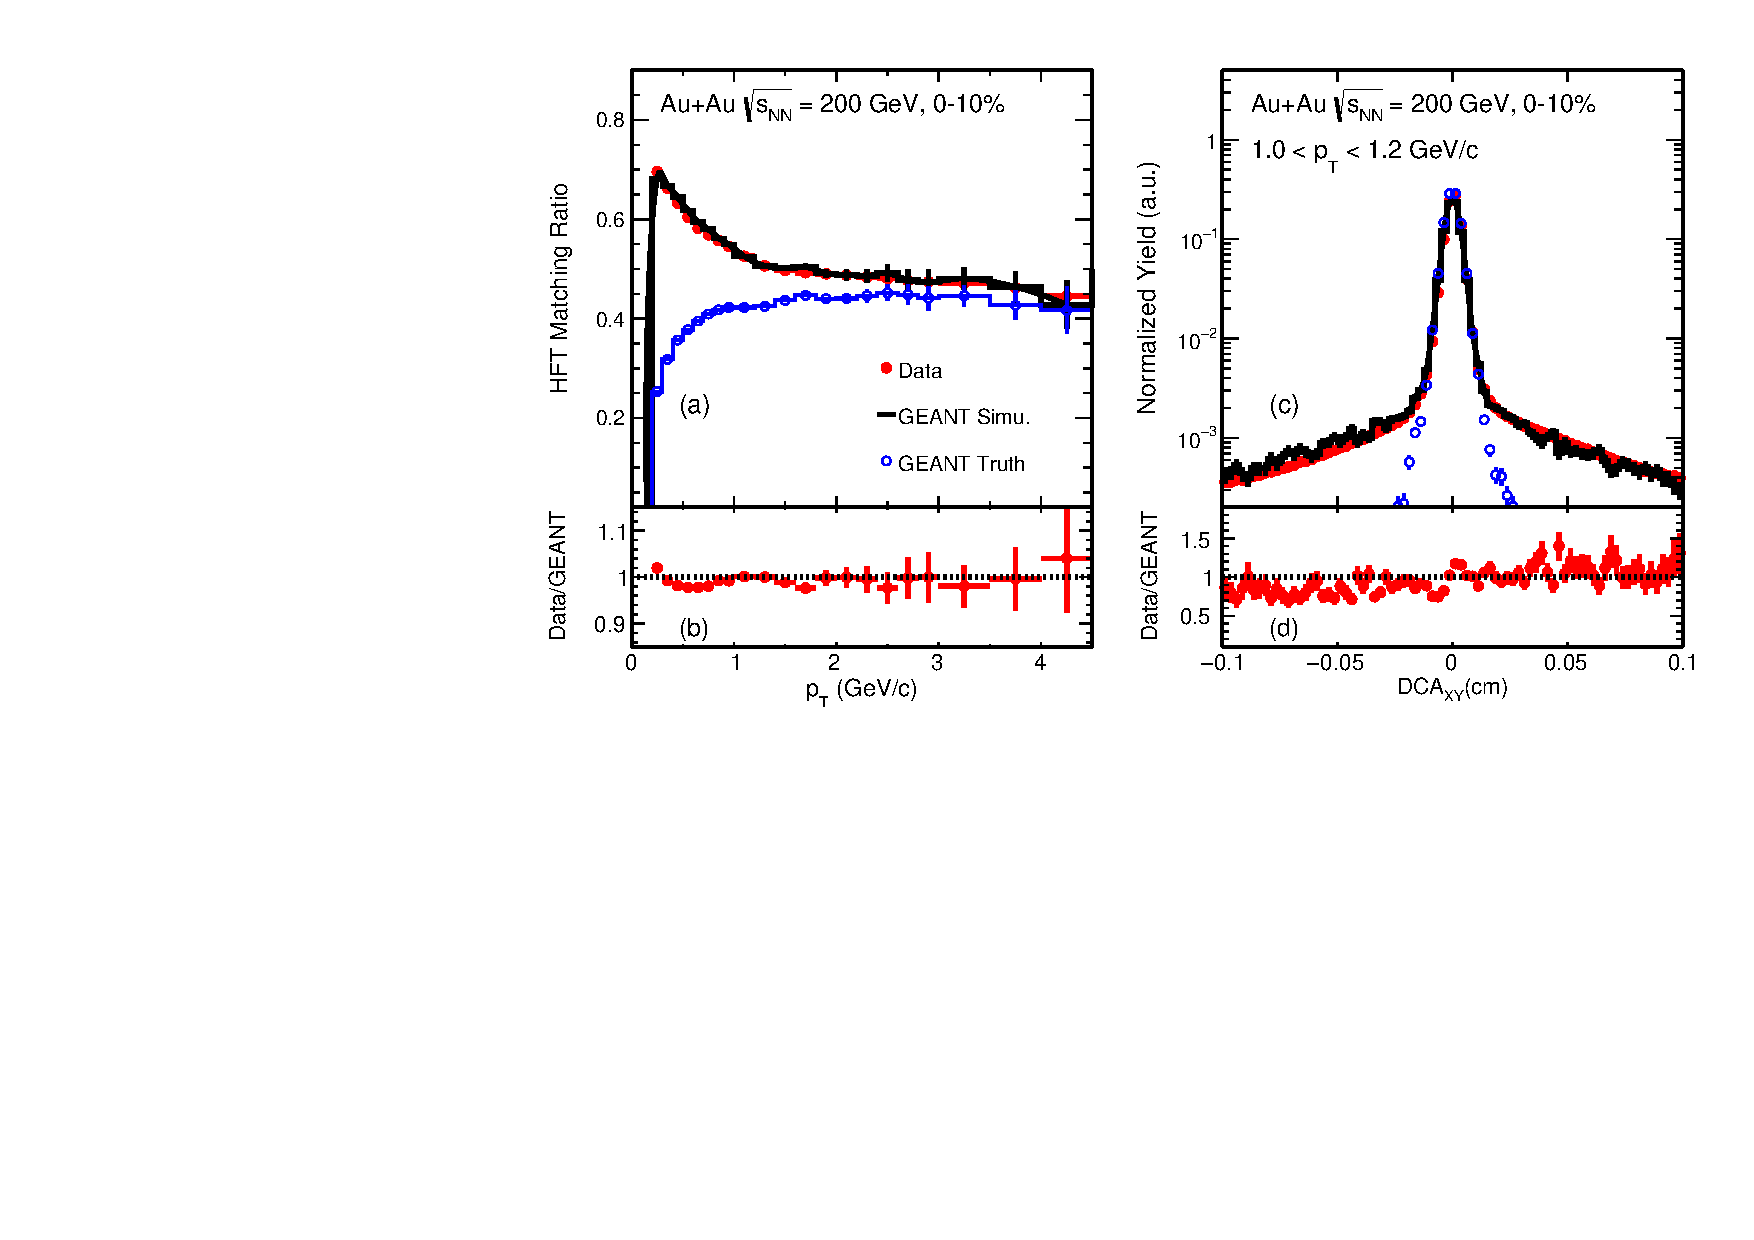
\includegraphics[width=0.85\textwidth]{fig/HijingRatioDca.pdf}
\caption{HFT matching ratio (a) and DCA$_{\rm XY}$ (c) distributions of inclusive charged pions from real data and MC simulation in 0--10\% Au+Au collisions at $\sqrt{s_{_{\rm NN}}}$ = 200\,GeV. The ratios between real data and GEANT simulation are shown in the bottom panels. The blue histogram depicts the true matches in the GEANT simulation.}
\label{fig:HijingRatioDca} 
\end{figure*}

% Effectively, these 1D and 2D histograms encode HFT efficiency, acceptance and spatial resolution performance in Run14 data.

With the tuned simulation setup (with ideal HFT geometry), we use this sample to validate our data-driven simulation approach for $D^0$ efficiency correction calculation. We follow the same procedure as described in Sec.~\ref{sec:correction:hft:fastsim} to obtain the HFT match ratio as well as the 2D $\textup{DCA}_\textup{XY}$-$\textup{DCA}_\textup{Z}$ distributions from the reconstructed data. They are fed into the data-driven simulation to calculate the $D^0$ reconstruction efficiency. This will be compared to the real $D^0$ reconstruction efficiency directly obtained from the GEANT simulation sample.

\begin{figure*}
\centering
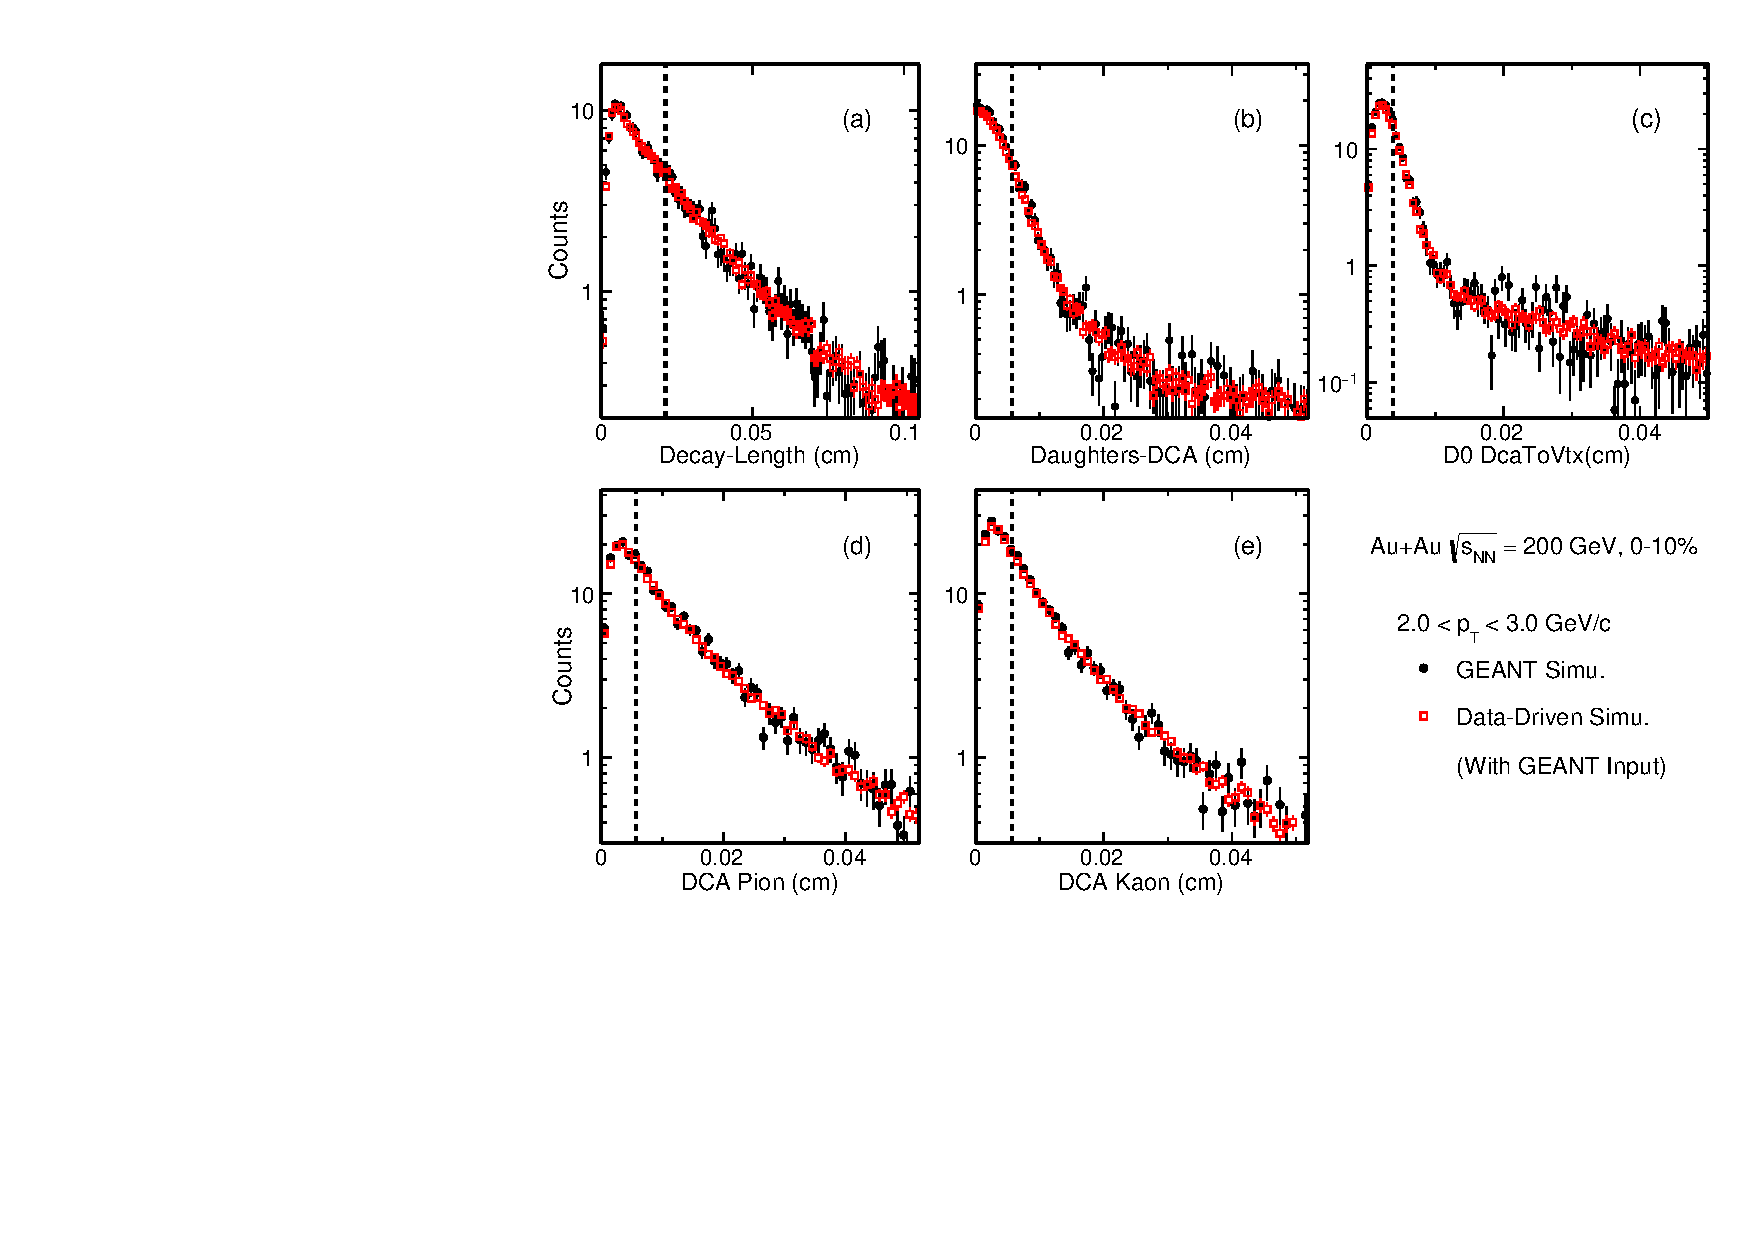
\includegraphics[width=1.0\textwidth]{fig/McTopo.pdf}
\caption{Topological distributions comparison between MC GEANT simulation $(black)$ and data-driven fast simulation with the reconstructed distributions in the simulation sample as the input $(red)$ in most central (0--10\%) Au + Au collisions at $\sqrt{s_{_{\rm NN}}}$ = 200\,GeV.}
\label{fig:McTopo} 
\end{figure*}

\begin{figure}
\centering
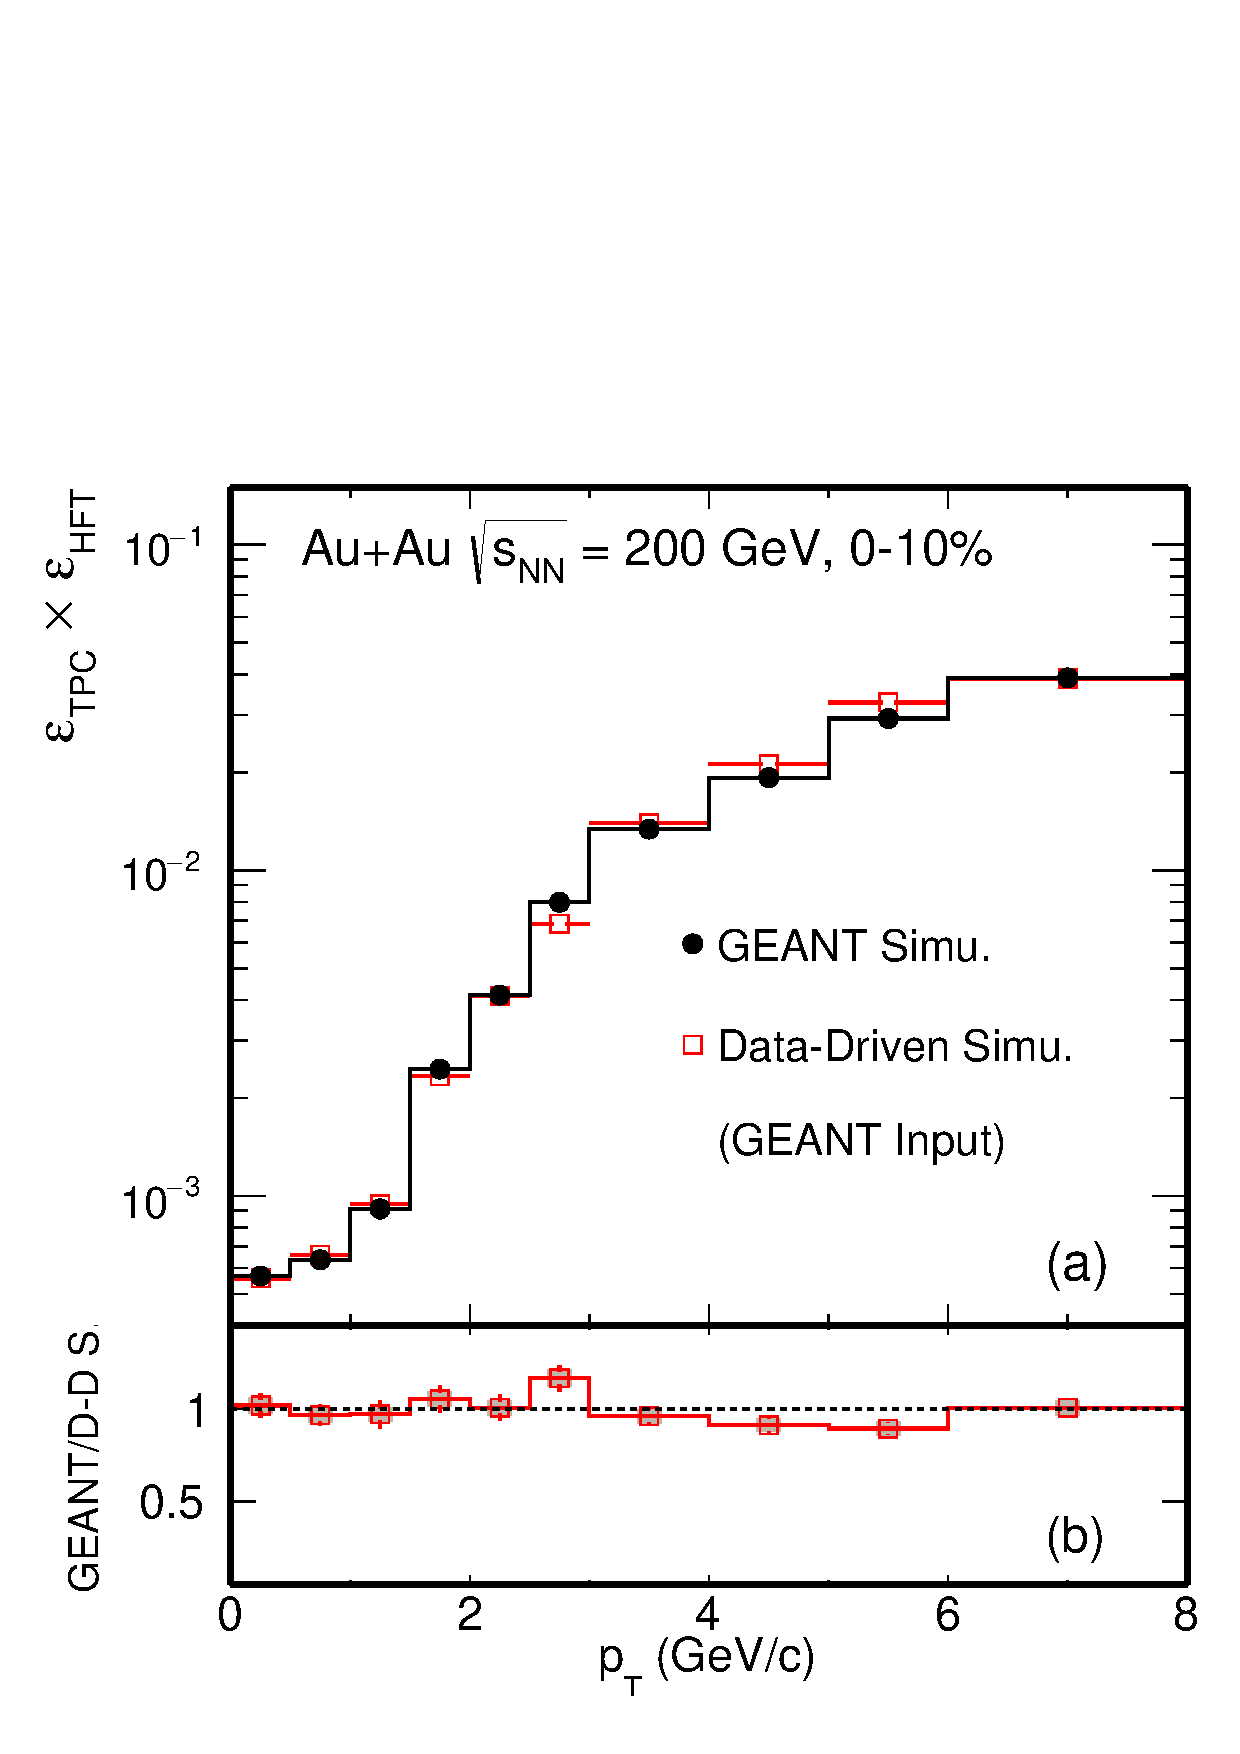
\includegraphics[width=0.43\textwidth]{fig/Mcd0Eff_0_10.pdf}
\caption{$D^{0}$ reconstruction efficiency comparison between MC simulation $(black)$ and data-driven fast simulation with the reconstructed distributions in the simulation sample as the input $(red)$ in central 0-10\% Au + Au collisions at $\sqrt{s_{_{\rm NN}}}$ = 200\,GeV.}
\label{fig:Mcd0Eff_0_10} 
\end{figure}


%Since the MC simulation can describe the data reasonable well, we can use the simulation samples to verify our efficiency correction procedures. The idea is simple, we have this enriched $D^0$ Hijing simulation sample. After run through the detector and full GEANT simulation, the $D^0$ efficiency and topological variables distributions can be extracted. Another procedure is extract the necessary ingredients from this Hijing simulation sample for the Fast-Simulation input (Fast-Simulation with Hijing input), such as the TPC Tracking efficiency, the HFT matching ratio and the 2D $\textup{DCA}_\textup{XY}$-$\textup{DCA}_\textup{Z}$ distributions similar as we used in real data analysis and discussed in the previous section. Then run through the Fast Simulation, as discussed before, the $D^0$ efficiency and topological variables can also extracted in this way and can be compared to the first Hijing + GEANT procedure.

To validate the data-driven simulation tool, Fig.~\ref{fig:McTopo} shows comparisons of several topological variables used in the $D^0$ reconstruction obtained from the GEANT simulation directly and from the data-driven simulation with the reconstructed distributions from the GEANT simulation as the input in the most central (0--10\%) centrality and in 2$<p_{\rm T}<$3\,GeV/$c$. The topological variables shown here are $D^0$ decay length, DCA between two $D^0$ decay daughters, $D^0$ DCA with respect to the collision vertex, pion DCA and kaon DCA with respect to the collision vertex. As seen in this figure, the data-driven simulation tool reproduces all these topological distributions quite well.

Figure~\ref{fig:Mcd0Eff_0_10} shows the $D^0$ reconstruction efficiency $\varepsilon_{\rm TPC}\times\varepsilon_{\rm HFT}$ from the following two methods in this simulation. The first method is the standard calculation by applying the tracking and topological cuts for reconstructed $D^0$ mesons in this simulation sample. In the second method, we employ the data-driven simulation method and take the reconstructed distributions from this simulation sample as the input and then calculate the $D^0$ reconstruction efficiency in the data-driven simulation framework. In panel (a) of Fig.~\ref{fig:Mcd0Eff_0_10}, efficiencies from two calculation methods agree well in the $p_{\rm T}$ bins in central 0--10\% Au+Au collisions at $\sqrt{s_{_{\rm NN}}}$ = 200\,GeV, and the ratio between the two is shown in panel (b). This demonstrates that the data-driven simulation tool can reproduce well the real $D^0$ reconstruction efficiency in central Au+Au collisions.

% \begin{figure*}
% \centering
% 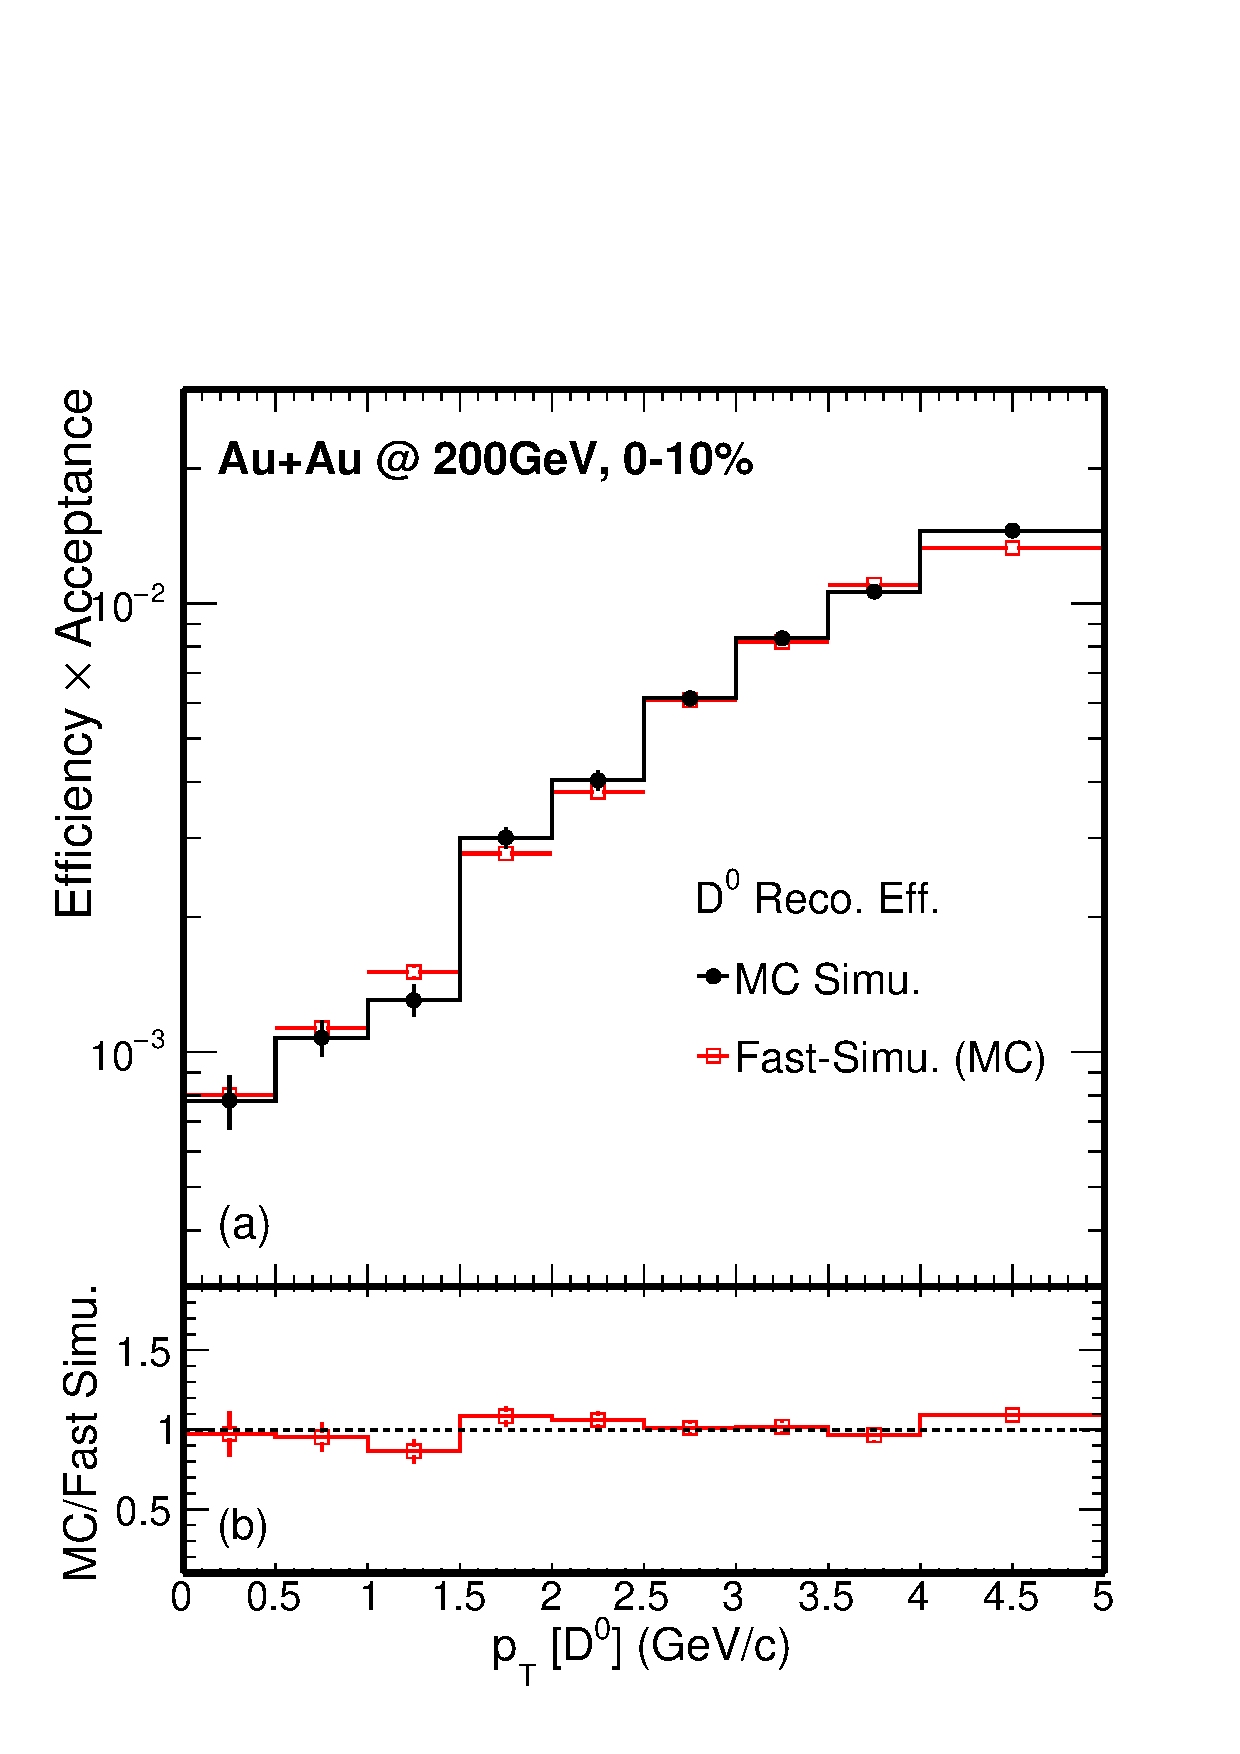
\includegraphics[width=0.45\textwidth]{fig/Mcd0Eff.pdf}
% \caption{$D^{0}$ reconstruction efficiency comparison between MC simulation $(black)$ and Fast-Simulation rely on MC simulation as input $(red)$ in most central Au + Au collisions.}
% \label{fig:Mcd0Eff} 
% \end{figure*}

\subsubsection{\label{sec:correction:hft:fordata}Efficiency for real data}

\begin{figure*}
\centering
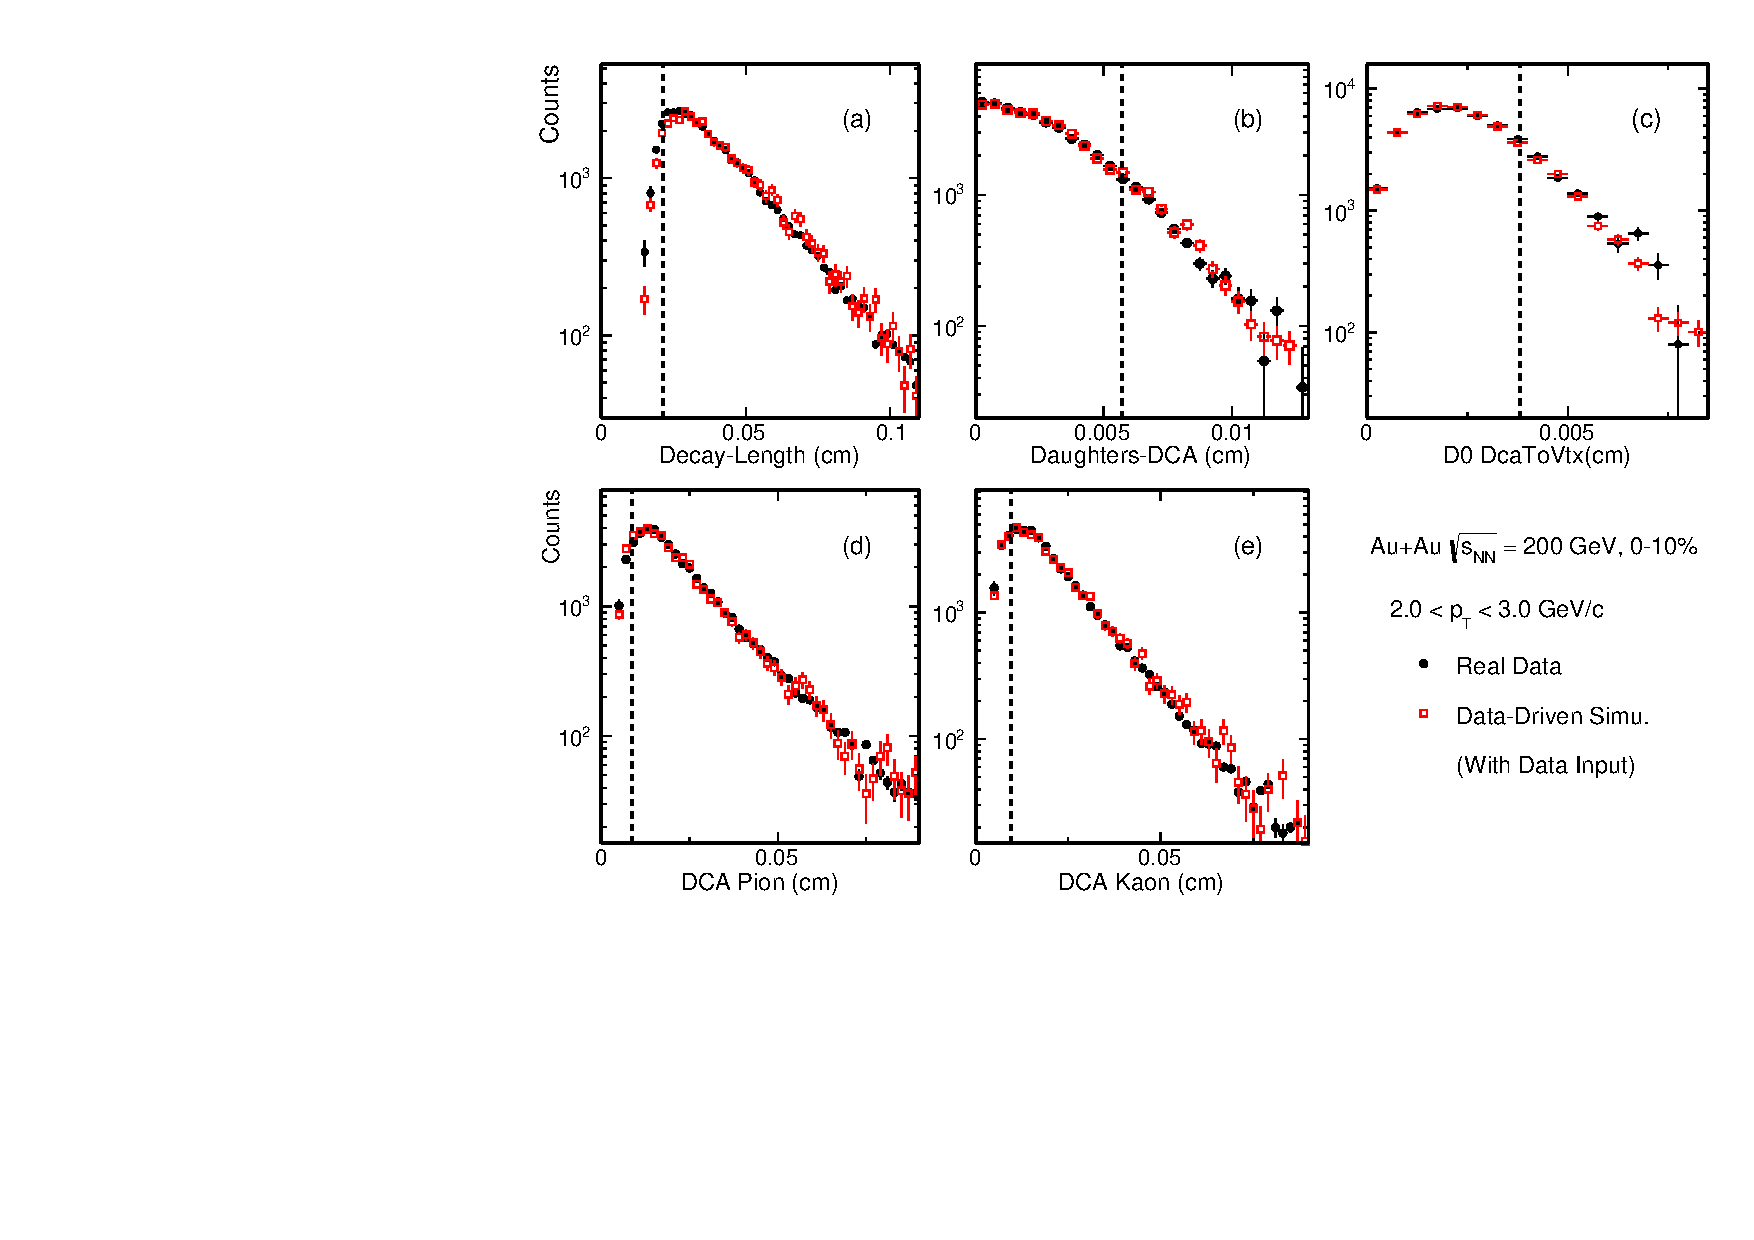
\includegraphics[width=1.0\textwidth]{fig/DataTopo.pdf}
\caption{Comparison of topological variable distributions between $D^0$ signals in real data $(black)$ and in data-driven Simulation with real data distributions as the input $(red)$ in most central (0--10\%) Au + Au collisions at $\sqrt{s_{_{\rm NN}}}$ = 200\,GeV. The dashed lines indicate the final topological cuts chosen for each individual topological variable.}
\label{fig:DataTopo} 
\end{figure*}

We employ the validated data-driven simulation method for the real data analysis. Fig.~\ref{fig:DataTopo} shows the comparisons of the same five topological variables between $D^0$ signals in real data and data-driven simulated distributions with real data as the input in central 0--10\% collisions for $D^0$ at 2$<p_{\rm T}<$3\,GeV/$c$. The real data distributions are extracted by reconstructing the $D^0$ signal with initial cuts and then statistically subtracting the background distributions using the side-band method. The initial cuts are necessary here to ensure reasonable $D^0$ signal reconstruction for the extraction of these topological variable distributions, while these pre-cuts effectively reduce the low end reach for several topological variables, e.g. the $D^0$ decay length. In the data-driven simulation method, charged pion and kaon HFT matching ratio and 2D DCA distributions are used as the input to calculate these topological variables for $D^0$ signals. Fig.~\ref{fig:DataTopo} shows that in the selected ranges, the data-driven simulation method reproduces well topological variables distributions of $D^0$ signals, which supports that this method can be reliably used to calculate the topological cut efficiency.

\begin{figure}[h]
\centering
% 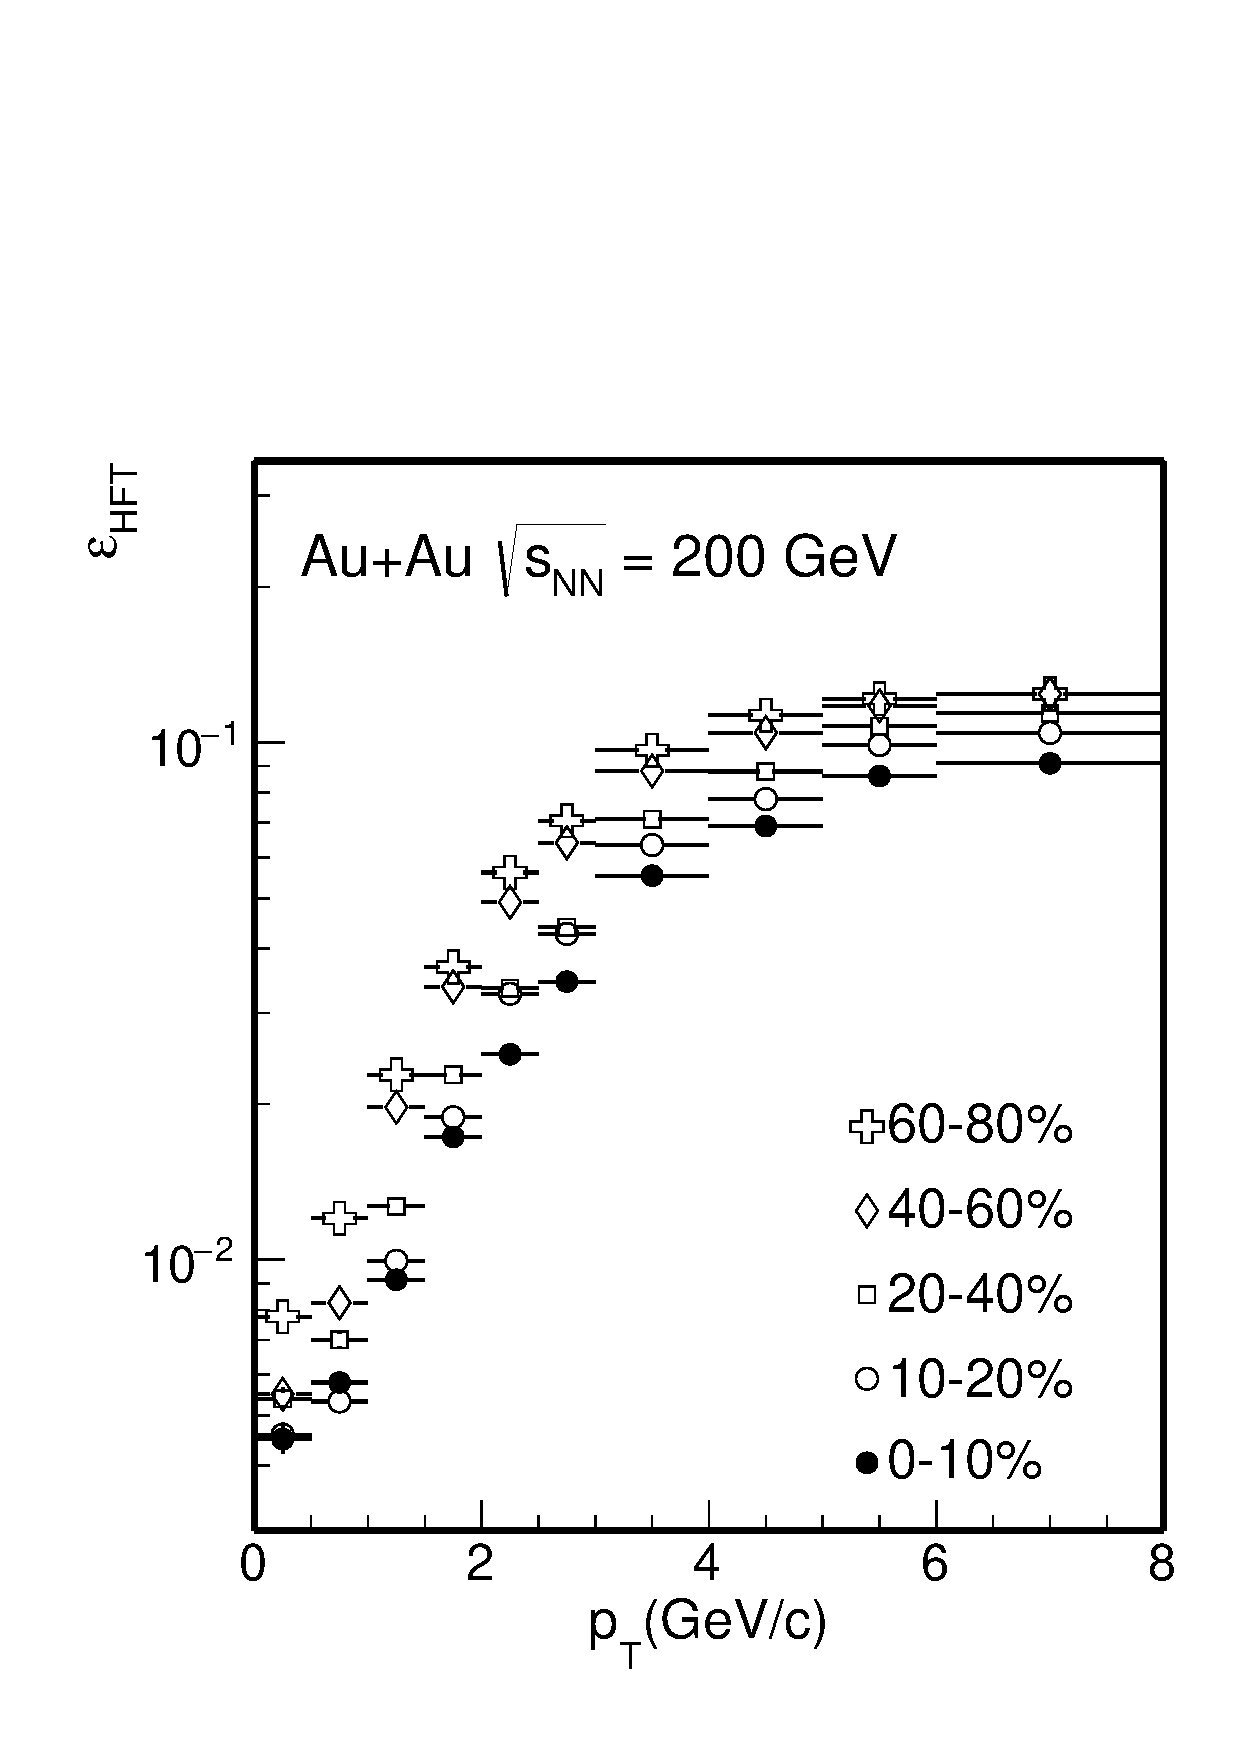
\includegraphics[width=0.4\textwidth]{fig/Datad0Eff_hftTopo.pdf}
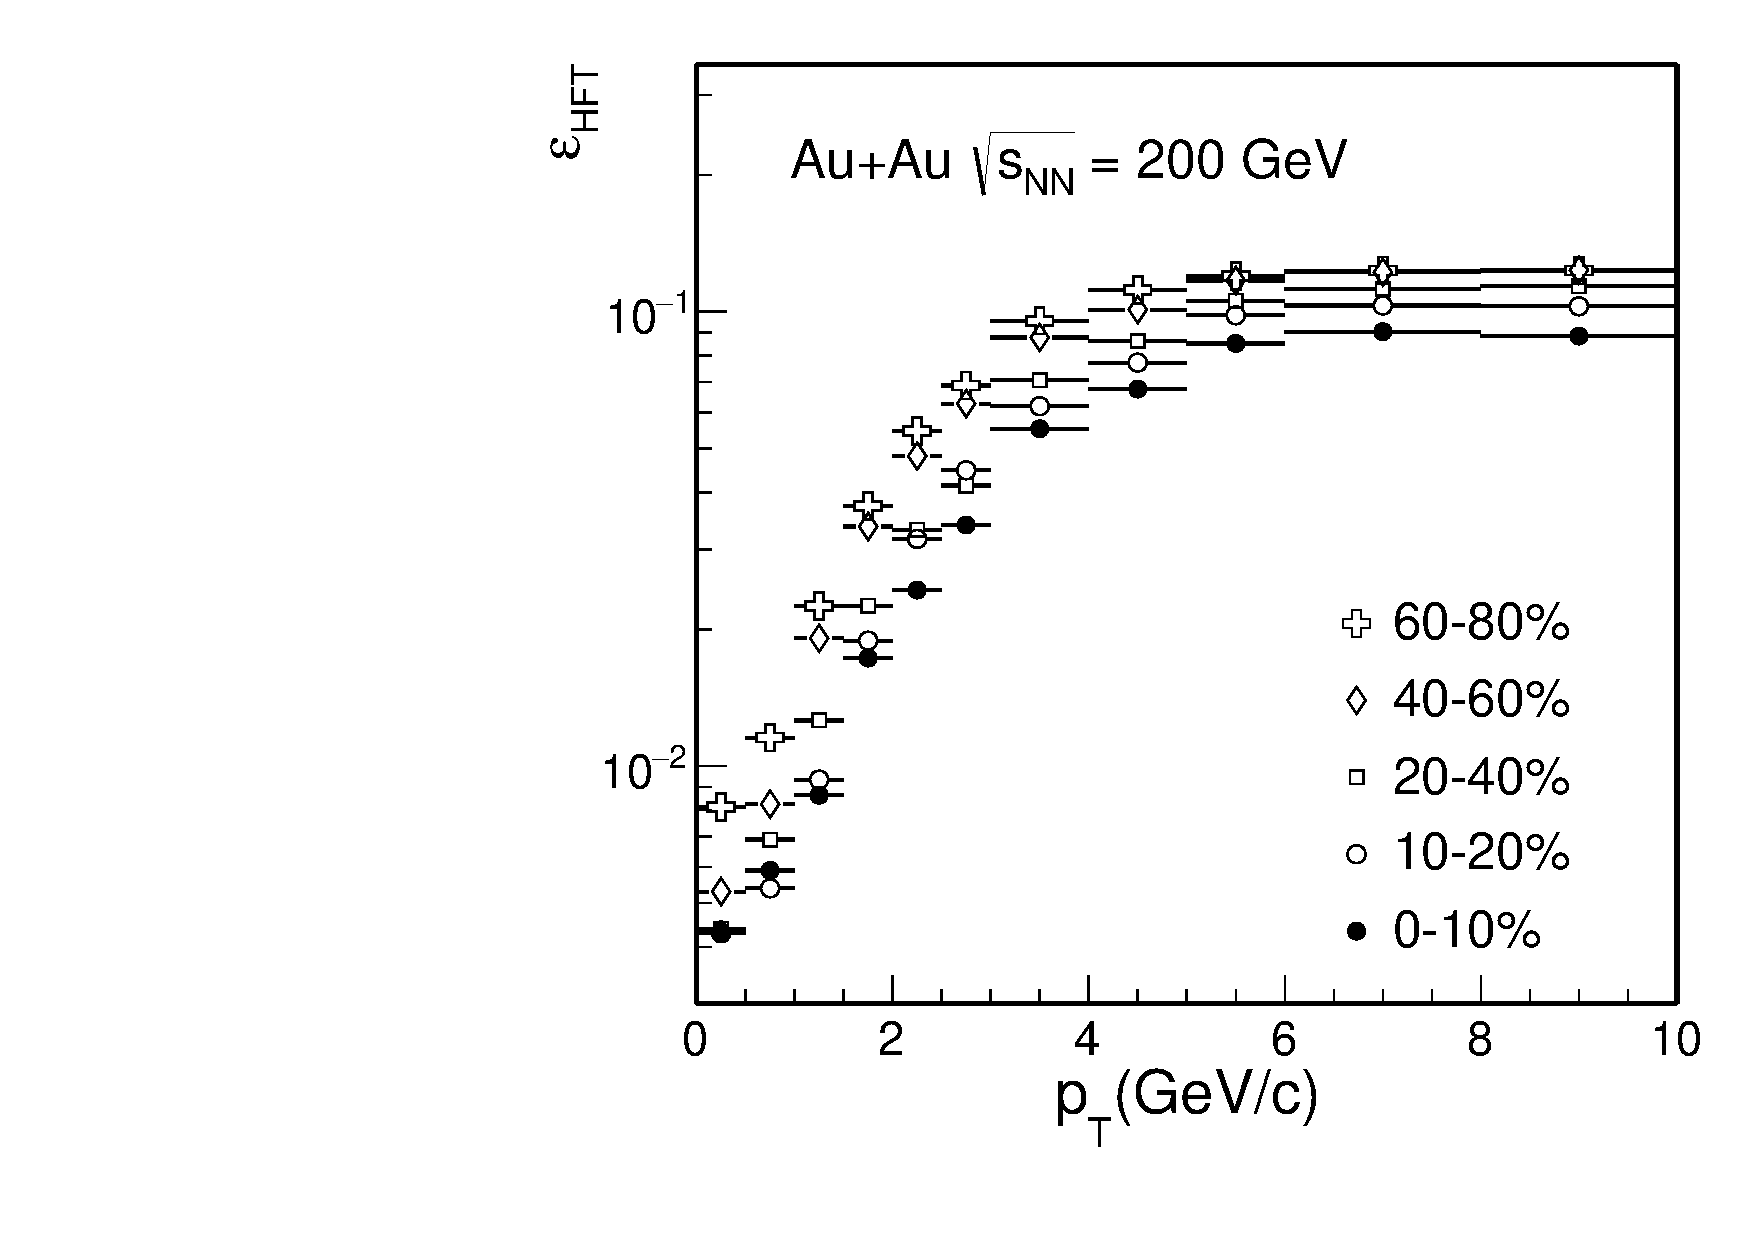
\includegraphics[width=0.43\textwidth]{fig/Datad0Eff_hftTopo_10.pdf}
\caption{$D^{0}$ HFT tracking and topological cut efficiencies from different centrality classes in Au + Au collisions at $\sqrt{s_{_{\rm NN}}}$ = 200\,GeV.}
\label{fig:Datad0Eff_hftTopo} 
\end{figure}


Figure~\ref{fig:Datad0Eff_hftTopo} shows the HFT tracking and topological cut efficiency $\varepsilon_{\rm HFT}$ as a function of $D^0$ $p_{\rm T}$ for different centrality bins obtained using the data-driven simulation method described in this section using the input distributions from real data. The smaller efficiency seen in central collisions is in part because the HFT tracking efficiency is lower in higher occupancy central collisions, and in addition because we choose tighter topological cuts in central collisions for background suppression.

\subsubsection{\label{sec:correction:hft:secondary}Secondary particle contribution}

\begin{figure}[h]
\centering
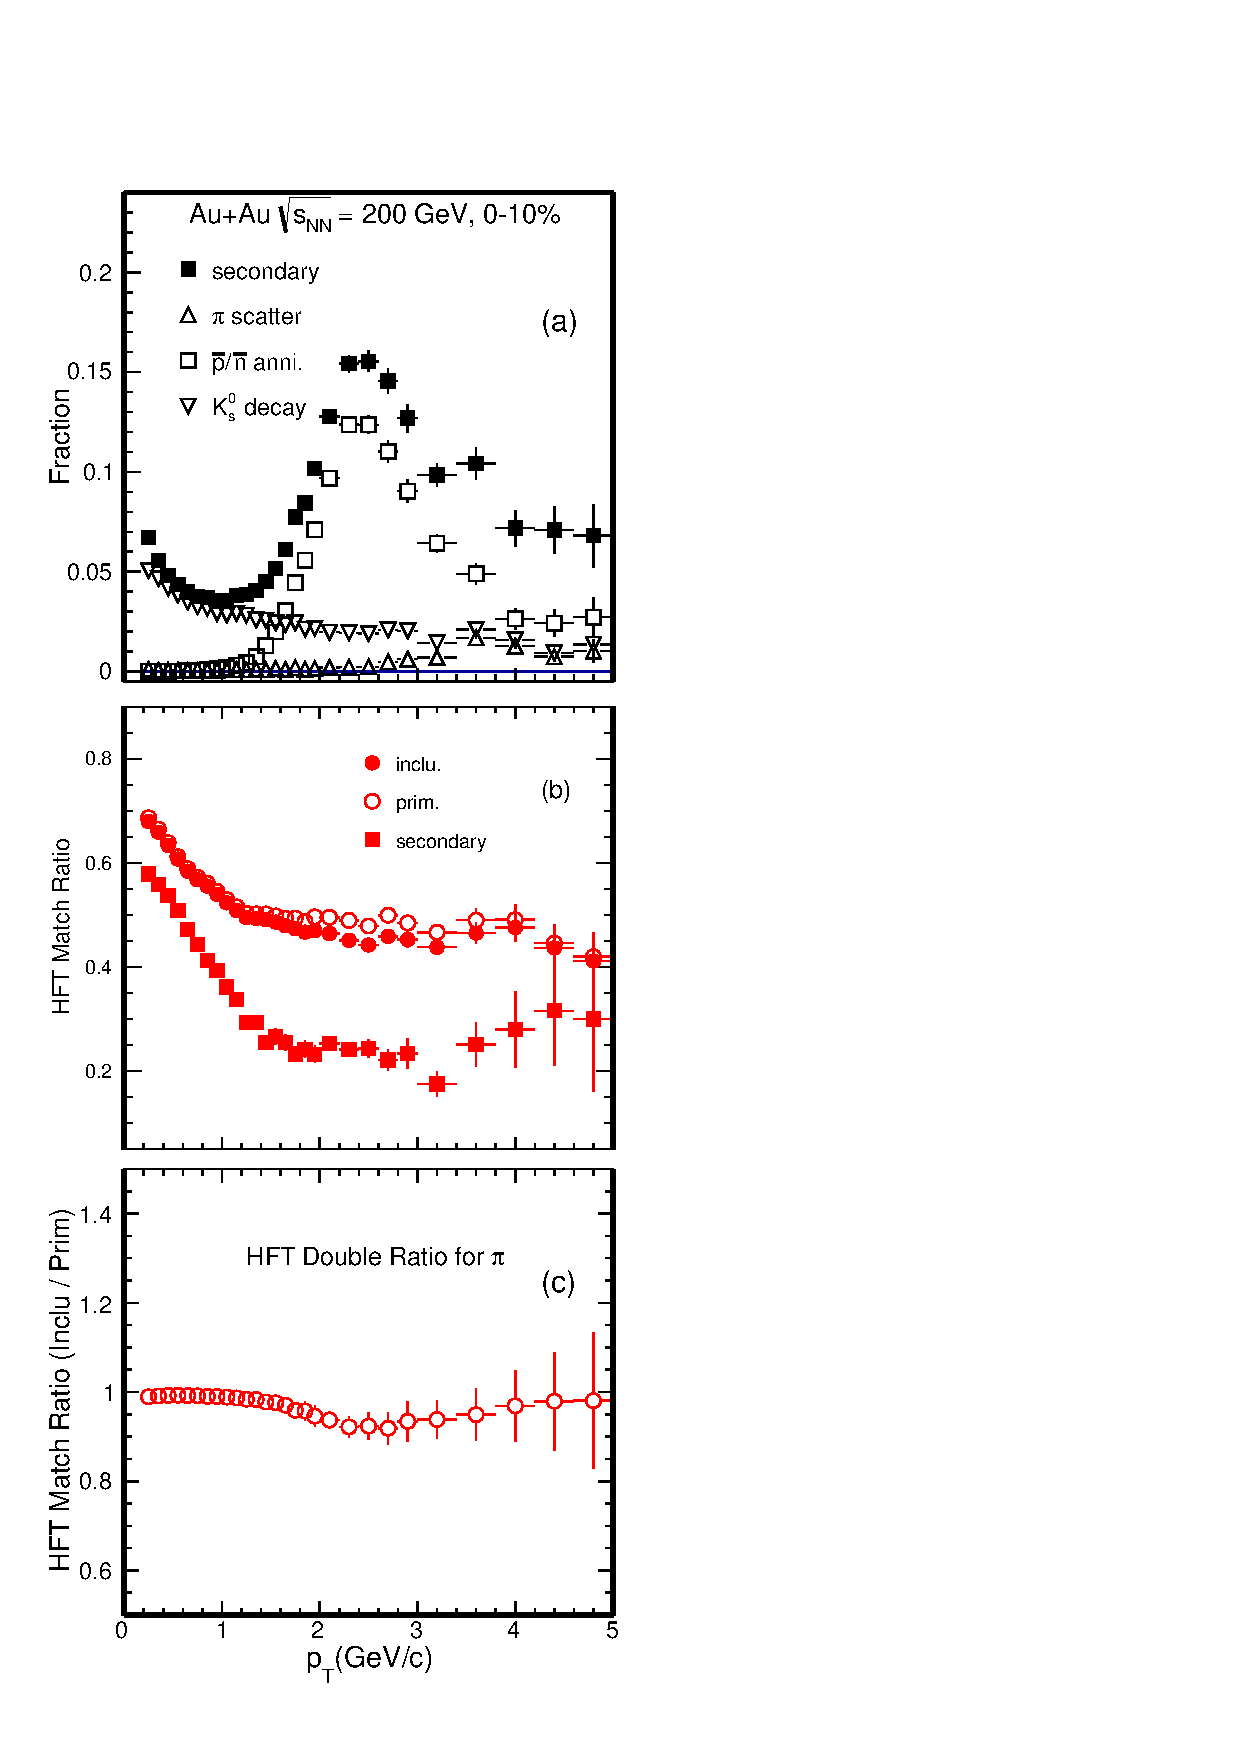
\includegraphics[width=0.41\textwidth, angle = 0]{fig/Fraction_Pion.pdf}
\caption{Secondary pion contribution in Au + Au collisions at $\sqrt{s_{_{\rm NN}}}$ = 200\,GeV. Panel (a) shows the fraction of different sources for secondary tracks. Panel (b) shows the HFT match ratio while panel (c) shows the HFT match double ratio which divide the inclusive one to the primary ones.}
\label{fig:Fraction_Pion} 
\end{figure}

In the data-driven method for obtaining the efficiency correction, inclusive pion and kaon distributions are taken from real data as the input. There is a small amount of secondary contribution (e.g. weak decays from $K^0_S$ and $\Lambda$) to the measured charged pion tracks.

The impact of secondary particle contribution to the charged pions is studied using the Hijing events processed through the GEANT simulation and the same offline reconstruction. The fraction of secondary pions from weak decay of strange hadrons ($K^0_S$ and $\Lambda$) to the total inclusive charged pions within ${\rm DCA}<$ 1.5\,cm cut is estimated to be around 5\% at pion $p_{\rm T}$ = 0.3\,GeV/$c$ and decrease to be $<2\%$ above 2\,GeV/$c$. This is consistent with what is observed before in measuring the prompt charged pion spectra~\cite{Adams:2003xp}. There is another finite contribution of low momentum anti-protons and anti-neutrons annihilated in the detector material and producing secondary pions. The transverse momenta of these pions are mostly around 2--3\,GeV/$c$ and the fraction of total inclusive pions is $\sim$ 10--12\% at $p_{\rm T}=$ 2--3\,GeV/$c$ based on this simulation and contribute $\sim$ 5--8\% to the HFT matching ratio. This was obtained using the GEANT with GHEISHA hadronic package. With a difference hadronic package, FLUKA, the secondary pion fraction in 2--3\,GeV/$c$ region is significantly reduced to be negligible. The difference between the primary pions and the inclusive pions in the HFT matching ratio has been considered as one additional correction factor to take into account these secondary pions in our data-driven simulation method when calculating the efficiency correction, while the maximum difference with respect to the result obtained using the GHEISHA hadronic package is included as the systematic uncertainty for this source.  Fig.~\ref{fig:Fraction_Pion} shows the secondary pion contribution in Au + Au collisions at $\sqrt{s_{_{\rm NN}}}$ = 200\,GeV. Panel (a) shows the fraction of different sources for secondary tracks including the weak decays, the scatters and the annihilation. Panel (b) shows the different contributions to the HFT match ratio while panel (c) is the HFT match double ratio which divide the inclusive one to the primary ones. The effect of such secondary contribution to charged kaons is negligible~\cite{Adams:2003xp}.

\subsection{\label{sec:correction:vtx}Vertex Resolution Correction - $\varepsilon_{\rm vtx}$}

In the data-driven approach, $D^0$ mesons are injected at event primary vertex. In the real data, reconstructed vertex may have finite resolution with respect to real collision vertex. This may have sizable impact on the reconstructed $D^0$ signal counts after applying the topological cuts in small multiplicity events where the event vertex resolution becomes large. Fig.~\ref{fig:vtxX_vsCent} shows the Full-Width-at-Half-Maximum (FWHM) of the difference in a vertex x-position of two randomly-divided sub-events in various centrality bins. We choose the FWHM variable here as the distributions are not particularly Gaussian.

\begin{figure}
\centering
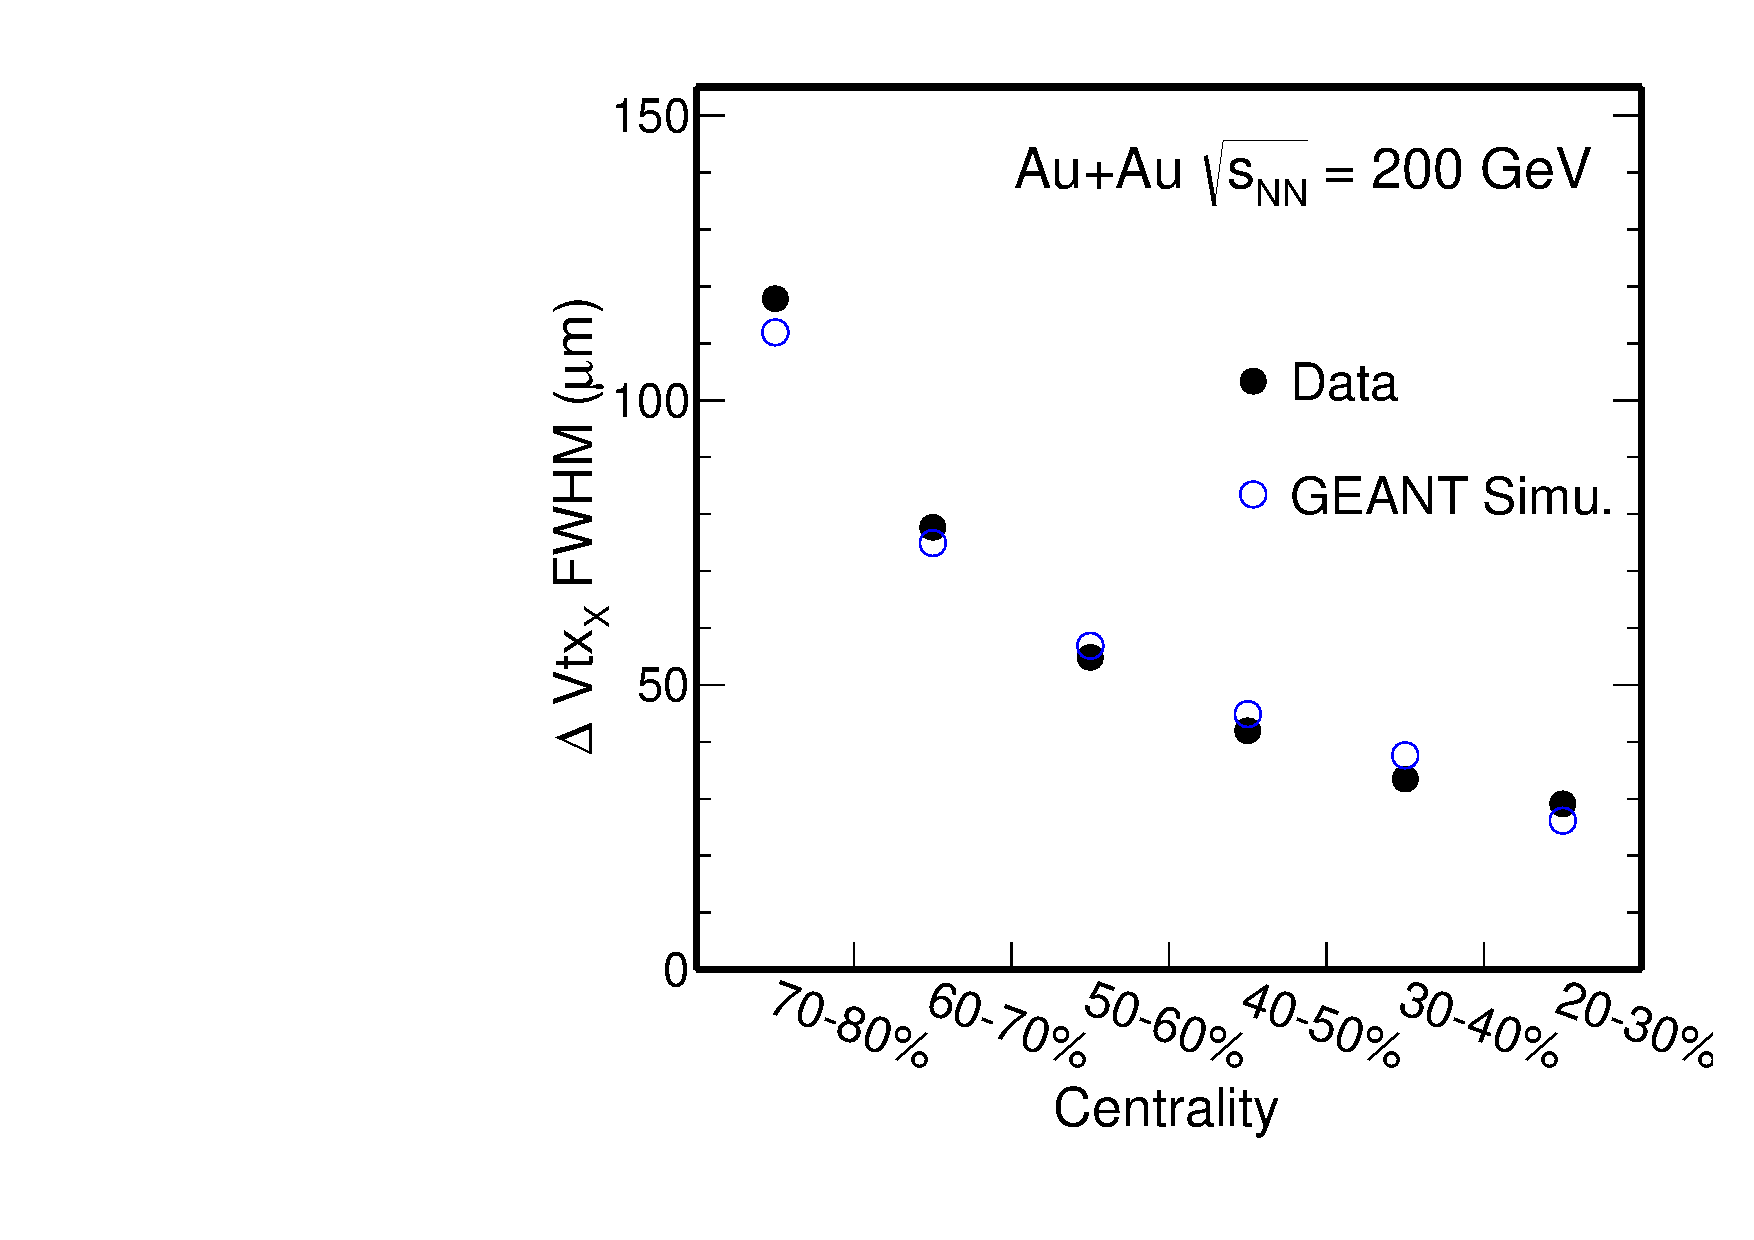
\includegraphics[width=0.41\textwidth]{fig/vtxX_vsCent.pdf}
\caption{Full-Width-at-Half-Maximum (FWHM) of vertex position difference in the X dimension between two randomly-divided sub-events in various centrality bins in Au + Au collisions. Black solid circles present the FWHM from real data while the blue empty circles are GEANT simulation.}
\label{fig:vtxX_vsCent} 
\end{figure}

The MC simulation reproduces the vertex difference distributions seen in the real data reasonably well. This gives us confidence in using this MC simulation setup to evaluate the vertex resolution correction $\varepsilon_{\rm vtx}$.

\begin{figure*}
\centering
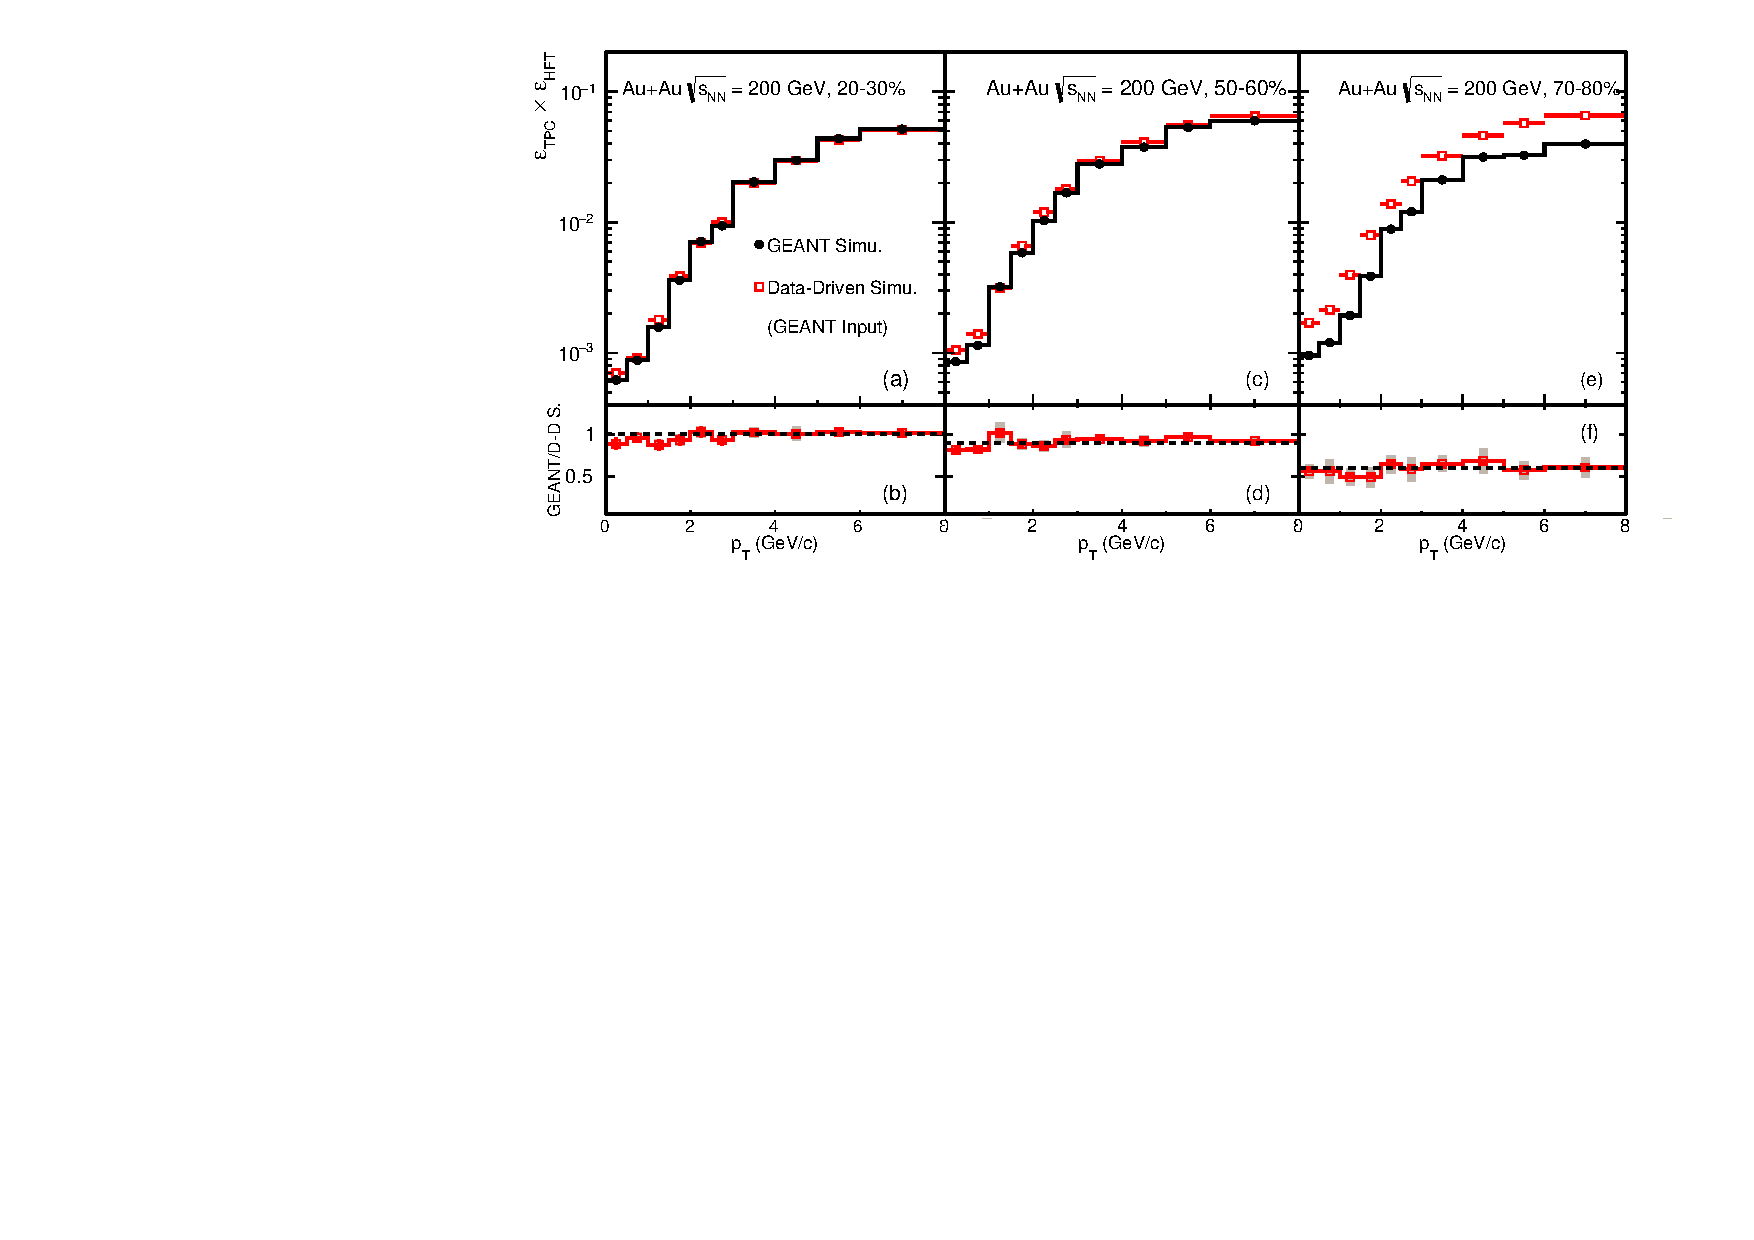
\includegraphics[width=1.05\textwidth]{fig/Mcd0Eff_20_80.pdf}
\caption{$D^{0}$ reconstruction efficiency comparison between MC GEANT simulation $(black)$ and  data-driven simulation with the reconstructed distributions in the simulation as the input $(red)$ for 20--30\% (left), 50--60\% (middle) and 70--80\% (right) Au + Au collisions at $\sqrt{s_{_{\rm NN}}}$ = 200\,GeV.}
\label{fig:Mcd0Eff_20_80} 
\end{figure*}

\begin{figure}
\centering
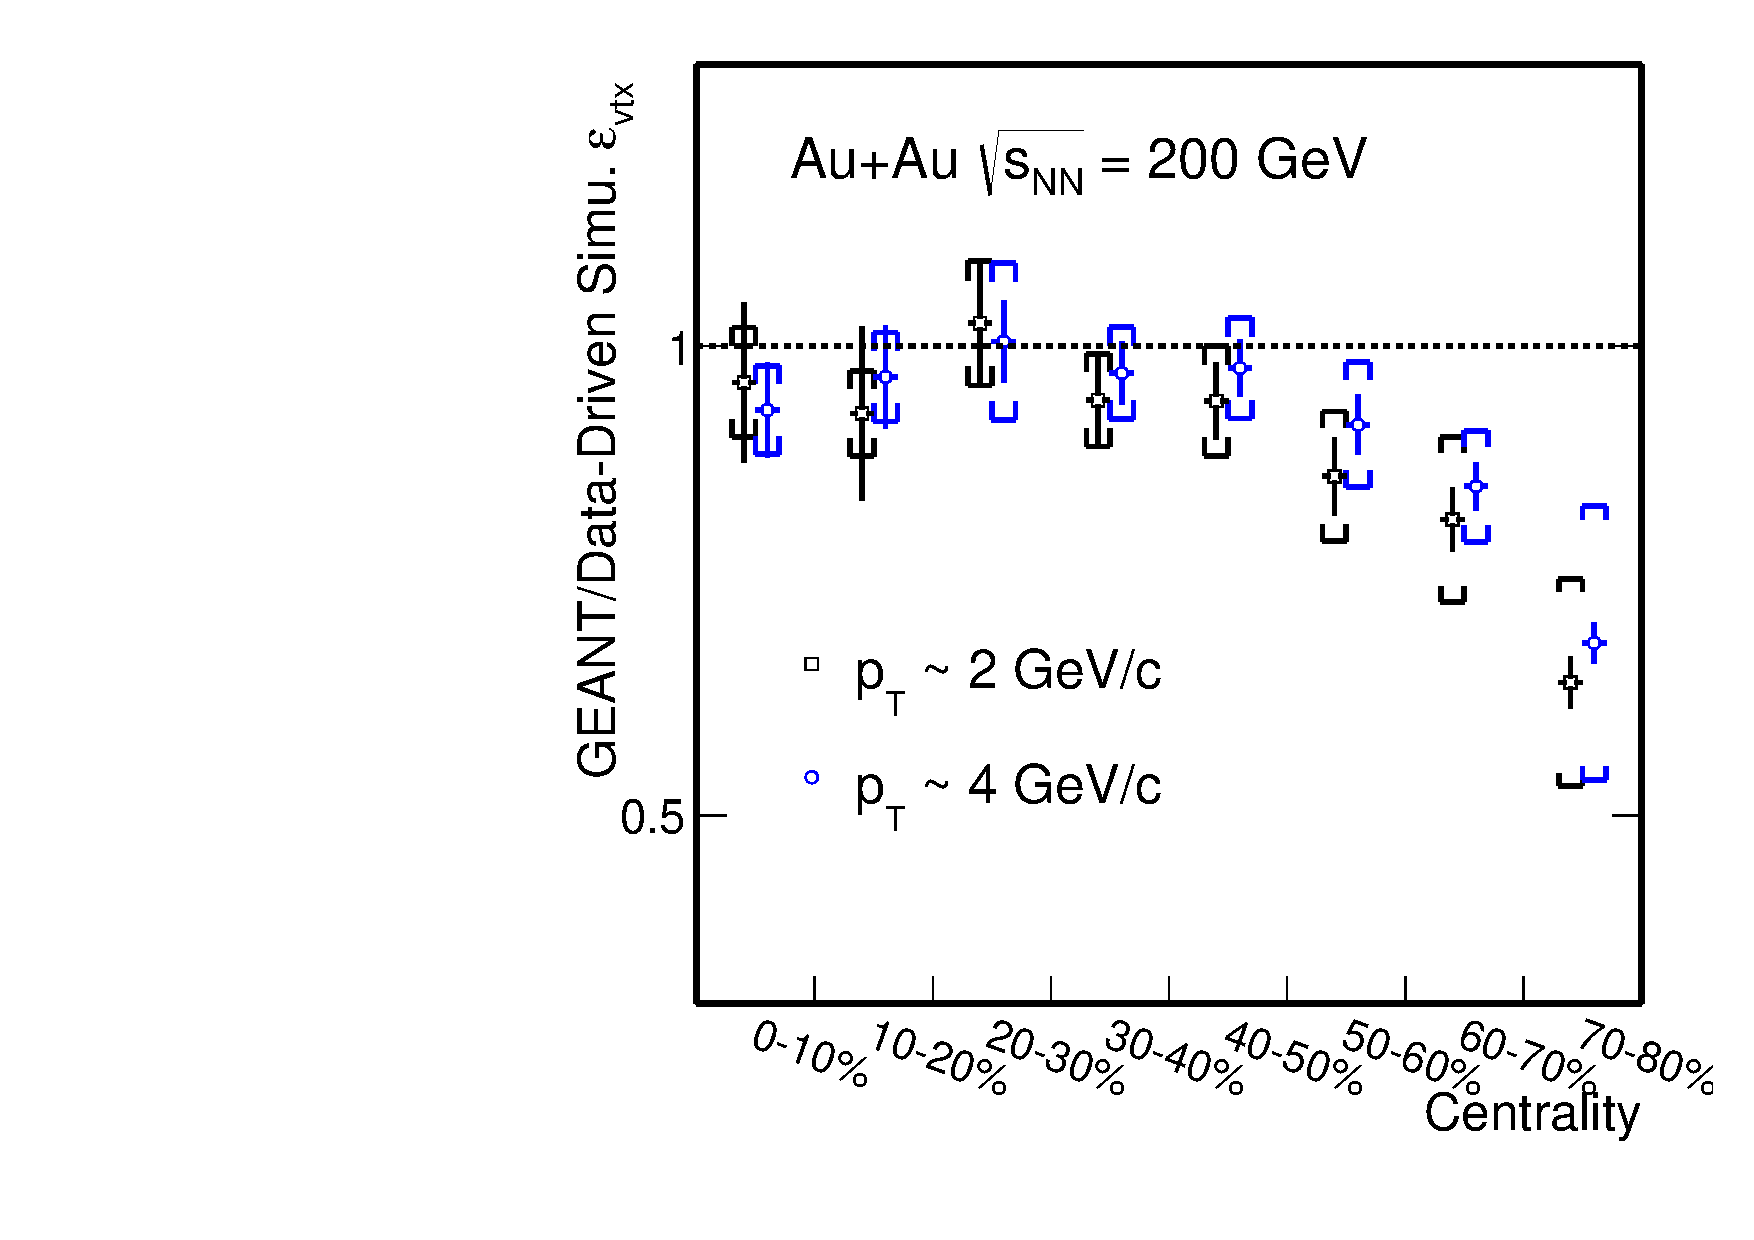
\includegraphics[width=0.43\textwidth]{fig/Mcd0Eff_20_80_vsCent.pdf}
\caption{$\varepsilon_{\rm vtx}$, $D^0$ reconstruction efficiency ratios between MC GEANT simulation and data-driven simulation with the reconstructed distributions in the simulation as the input versus collision centrality in Au + Au collisions for $p_{\rm T}$ at 2 and 4\,GeV/$c$. The brackets depict the estimated systematic uncertainties.}
\label{fig:Mcd0Eff_20_80_vsCent} 
\end{figure}

To estimate the vertex resolution effect, we embedded a PYTHIA $c\bar{c}$ event into a Hijing Au+Au event, and ran through the STAR GEANT simulation followed by the same offline reconstruction as in the real data production. The PYTHIA $c\bar{c}$ events are pre-selected to have at least one $D^0\rightarrow K^-\pi^+$ decay or its charge conjugate to enhance the statistics. Figure~\ref{fig:Mcd0Eff_20_80} shows the comparison in the obtained $D^0$ reconstruction efficiency between MC simulation $(black)$ and data-driven simulation using reconstructed distributions in the same MC sample as input $(red)$ for 20--30\%(left), 50--60\%(middle) and 70--80\%(right) centrality bins, respectively. The bottom panels show the ratios of the efficiencies obtained from the two calculation methods. In the central and mid-central collisions, the data-driven simulation method can well reproduce the $D^0$ real reconstruction efficiency. This is as expected since the vertex resolution is small so that it has less impact in the obtained efficiency using the data-driven simulation method. However, in more peripheral collisions, the data-driven simulation method underestimates the $D^0$ reconstruction efficiency as shown in the middle and right panels. The ratio between the two methods, the vertex resolution correction factor $\varepsilon_{\rm vtx}$ denoted in Equ.~\ref{equ:invariantyield}, has a mild $p_{\rm T}$ dependence, but shows a strong centrality dependence shown in Fig.~\ref{fig:Mcd0Eff_20_80_vsCent}, which is the $\varepsilon_{\rm vtx}$ correction factor along different centralities for $p_T$ around 2 and 4 GeV/$c$. The brackets denote the systematic uncertainties in the obtained correction factor $\varepsilon_{\rm vtx}$. They are estimated by tuning the Hijing + GEANT simulation so that the sub-event vertex difference distributions in the real data can be covered by distributions obtained from different simulation samples. The vertex resolution corrections are applied in each individual centralities along with the $p_T$ dependence.

\subsection{\label{sec:correction:PID}PID Efficiency - $\varepsilon_{\rm PID}$ and Doubly-mis-PID Correction}

\begin{figure}
\centering
% 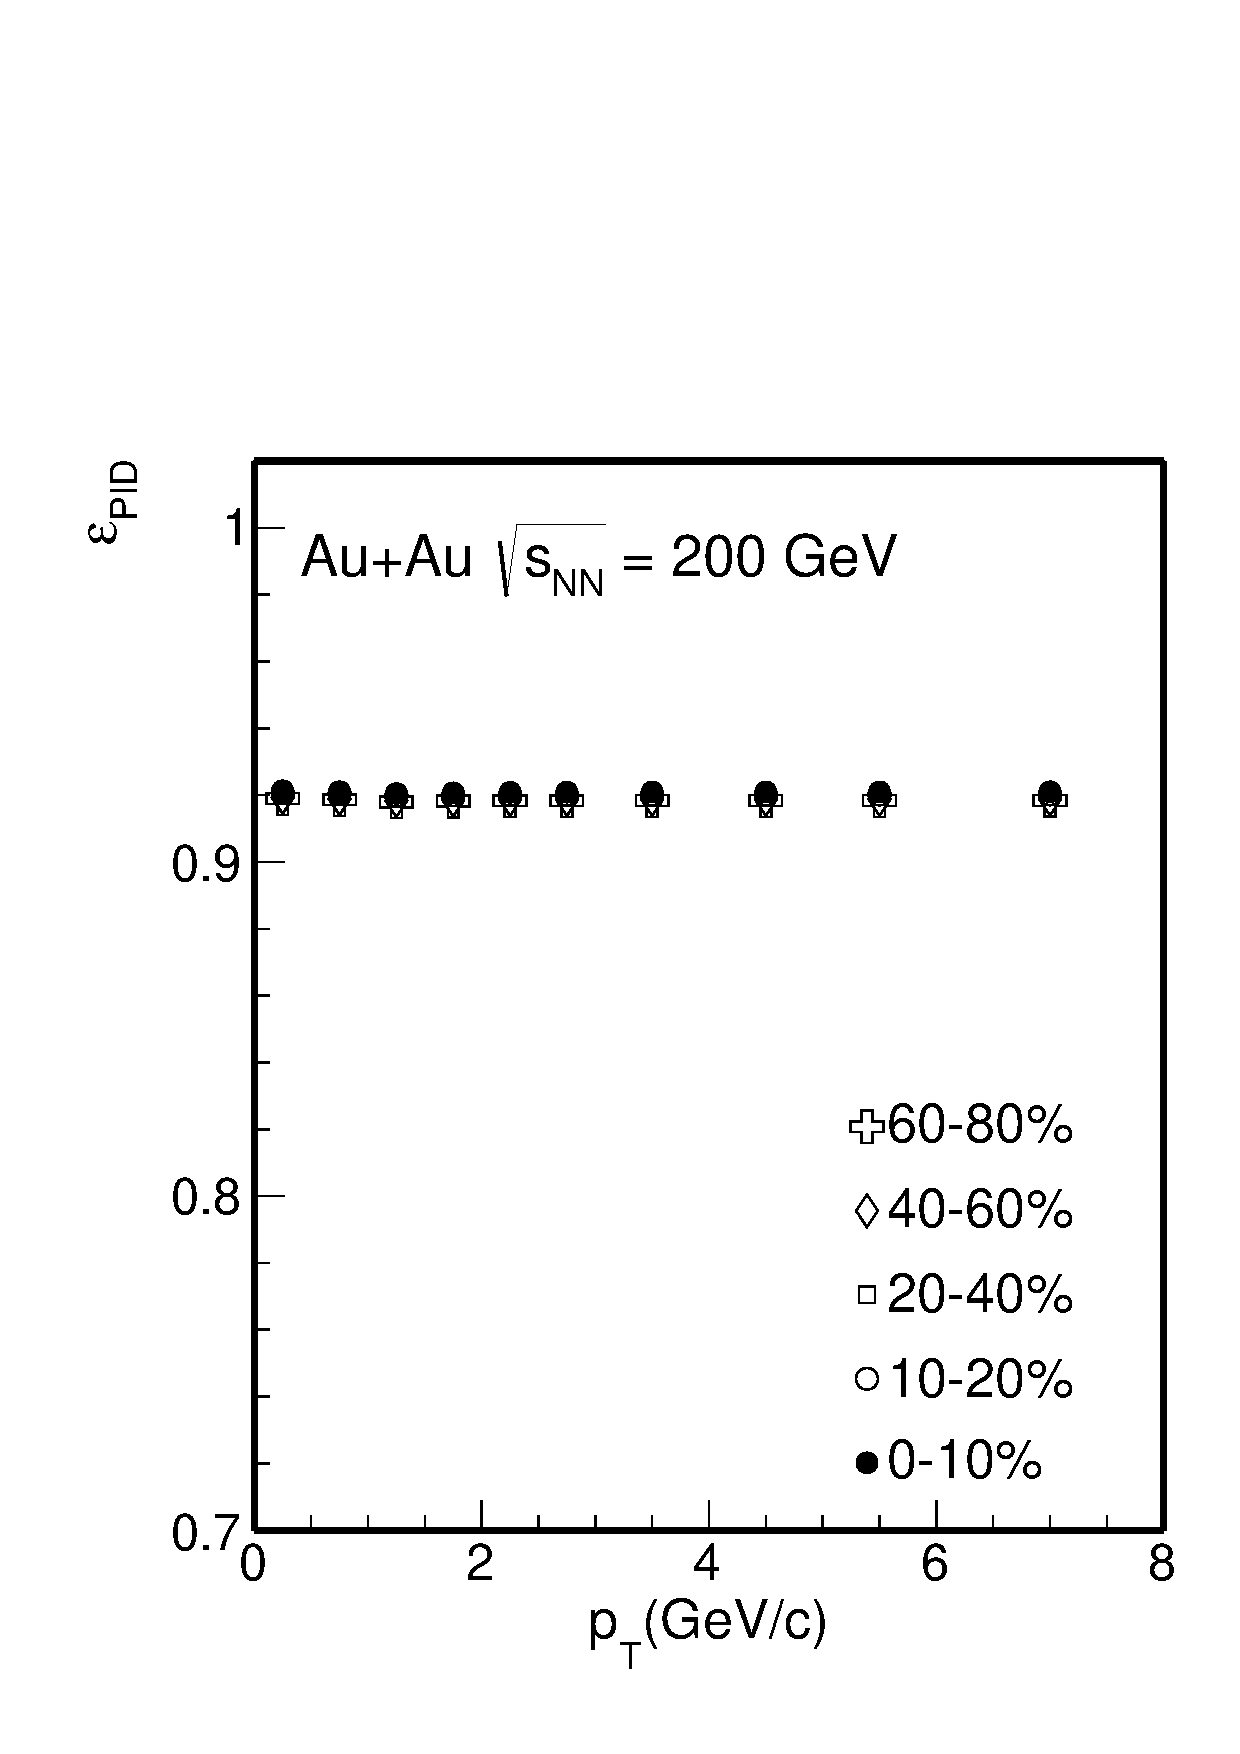
\includegraphics[width=0.4\textwidth]{fig/Datad0Eff_pid.pdf}
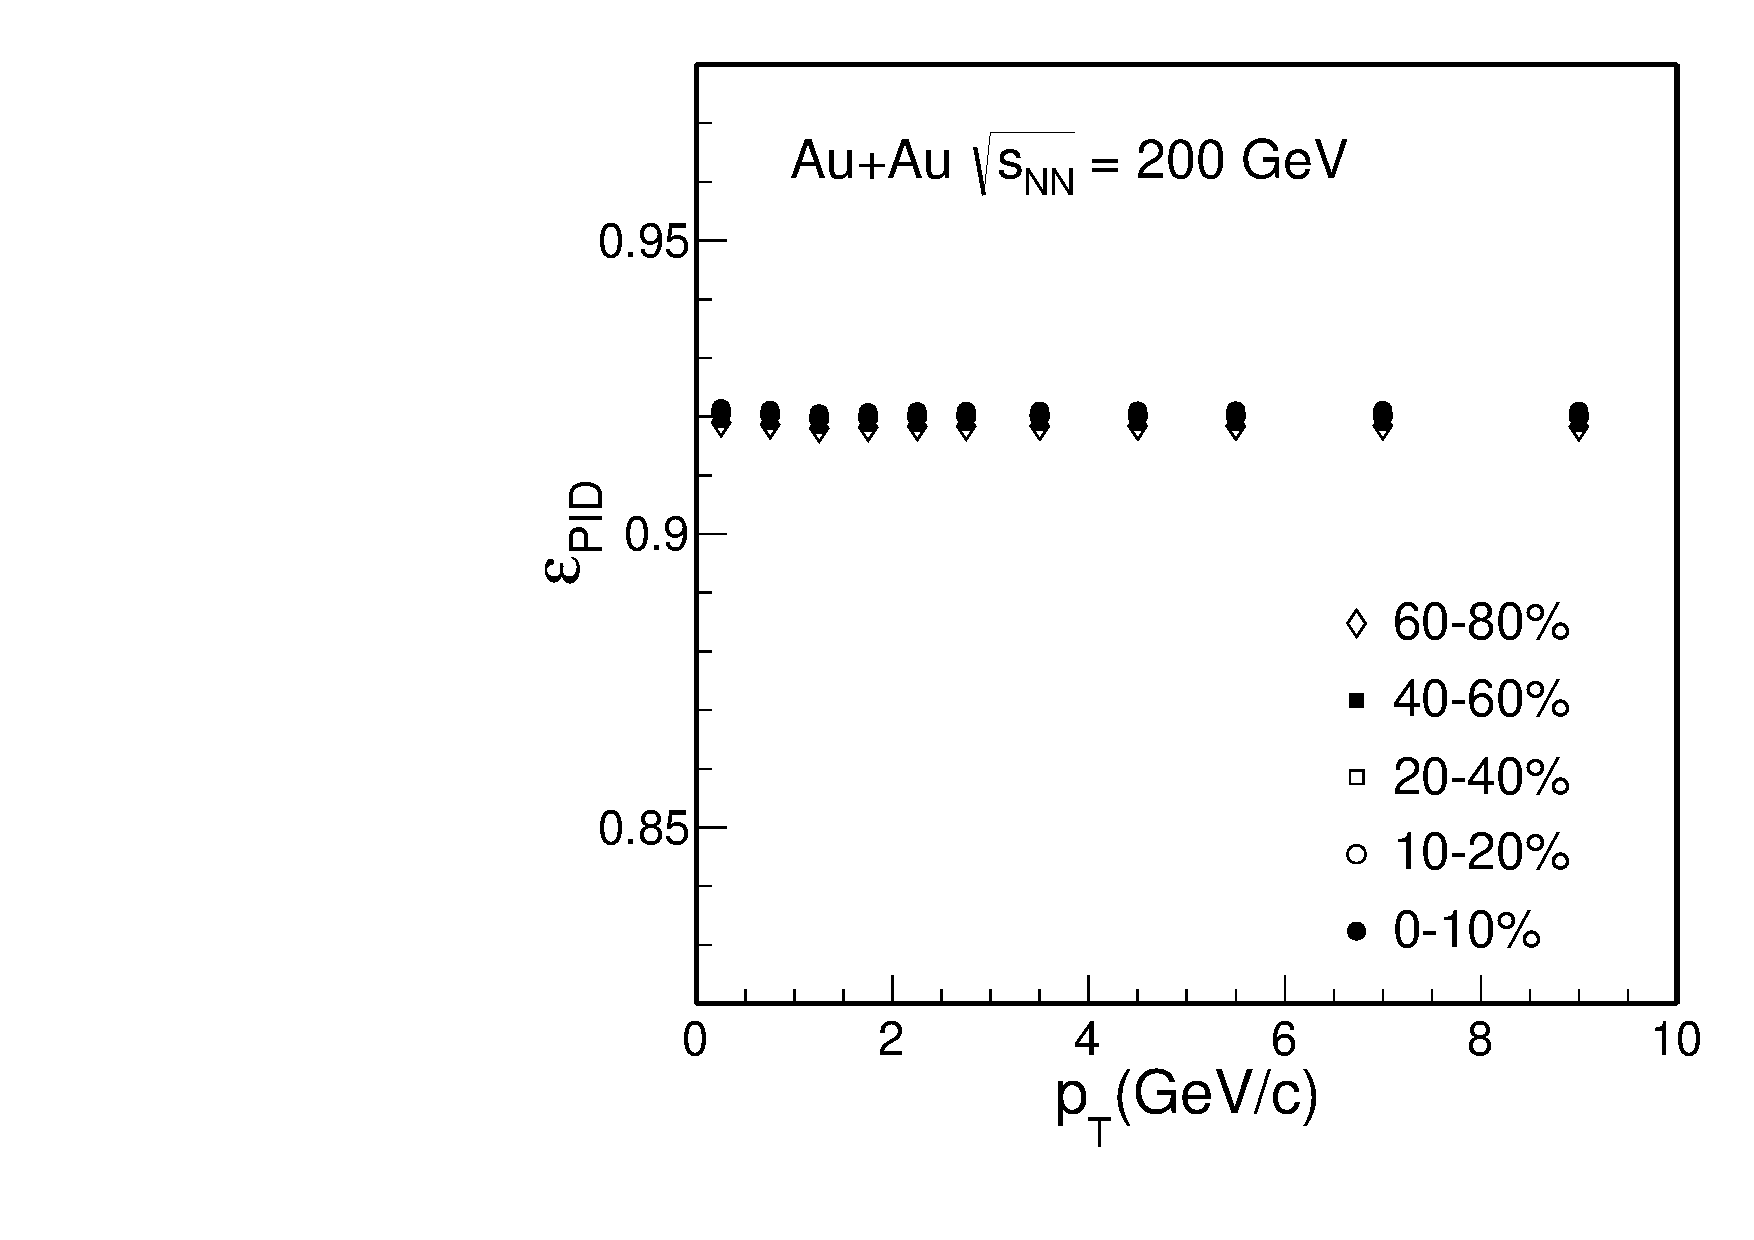
\includegraphics[width=0.43\textwidth]{fig/Datad0Eff_pid_10.pdf}
\caption{Particle identification efficiency ($\varepsilon_{\rm PID}$) of $D^0$ mesons in different centrality classes in Au + Au collisions at $\sqrt{s_{_{\rm NN}}}$ = 200\,GeV.}
\label{fig:Datad0Eff_pid} 
\end{figure}

\begin{figure}
\centering
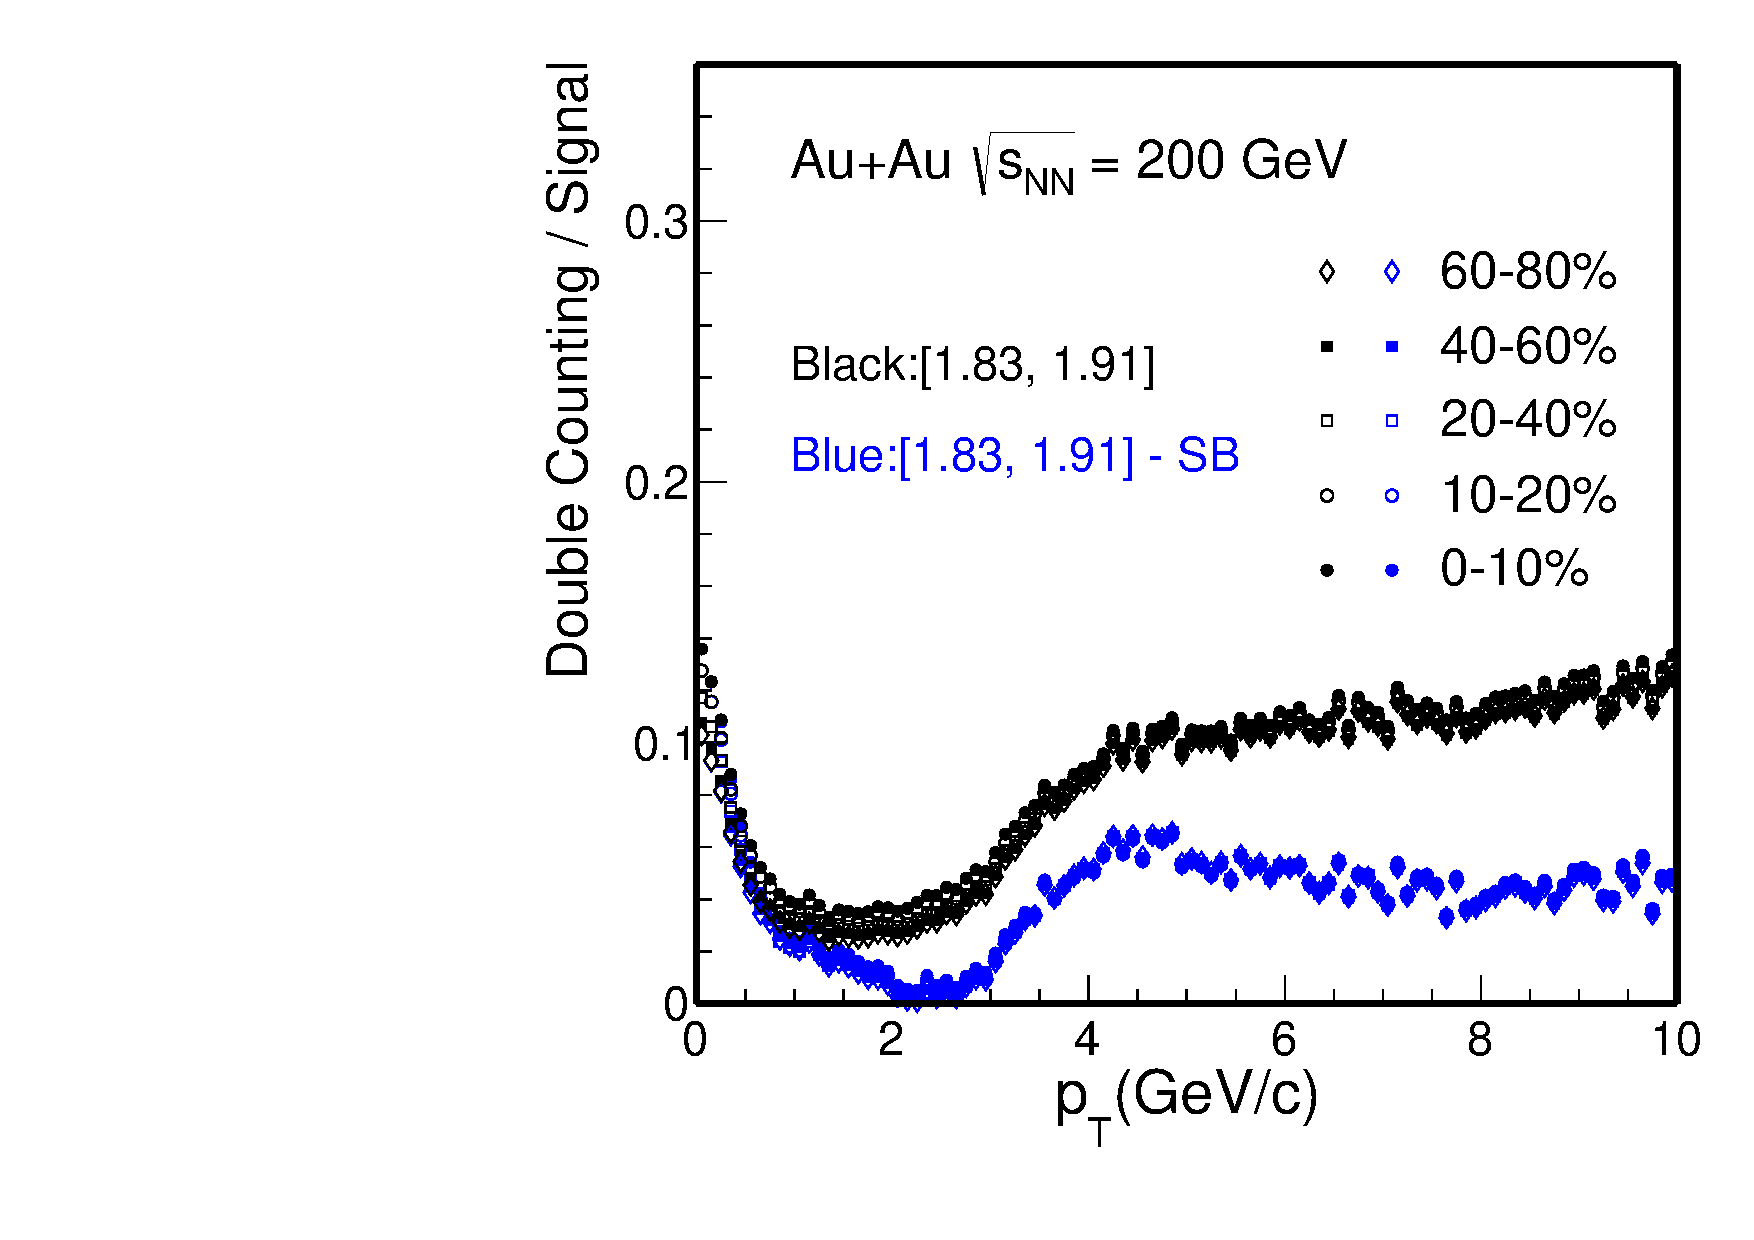
\includegraphics[width=0.43\textwidth]{fig/Double_counting.pdf}
\caption{$D^{0}$ yield double counting fraction due to doubly mis-PID in different centrality classes in Au + Au collisions at $\sqrt{s_{_{\rm NN}}}$ = 200\,GeV. The black markers depict an estimation taking the total double counting yield in the $D^0$ mass window while the blue markers depict an estimation with an additional side-band (SB) subtraction.}
\label{fig:Datad0Eff_doublecounting} 
\end{figure}

The $D^0$ daughter particle identification (PID) cut efficiency includes contributions from the $dE/dx$ selection cut efficiency as well as the TOF matching and $1/\beta$ cut efficiency. To best estimate the selection cut efficiency, we select the pure kaon and pion samples from V0 decay following the same procedure as in~\cite{Shao:2005iu,Xu:2008th}. The $dE/dx$ cut efficiencies for pion and kaon daughter tracks are calculated respectively. The TOF $1/\beta$ cut efficiency is determined by studying the $1/\beta$ distributions for kaons and pions in the clean separation region, namely $p_{\rm T}<$ 1.5\,GeV/$c$. There is a mild dependence for the offset and width of $\Delta 1/\beta$ distributions vs. particle momentum and our selection cuts are generally wide enough to capture nearly all tracks once they have valid $\beta$ measurements. The total PID efficiency of $D^0$ mesons is calculated by folding the individual track TPC and TOF PID efficiencies following the same hybrid PID algorithm as implemented in the data analysis. Fig.~\ref{fig:Datad0Eff_pid} shows the total PID efficiencies for $D^0$ reconstruction in various centrality bins. The total PID efficiency is generally high and there is nearly no centrality dependence.

When the $D^0$ daughter kaon track is mis-identified as a pion track and the other daughter pion track is mis-identified as a kaon track, the pair invariant mass distribution will have a bump structure around the real $D^0$ signal peak, but the distribution is much broader in a wide mass region due to the mis-assigned daughter particle masses. Based on the PID  performance study described above, we estimate the single kaon and pion candidate track purities. After folding the realistic particle momentum resolution, we calculate the reconstructed $D^0$ yield from doubly mis-identified pairs (double counting) underneath the real $D^0$ signal and the double counting fraction is shown in Fig.~\ref{fig:Datad0Eff_doublecounting}. The black markers show the fraction by taking all doubly mis-identified pairs in the $D^0$ mass window while the blue markers depict that with an additional side-band (SB) subtraction. The latter is used as a correction factor to the central values of reported $D^0$ yields while the difference between the black and blue symbols are considered as the systematic uncertainty in this source. The double counting fraction is below 10\% in all $p_{\rm T}$ bins, and also there is little centrality dependence.

\begin{figure}
\centering
% 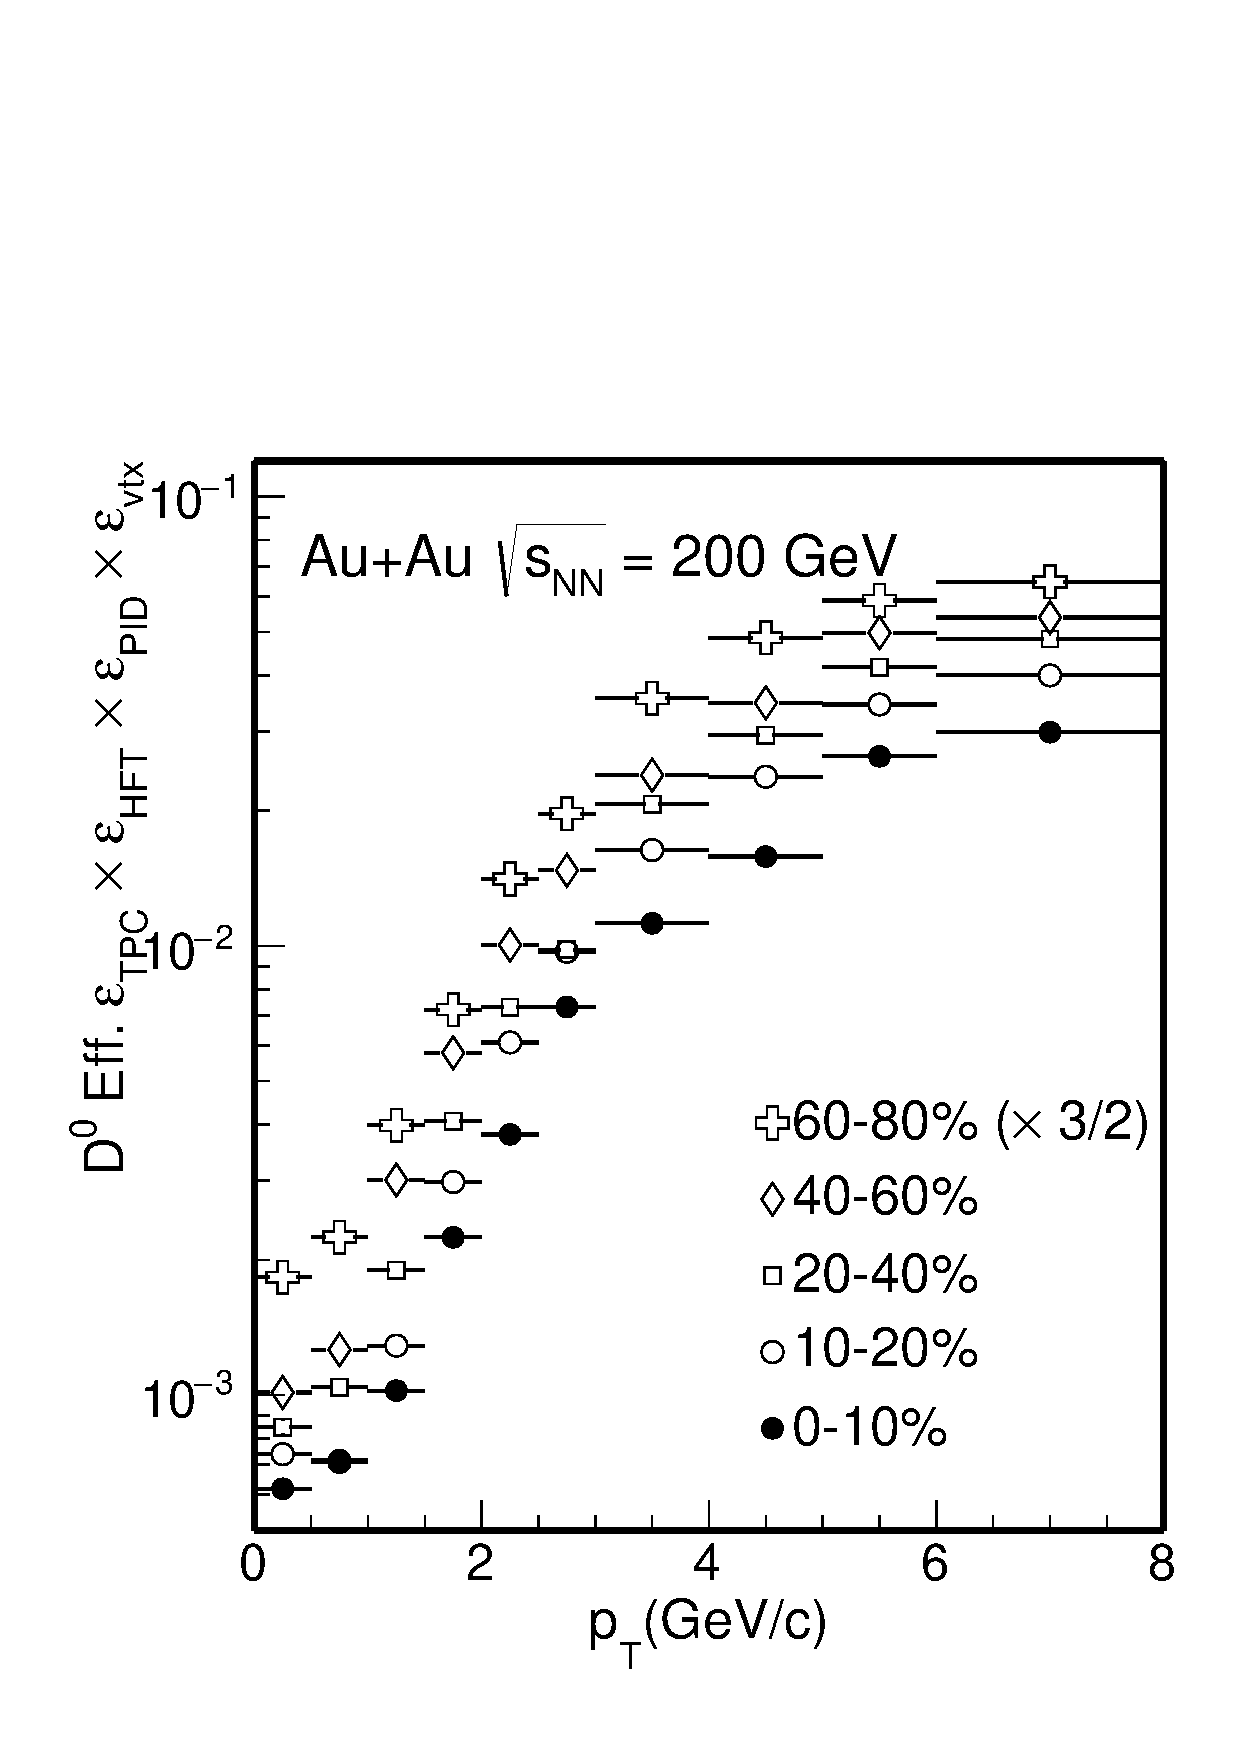
\includegraphics[width=0.4\textwidth]{fig/Datad0Eff.pdf}
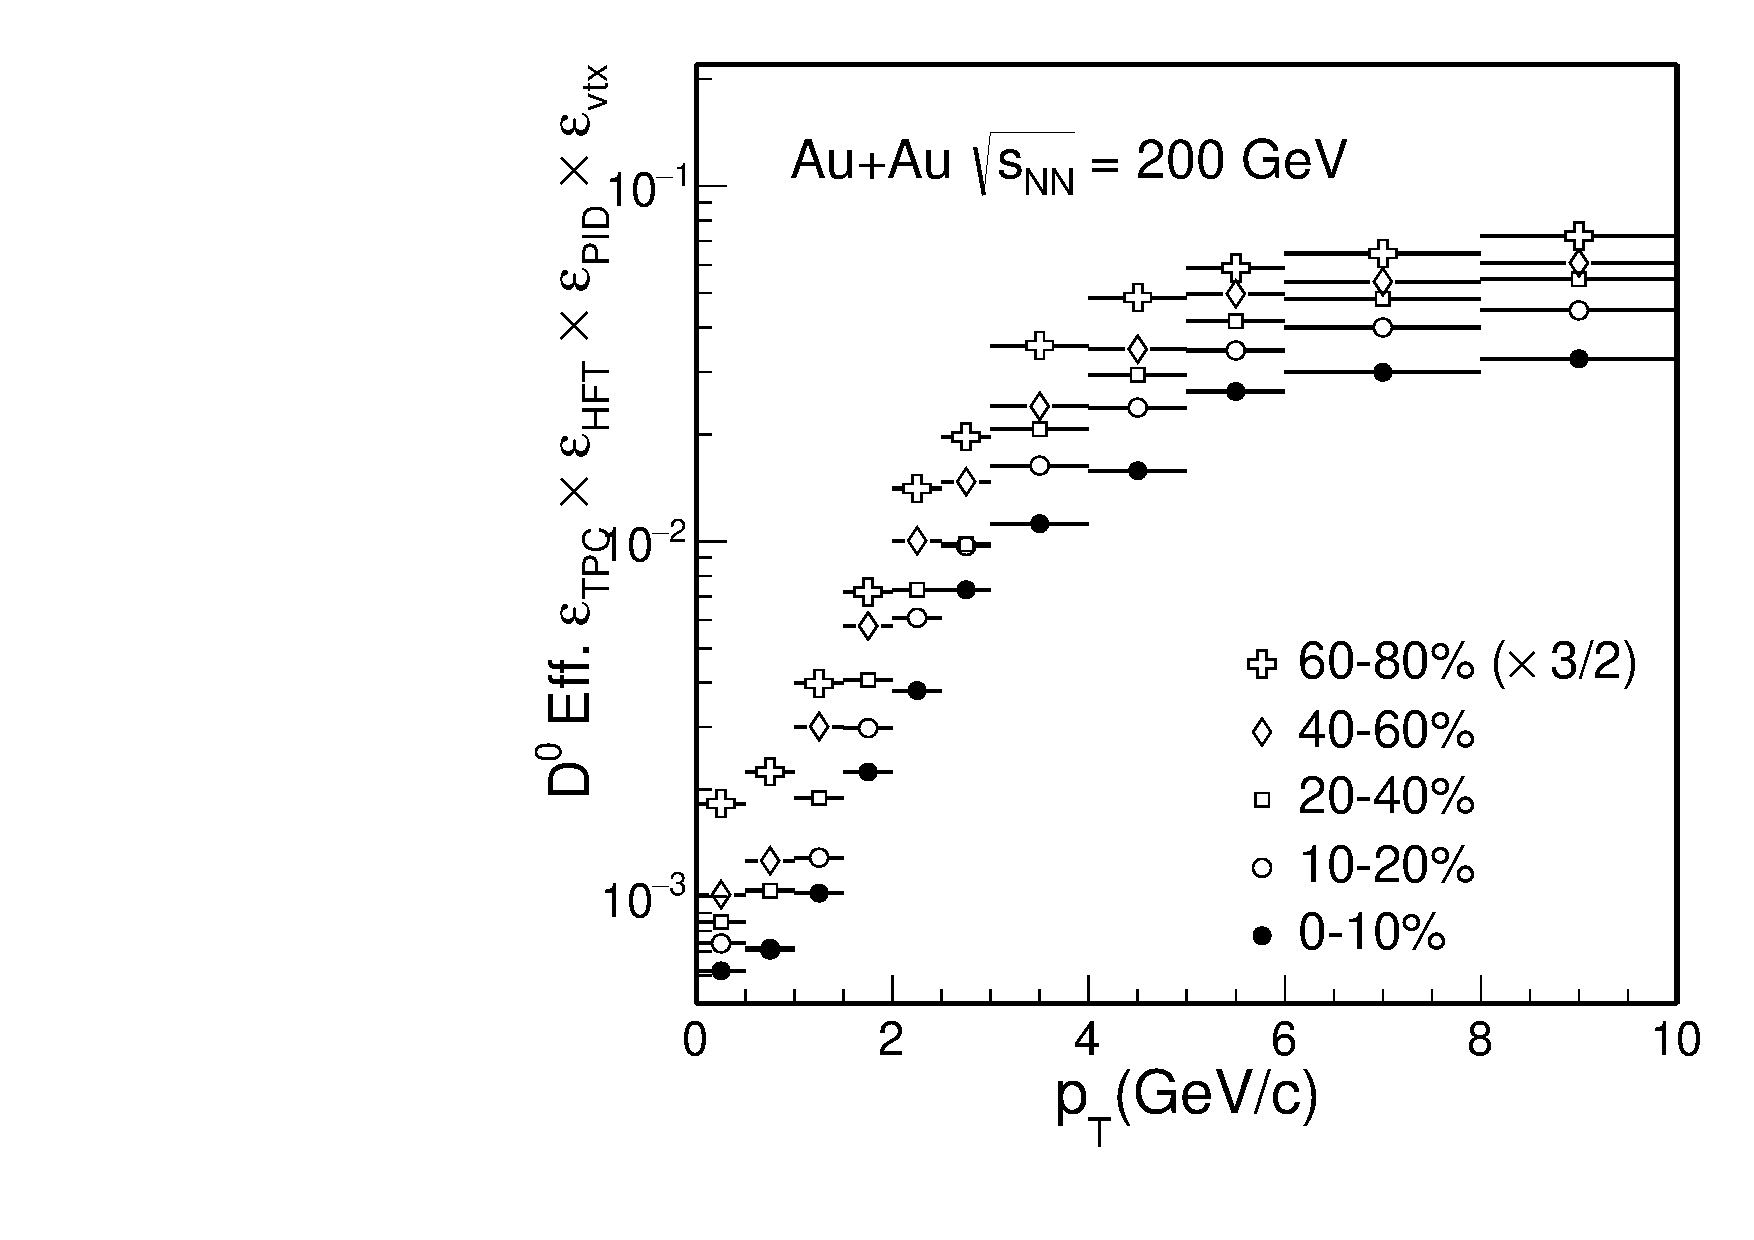
\includegraphics[width=0.43\textwidth]{fig/Datad0Eff_10.pdf}
\caption{The total $D^{0}$ reconstruction efficiency from different centrality classes in Au + Au collisions at $\sqrt{s_{_{\rm NN}}}$ = 200\,GeV.}
\label{fig:Datad0Eff} 
\end{figure}

\section{\label{sec:systematic}Systematic Uncertainties}

The systematic uncertainty on the final measured $D^0$ $p_{\rm T}$ spectra can be categorized into the uncertainty of the raw $D^0$ yield extraction and the uncertainty of efficiencies and corrections.

The uncertainty of the raw yield extraction is estimated by a) the difference in the $D^0$ yield obtained with the fit and bin counting methods and b) varying invariant mass ranges for fit and for side bands and c) varying background estimation from mixed-event and like-sign methods. The maximum difference between these scenarios is then converted to the standard deviation and added to the systematic uncertainties. It is the smallest in the mid-$p_{\rm T}$ bins due to the best signal significance and grows at both low and high $p_{\rm T}$. The double counting contribution in the $D^0$ raw yield  due to mis-PID is included as another contribution to the systematic uncertainty for the $D^0$ raw yield extraction as described in Sec.~\ref{sec:correction:PID}.

The uncertainty of the TPC acceptance and efficiency correction $\varepsilon_{\rm TPC}$ is estimated via the standard procedure in STAR by comparing the TPC track distributions between real data and the embedding data. It is estimated to be $\sim 3-6\%$ for 0-10\% collisions and $\sim 3-7\%$ for 60-80\% collisions, and they are largely correlated for different centralities and $p_{\rm T}$ regions. 

The uncertainty of the PID efficiency correction is estimated by varying the PID selection cuts and convert to the final corrected $D^0$ yield. 

% The uncertainty of the PID efficiency correction is estimated by varying the PID selection cuts and compare the difference in the final corrected $D^0$ yield. In addition, for the TOF PID, we also consider the finite TOF acceptance and matching efficiency uncertainty.

% {\color{red}{Guannan: please confirm the numbers below}}
To estimate the uncertainty of the HFT tracking and topological cut efficiency correction $\varepsilon_{\rm HFT}$, we employ the following procedures: a) We vary the topological variable cuts so the $D^0$ $\varepsilon_{\rm HFT}$ is changed to 50\% and 150\% of the nominal (default) efficiency and compare the efficiency corrected final $D^0$ yields. The maximum difference between the two scenarios is then added to the systematic uncertainties. b) We also vary the daughter $p_{\rm T}$ low threshold cut between 0.3 to 0.6 GeV/$c$ and the maximum difference in the final corrected $D^0$ yield is also included in the systematic uncertainties. c) We add the systematic uncertainty due to limitation of the data-driven simulation approach, $\sim$5\% and the impact of the secondary particles $\sim$2\% to the total $\varepsilon_{\rm HFT}$ systematic uncertainty.% for the 0-20\% central collisions.

With the corrected $D^0$ transverse momentum spectra, nuclear modification factor $R_{\rm CP}$ is calculated as the ratio of $N_{\rm bin}$ normalized yields between central and peripheral collisions, as shown in the following formula. 

\[
R_{\rm CP} = \frac{d^2N/dp_{\rm T}dy/N_{\rm bin}|_{\rm cen}}{d^2N/dp_{\rm T}dy/N_{\rm bin}|_{\rm peri}}
\]

The systematic uncertainties in raw signal extraction in central and peripheral collisions are propagated as they are uncorrelated, while systematic uncertainties in many other sources are correlated or partially correlated in contributing to the measured $D^0$ yields. To best consider these correlations, we vary different variables simultaneously in central and peripheral collisions, and the difference in the final extracted $R_{\rm CP}$ value is then directly counted as systematic uncertainties in the measured $R_{\rm CP}$.

Nuclear modification factor $R_{\rm AA}$ is calculated as the ratio of $N_{\rm bin}$ normalized yields between Au + Au and p + p collisions. The baseline choose and uncertainties sources for p + p collisions are the same as the publication~\cite{Star_D_RAA_corr}. The uncertainties from the p + p reference dominates this systematic uncertainty, which include the 1 $\sigma$ uncertainty from the Levy fit and the difference between Levy and power-law function fits for extrapolation to low and high $p_T$, expressed as 1 standard deviation.

With the corrected $D^0$ and $\overline{D}^{0}$ transverse momentum spectra, $\overline{D}^{0}/D^0$ ratio is calculated as a function of the transverse momentum. The systematic uncertainties in raw signal extraction for $\overline{D}^{0}$ and $D^0$ are propagated as they are uncorrelated, while systematic uncertainties in many other sources are correlated or partially correlated in contributing to the measured $\overline{D}^{0}/D^0$ ratio. As in the $R_{\rm CP}$ systematic uncertainty estimation, we vary different variables simultaneously for $D^0$ and $\overline{D}^{0}$, and the difference in the final extracted $\overline{D}^{0}/D^0$ value is then directly counted as systematic uncertainties in the measured $\overline{D}^{0}/D^0$.

\begin{table*}
\centering{
\caption{Summary of systematic uncertainties, in percentage, on the $D^0$ invariant yield in 0-10\% and 60-80\% collisions and $R_{\rm CP}$(0-10\%/60-80\%).}
\begin{tabular}{c|cc|c|c} \hline \hline
Source & \multicolumn{3}{c|}{Systematic Uncertainty} & Correlation in $p_{\rm T}$\\ \cline{2-4}
       & \hspace{1cm}0--10\%\hspace{1cm} & \hspace{1cm}60--80\%\hspace{1cm} & \hspace{1cm}$R_{\rm CP}$(0--10\%/60--80\%)\hspace{1cm} &  \\ \hline \hline
Signal extra. & 1-6  & 1-12  & 2-13\ & uncorr. \\ \hline
Double mis-PID & 1-7  & 1-7  & negligible & uncorr. \\ \hline \hline
$\varepsilon_{\rm TPC}$ & 3-6 & 3-7 & 3-7 & largely corr. \\ \hline
$\varepsilon_{\rm HFT}$ & 3-15 & 3-20 & 3-20 & largely corr. \\ \hline
$\varepsilon_{\rm PID}$ & 3 & 3 & negligible & largely corr. \\ \hline
$\varepsilon_{\rm vtx}$ & 5 & 9-18 & 10-18 & largely corr. \\ \hline
BR. & \multicolumn{2}{c|}{0.5} & 0 & global \\ \hline \hline
$N_{\rm bin}$ & 2.8 & 42 & 42 & global \\ \hline \hline
\end{tabular}
}
\label{table:syserror}
\end{table*}


Table~\ref{table:syserror} summarizes the systematic uncertainty sources and their contributions, in percentage, on the $D^0$ invariant yield in 0-10\% and 60-80\% collisions and $R_{\rm CP}$(0-10\%/60-80\%). In the last column we also comment on the correlation in $p_{\rm T}$ for each individual source. Later when reporting $p_{\rm T}$ integrated yields or $R_{\rm CP}$, systematic uncertainties are calculated under the following considerations: a) for $p_{\rm T}$ uncorrelated sources, we take the quadratic sum of various $p_{\rm T}$ bins; b) for sources that are largely correlated in $p_{\rm T}$, we take the arithmetic sum as an conservative estimate.

%The systematic uncertainties are studied for the spectra and $R_{\rm CP}$ analysis. Several sources are contributed to the uncertainties. Such as the TPC tracking, the raw yield extraction, the daughter $p_T$ cut scan, the topological cuts scan, the double counting and the vertex resolution contribution and so on. %The TPC uncertainties are studied by comparison of the tracking performance from real data and the MC simulation. A few different methods are used to extract the raw $D^0$ signal counts, for example using the like-sign method or mixed-event technique to subtract the combinatorial background, or using the binning counting method instead of directly fitting method to extract the yield. Several different daughter $p_T$ cuts are applied on the $D^0$ reconstruction and corrected for the efficiency. We also varied the topological variables for the reconstruction with a quite different reconstruction efficiency. The mis-identification from the daughter particles are studied. The vertex resolution is also discussed in the previous section.

% Chapter four
\
\section{\label{result}Results and Discussion}

\subsection{\label{result:pt}$p_{\rm T}$ Spectra and Integrated Yields}
Figure~\ref{fig:D0_spectra} shows the efficiency-corrected $D^0$ invariant yield at mid-rapidity ($|y|<1$) vs. $p_{\rm T}$ in 0--10\%, 10--20\%, 20--40\%, 40--60\%, 60--80\% and 0--80\% Au + Au collisions at $\sqrt{s_{_{\rm NN}}}$ = 200\,GeV. $D^0$ spectra in some centrality bins are arbitrarily scaled with factors indicated on the plot for clarity. Dashed and solid lines depict fits to the spectra with the Levy function

\begin{widetext}
\[
\frac{d^2N}{2\pi p_{\rm T}dp_{\rm T}dy} = \frac{1}{2\pi}\frac{dN}{dy}\frac{(n-1)(n-2)}{nT(nT+m_0(n-2))}\bigg(1+\frac{\sqrt{p_{\rm T}^2+m_0^2}-m_0}{nT}\bigg)^{-n}
\]
\end{widetext}

where $m_0$ is the $D^0$ mass and $\frac{dN}{dy}$, $T$ and $n$ are free parameters. The Levy function fit describes the $D^0$ spectra nicely in all centrality bins up to 8\,GeV/$c$.

\begin{figure}
\centering
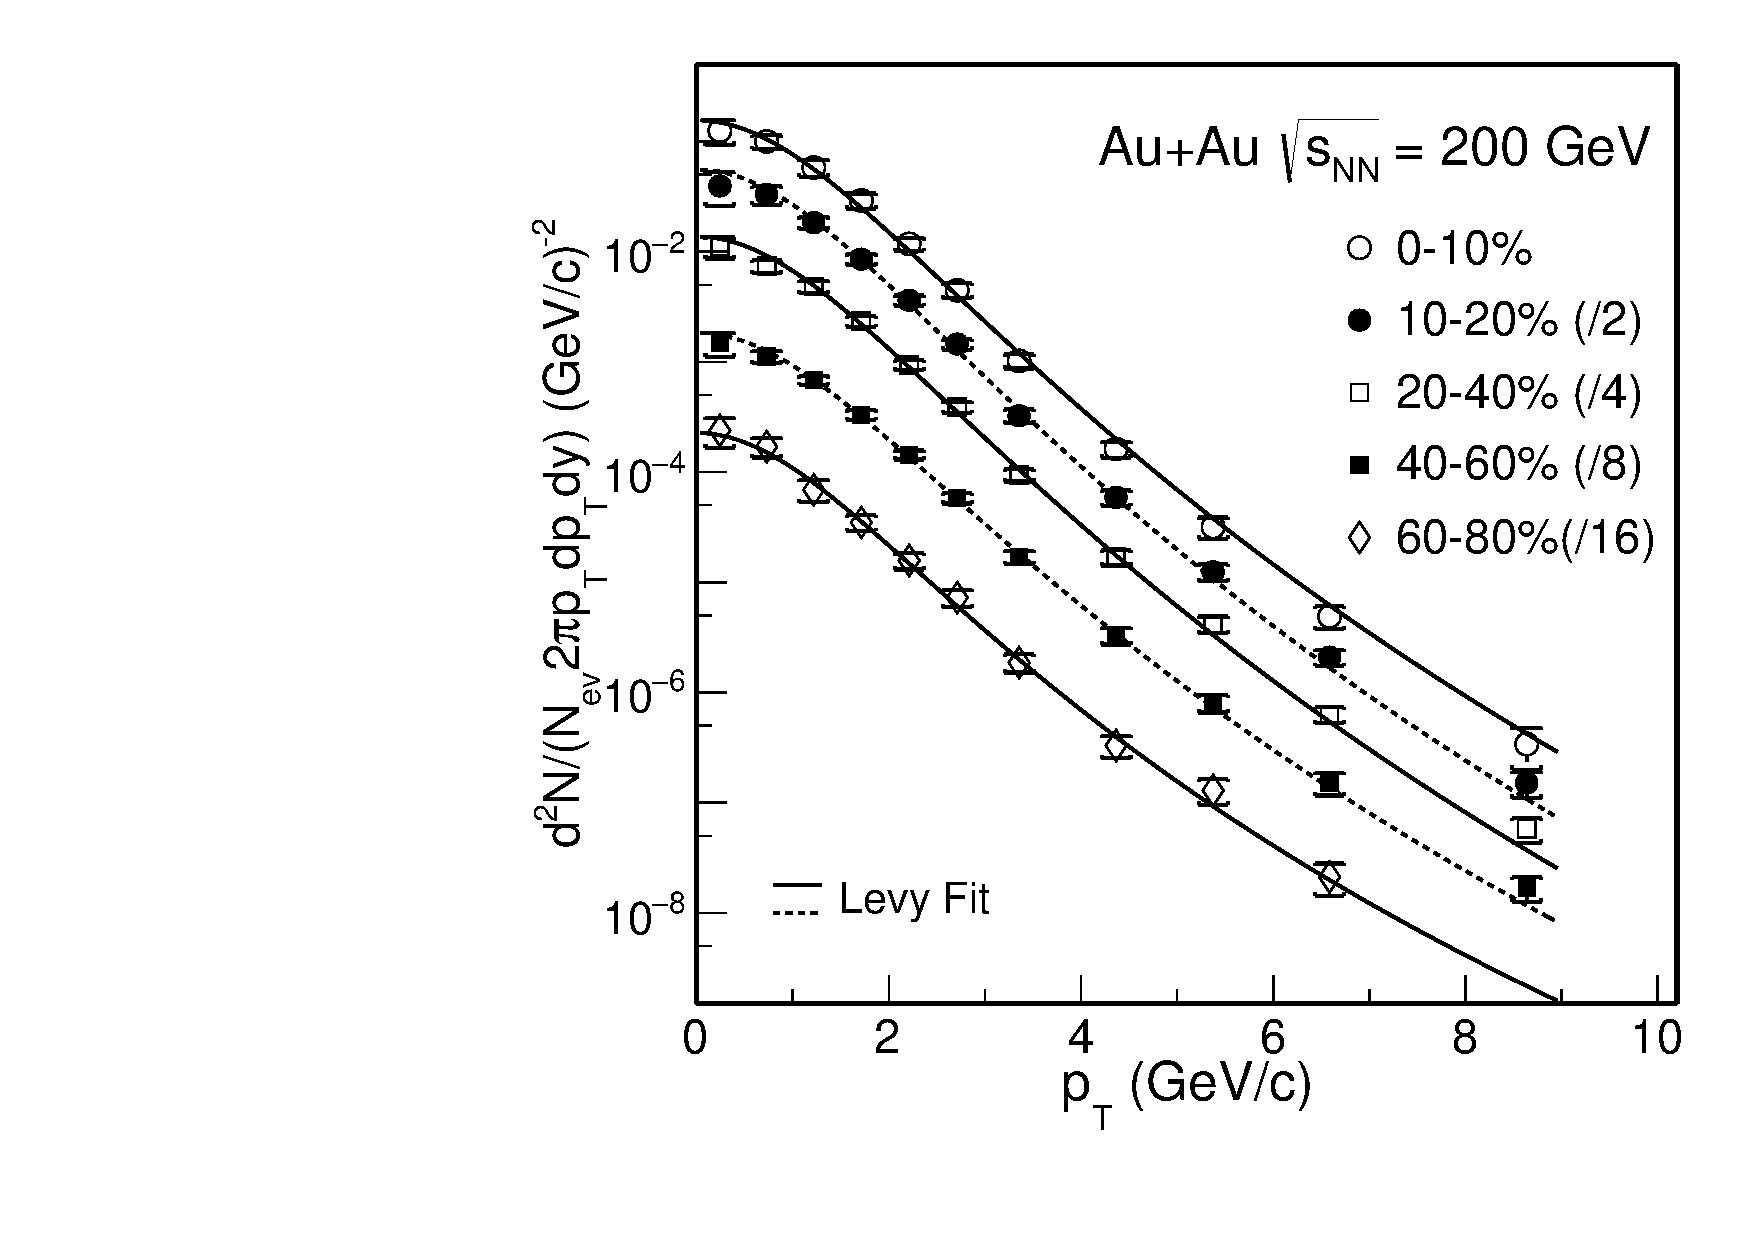
\includegraphics[width=0.43\textwidth]{fig/D0_spectra.pdf}
\caption{$D^{0}$ invariant yield at mid-rapidity ($|y|<1$) vs. transverse momentum for different centrality classes in Au + Au collisions at $\sqrt{s_{_{\rm NN}}}$ = 200\,GeV. Error bars (not visible for many data points) indicate statistical uncertainties and brackets depict systematical uncertainties. Global systematic uncertainties in $B.R.$ are not plotted. Solid and dashed lines depict Levy function fits.}
\label{fig:D0_spectra} 
\end{figure}

We compare our new measurements with previous measurements using the STAR TPC only. The previous measurements are recently corrected after fixing errors in the TOF PID efficiency calculation~\cite{Star_D_RAA,Star_D_RAA_corr}. Fig.~\ref{fig:D0_compareSpectra_run10} shows the $p_{\rm T}$ spectra comparison in 0--10\%, 10-40\% and 40--80\% centrality bins in panel (a) and the ratios to the levy fit functions are shown in panel (b), (c), and (d). The new measurement with the HFT detector shows a nice agreement with the measurement without the HFT, but with significantly improved precision.

\begin{figure}
\centering
\includegraphics[width=0.43\textwidth]{fig/D0_compareSpectra_run10.eps}
\caption{Measured $D^{0}$ spectra from this analysis compared with the previous 2010/11 measurements for different centrality classes in Au + Au collisions at $\sqrt{s_{_{\rm NN}}}$ = 200\,GeV.}
\label{fig:D0_compareSpectra_run10} 
\end{figure}


The measured $D^0$ spectra cover a wide $p_{\rm T}$ region which allows us to extract the $p_{\rm T}$ integrated total $D^0$ yield at mid-rapidity with good precision. Fig.~\ref{fig:Xsection_D0} shows the $p_{\rm T}$ integrated cross section $d\sigma/dy|_{y=0}$ for $D^0$ production per nucleon-nucleon collision from different centrality bins for the full $p_{\rm T}$ range shown in the top panel and for $p_{\rm T}>$ 4\,GeV/$c$ shown in the bottom panel. The result from previous $p+p$ measurement is also shown in the top panel.

The total $D^0$ cross section per nucleon-nucleon collision at mid-rapidity $d\sigma/dy|_{y=0}$ shows approximately a flat distribution as a function of centrality, even though the systematic uncertainty in the 60--80\% centrality bin is a bit large. The values in mid-central to central Au+Au collisions are smaller than that in $p+p$ collisions with $\sim$ 1.5$\sigma$ effect considering the large uncertainties from the $p+p$ measurements. The total charm quark yield in heavy-ion collisions is expected to follow the number-of-binary-collision scaling since charm quarks are believed to be predominately created at the initial hard scattering before the formation of the QGP at RHIC energies, while the cold nuclear effect could also play an important role. In addition, coalescence hadronization mechanism has been suggested to potentially modify the charm quark distribution in various charm hadron states which may lead to the reduction in the observed $D^0$ yields in Au+Au collisions. For instance, coalescence hadronization can lead to an enhancement in the charmed baryon $\Lambda_{c}^+$ yield relative to $D^0$ yield~\cite{Oh2009}, and together with the strangeness enhancement in the hot QCD medium, can also lead to an enhancement in the charmed strangeness meson $D_{s}^+$ yield relative to $D^0$~\cite{He2013}. Therefore, determination of the total charm quark yield in heavy-ion collisions will require measurements of other charm hadron states over a broad momentum range.

\begin{figure}
\centering
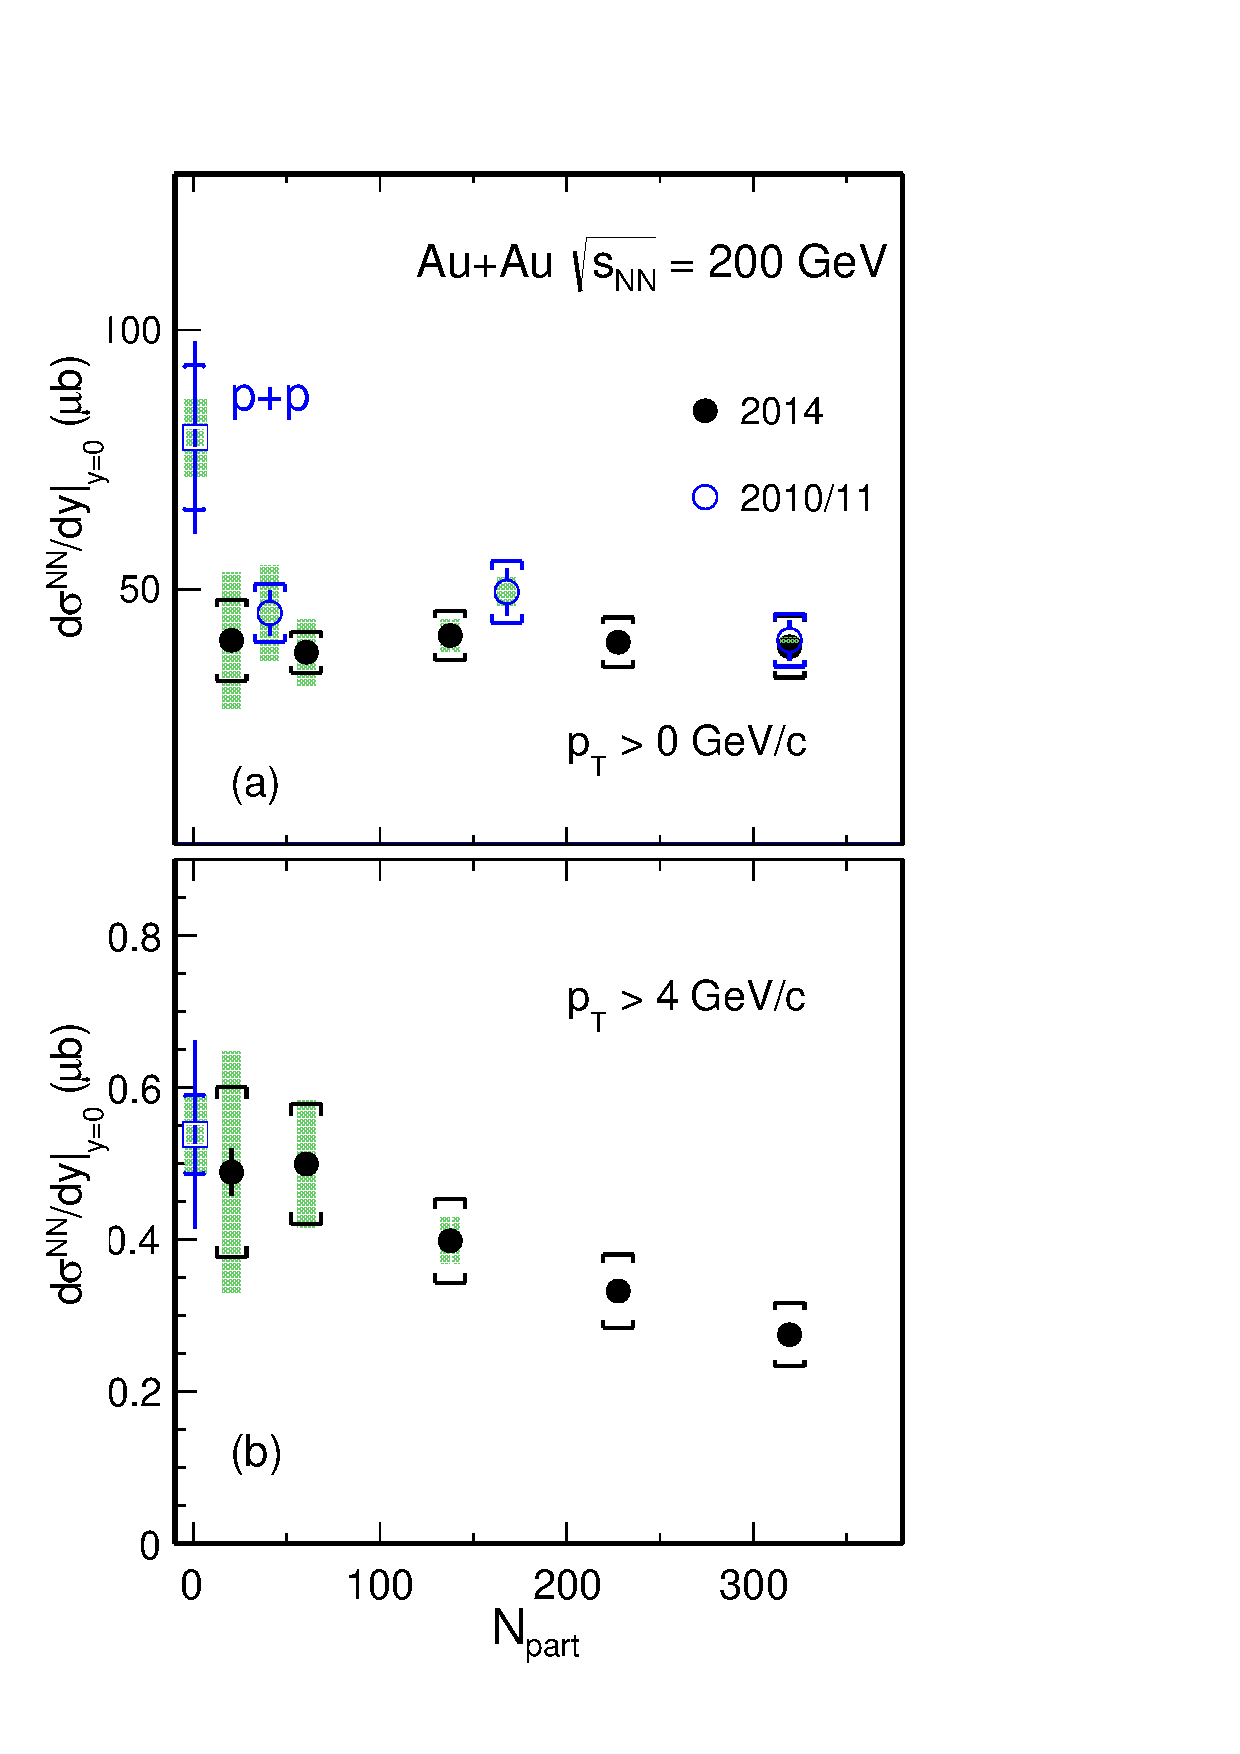
\includegraphics[width=0.43\textwidth]{fig/Xsection_D0.pdf}
\caption{Integrated $D^{0}$ cross section at mid-rapidity per nucleon-nucleon collision at mid-rapidity for $p_{\rm T}>0$ and $p_{\rm T}>4$\,GeV/$c$ as a function of centrality $N_{\rm part}$. The statistical and systematic uncertainties are shown as error bars and brackets on the data points. The green boxes on the data points depict the overall normalization uncertainties in p + p and Au + Au data respectively.}
\label{fig:Xsection_D0} 
\end{figure}

\subsection{\label{result:collectivity}Collectivity}

\subsubsection{\label{result:collectivity:mT}$m_{\rm T}$ Spectra}

\begin{figure}
\centering
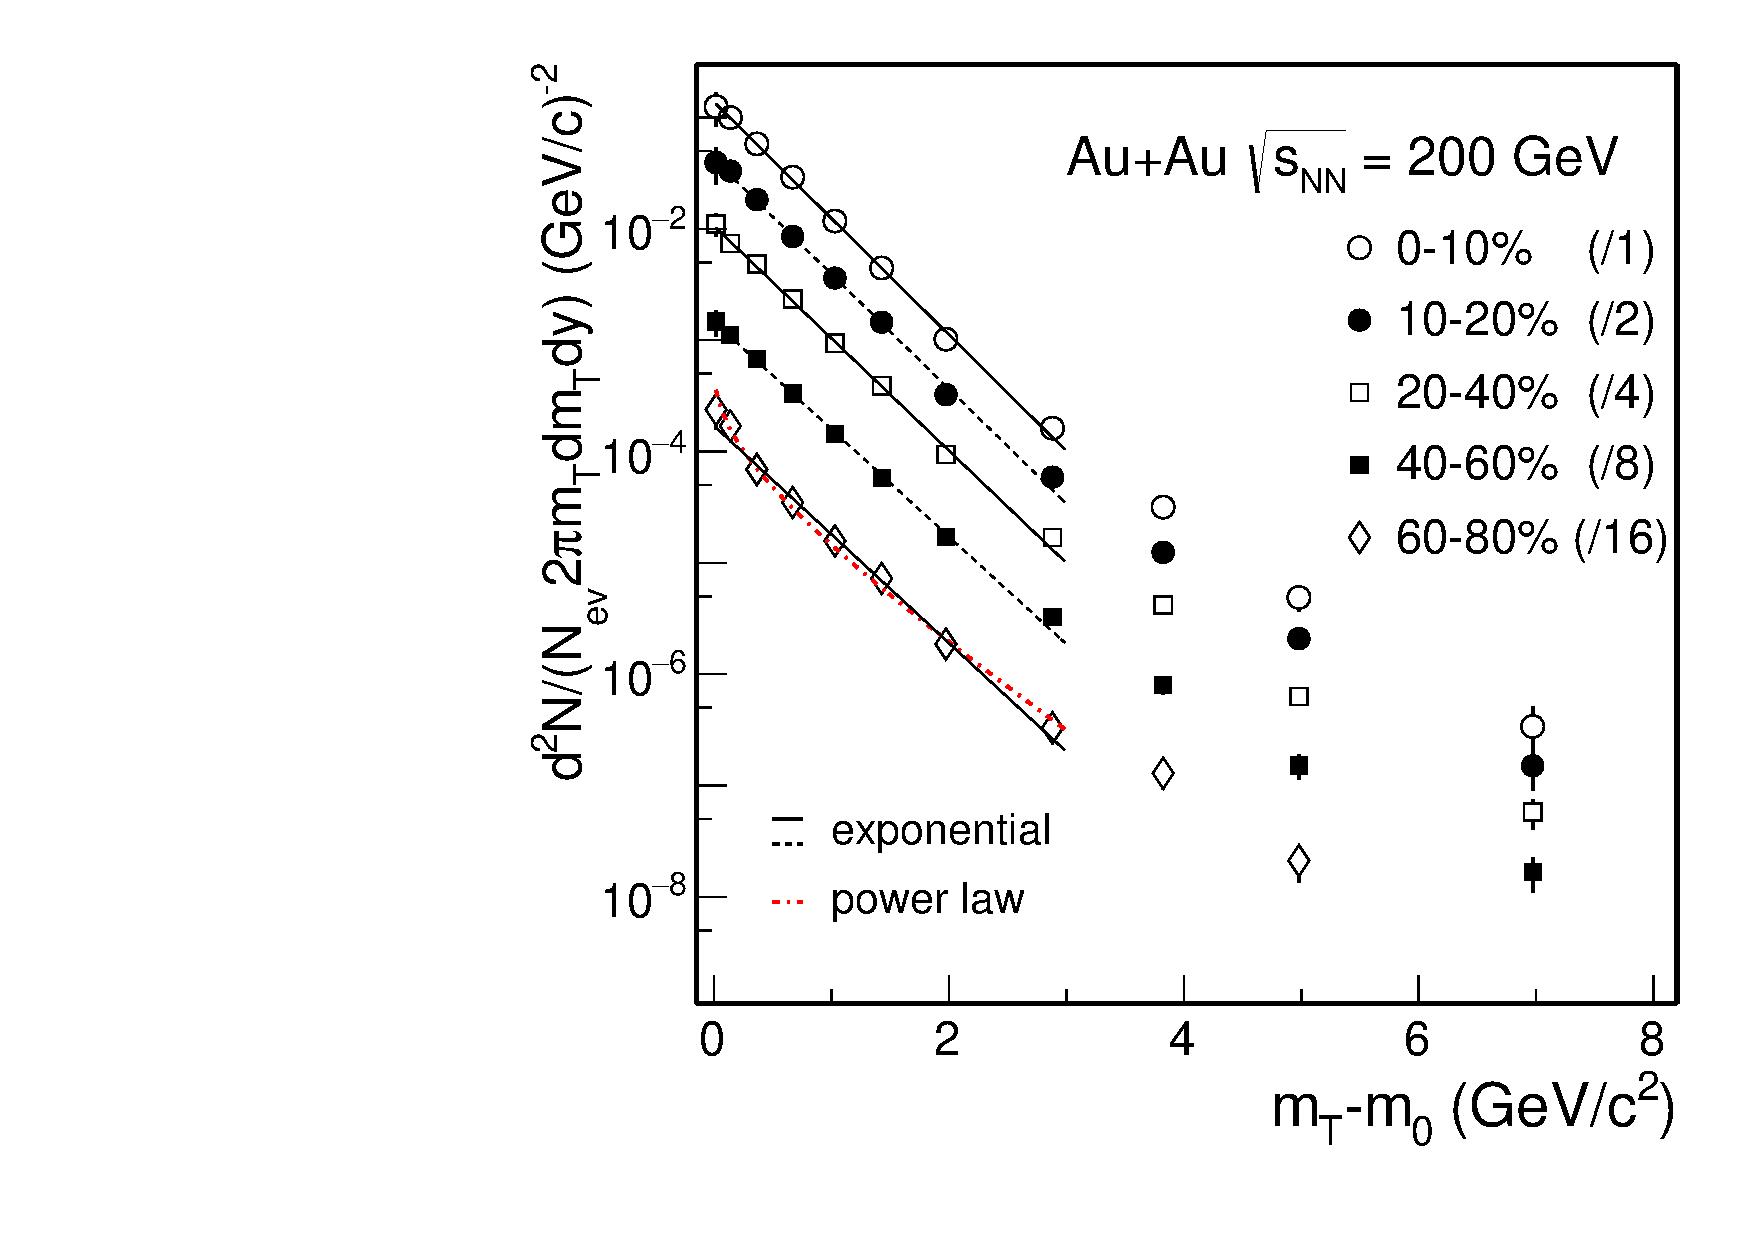
\includegraphics[width=0.43\textwidth]{fig/mTFit_D0.pdf}
\caption{$D^{0}$ invariant yield at mid-rapidity ($|y|<1$) vs. transverse kinetic energy ($m_{T}$ - $m_{0}$) for different centrality classes in Au + Au collisions at $\sqrt{s_{_{\rm NN}}}$ = 200\,GeV. Error bars (not visible for many data points) indicate statistical uncertainties and brackets depict systematical uncertainties. Global systematic uncertainties in $B.R.$ are not plotted. Solid and dashed black lines depict exponential function fits and the dot-dashed line depict a power-law function fit to the spectrum in 60--80\% centrality bin.}
\label{fig:mTFit_D0} 
\end{figure}

Transverse mass spectra can be used to study the collectivity of produced hadrons in heavy-ion collisions. Fig.~\ref{fig:mTFit_D0} shows the $D^{0}$ invariant yield at mid-rapidity ($|y|<1$) vs. transverse kinetic energy ($m_{\rm T}$ - $m_{0}$) for different centrality classes in Au + Au collisions at $\sqrt{s_{_{\rm NN}}}$ = 200\,GeV, where $m_{\rm T} = \sqrt{p_{\rm T}^2+m_0^2}$ and $m_0$ is the $D^0$ meson mass. Solid and dashed black lines depict thermal model inspired exponential function fits to data in various centrality bins up to $m_{\rm T} - m_{0}$ $<3$\,GeV/$c^2$ using the fit function shown below
\[
\frac{d^2N}{2\pi m_{\rm T}dm_{\rm T}dy} = \frac{dN/dy}{2\pi T_{\rm eff}(m_0+T_{\rm eff})}e^{-(m_{\rm T}-m_0)/T_{\rm eff}}
\]
Such a method has been often used to analyze the particle spectra and to understand kinetic freezeout properties for the data in heavy ion collisions~\cite{Kaneta:1999lnf,StarWhitePaper}.


A power-law function (shown below) is also used to fit the spectrum in 60--80\% centrality bin. 

%\begin{widetext}
\[
\frac{d^2N}{2\pi p_{\rm T}dp_{\rm T}dy} = \frac{dN}{dy}\frac{4(n-1)(n-2)}{2\pi (n-3)^2\langle p_{\rm T} \rangle ^2}\bigg(1+\frac{2p_{\rm T}}{\langle p_{\rm T} \rangle (n-3)}\bigg)^{-n}
\]
%\end{widetext}

where $dN/dy$, $\langle p_{\rm T}\rangle$, and $n$ are three free parameters.

The power-law function fit shows a good description to the 60--80\% centrality data indicating the $D^0$ meson production in this peripheral bin is close to the expected feature of the perturbative QCD. The $D^0$ meson spectra in more central collisions can be well described by the expotential function fit at $m_{\rm T}$ - $m_{0}$ $<3$\,GeV/$c^2$ suggesting the $D^0$ mesons have gained collectivity in the medium evolution in these collisions.


% Figure~\ref{fig:Teff_D0} shows the $m_{\rm T}$ spectra slope parameter $T_{\rm eff}$ (obtained from the expontential fit described above) vs. collision centrality. Statistical and point-to-point systematic uncertainties, but no global systematic uncertainties, are added quadratically when performing the expontial fit. Therefore uncertainties shown in this plot are the total uncertainties on this fit parameter. The obtained $T_{\rm eff}$ parameter increases from peripheral to central collisions, suggesting more collectivity that $D^0$ mesons gain in more central collisions. 

% \begin{figure}
% \centering
% 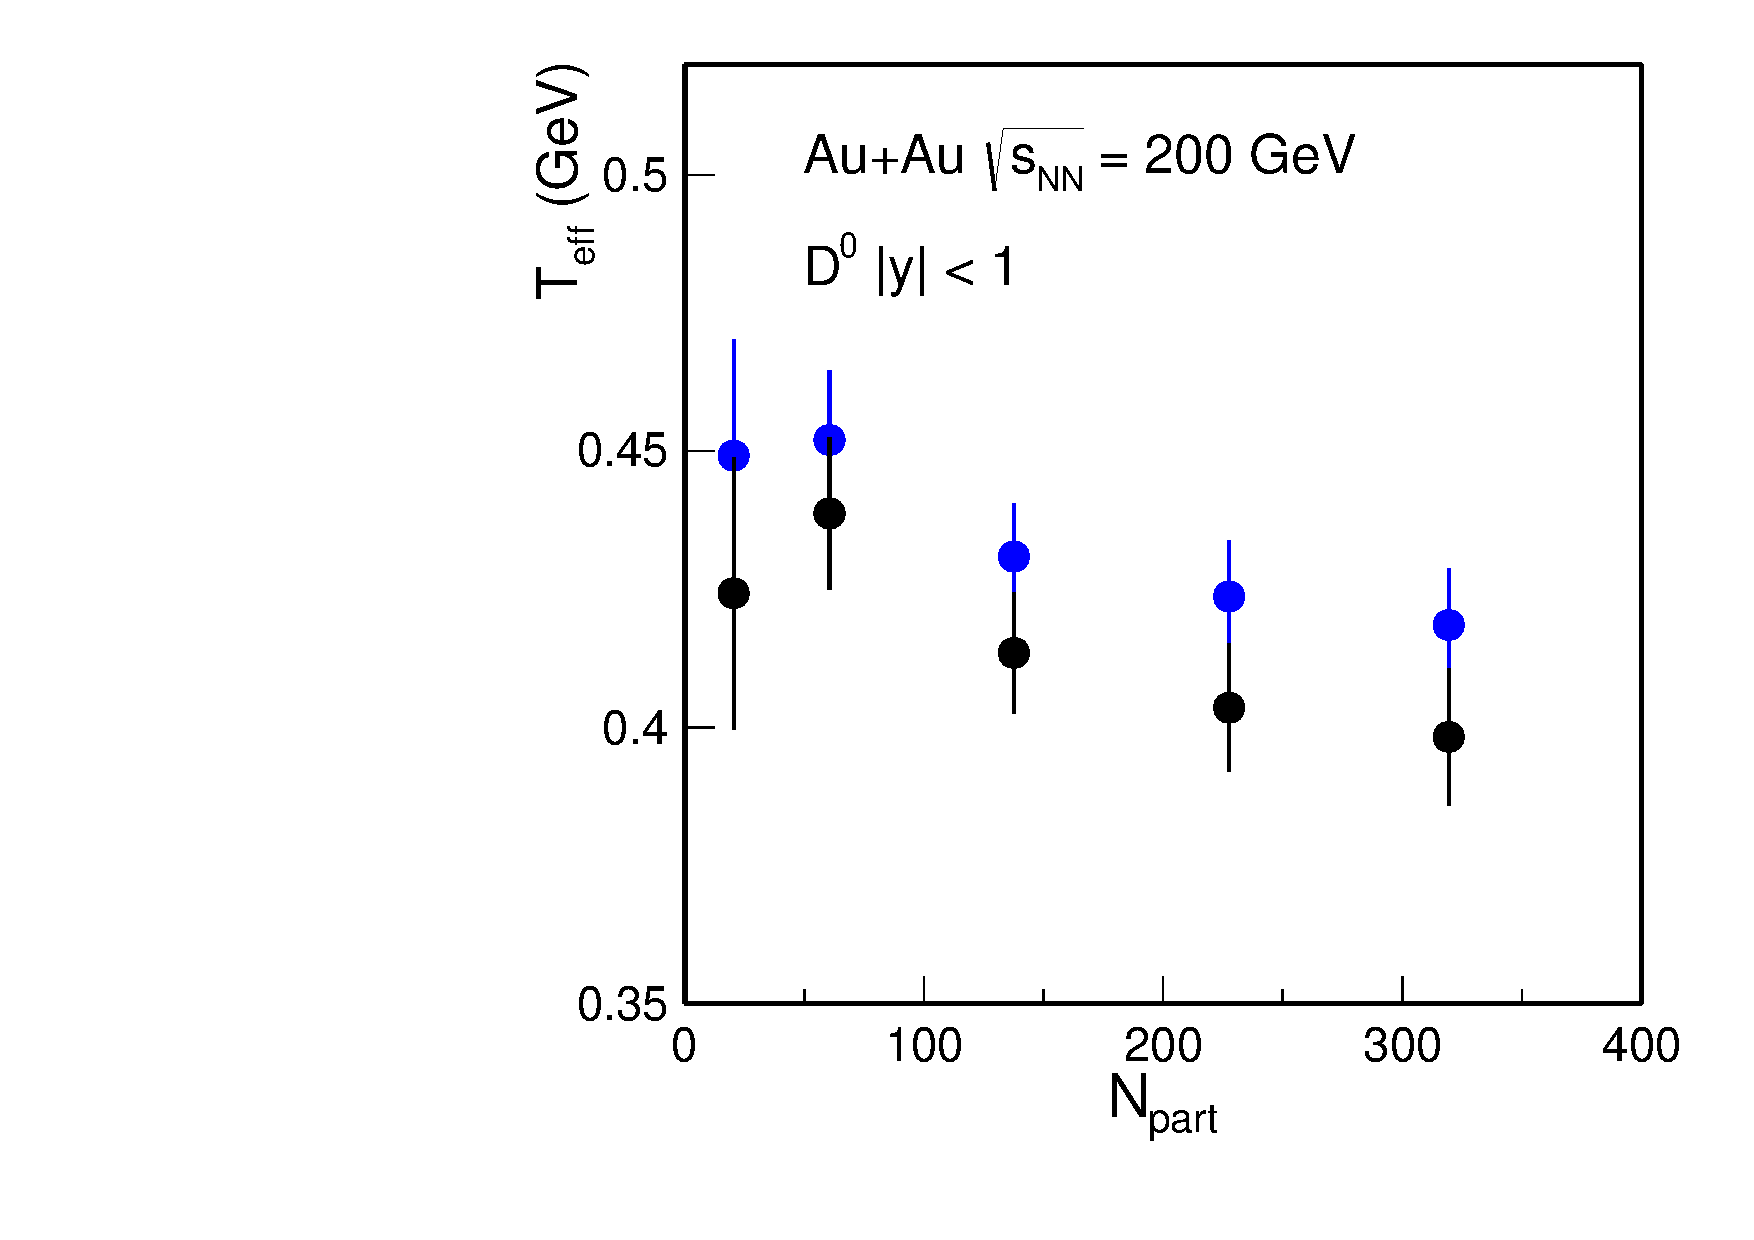
\includegraphics[width=0.48\textwidth]{fig/Teff_D0.pdf}
% \caption{$T_{eff}$ vs. $N_{bin}$ for different centrality classes in Au + Au collisions at $\sqrt{s_{_{\rm NN}}}$ = 200\,GeV.}
% \label{fig:Teff_D0} 
% \end{figure}

The obtained slope parameter $T_{\rm eff}$ for $D^0$ mesons is compared to other light and strange hadrons measured at RHIC. %Fig.~\ref{fig:mTFit_ALL} shows the exponential function fit to various hadron spectra 
Fig.~\ref{fig:Teff_ALL} summarizes the slope parameter $T_{\rm eff}$ for various identified hadrons ($\pi^{\pm}$, $K^{\pm}$, $p$/$\bar{p}$, $\phi$, $\Lambda$, $\Xi^-$, $\Omega$, $D^0$ and $J/\psi$) in central Au + Au collisions at $\sqrt{s_{_{\rm NN}}}$ = 200\,GeV. Point-by-point statistical and systematical uncertainties in the $m_{\rm T}$ spectra are added together in quadratic sum when performing these fits and error bars shown on the data points in this figure represent the total uncertainties. All fits are performed up to $m_{\rm T}$ - $m_{0}$ $<1$\,GeV/$c^2$ ($\pi,\ K,\ p$), $<2$\,GeV/$c^2$ ($\phi,\ \Lambda,\ \Xi$), $<3$\,GeV/$c^2$($\Omega,\ D^{0},\ J/\psi$) for each particle respectively. 

The slope parameter $T_{\rm eff}$ in a thermalized medium can be characterized by the random (generally interpreted as a kinetic freezeout temperature $T_{\rm fo}$) and collective (radial flow velocity $\langle\beta_{\rm T}\rangle$) components with a simple relation~\cite{StarWhitePaper,Csorgo:1995bi,Kolb:2003dz}

\[
T_{\rm eff} = T_{\rm fo} + m_0 \langle\beta_{\rm T}\rangle^2
\]

therefore, $T_{\rm eff}$ will show a linear dependence as a function of particle mass $m_0$ with a slope that can be used to characterize the radial flow collective velocity.

The data points show clearly two different systematic trends: $\pi,\ K,\ p$ data points follow one linear dependence while $\phi,\ \Lambda,\ \Xi^{-},\ \Omega^{-},\ D^0$ data points follow another linear dependence, as represented by the dashed lines shown in Fig.~\ref{fig:Teff_ALL}. Particles, such as, $\pi,\ K,\ p$ gain radial collectivity through the whole system evolution, therefore the linear dependence exhibits a larger slope. On the other hand the linear dependence of $\phi,\ \Lambda,\ \Xi^{-},\ \Omega^{-},\ D^0$ data points shows a smaller slope indicating these particles may freeze out from the system earlier, and therefore receive less radial collectivity.

% \begin{figure}
% \centering
% 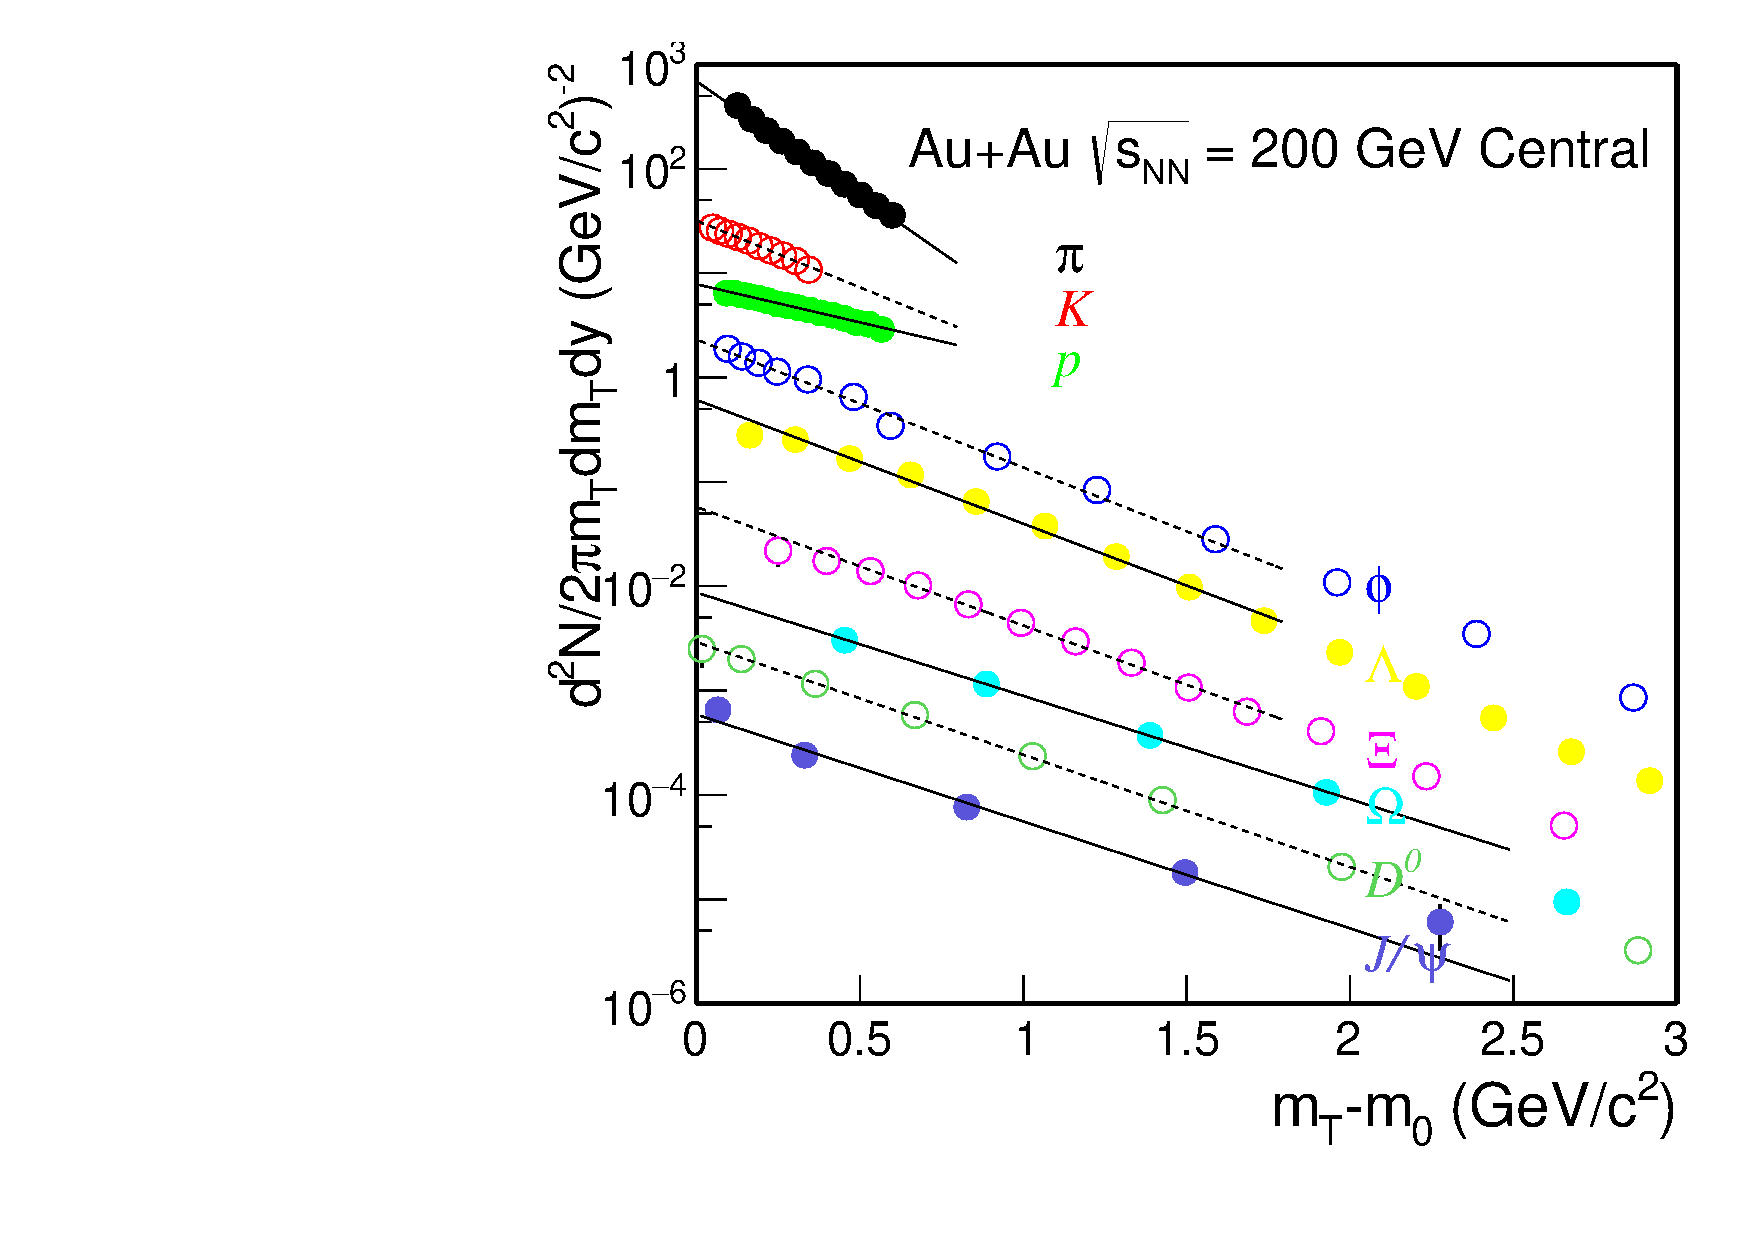
\includegraphics[width=0.5\textwidth]{fig/mTFit_ALL.pdf}
% \caption{$D^{0}$ invariant yield at mid-rapidity ($|y|<1$) vs. ($m_{T}$ - $m_{0}$) for central collisions in Au + Au collisions at $\sqrt{s_{_{\rm NN}}}$ = 200\,GeV.}
% \label{fig:mTFit_ALL} 
% \end{figure}

\begin{figure}
\centering
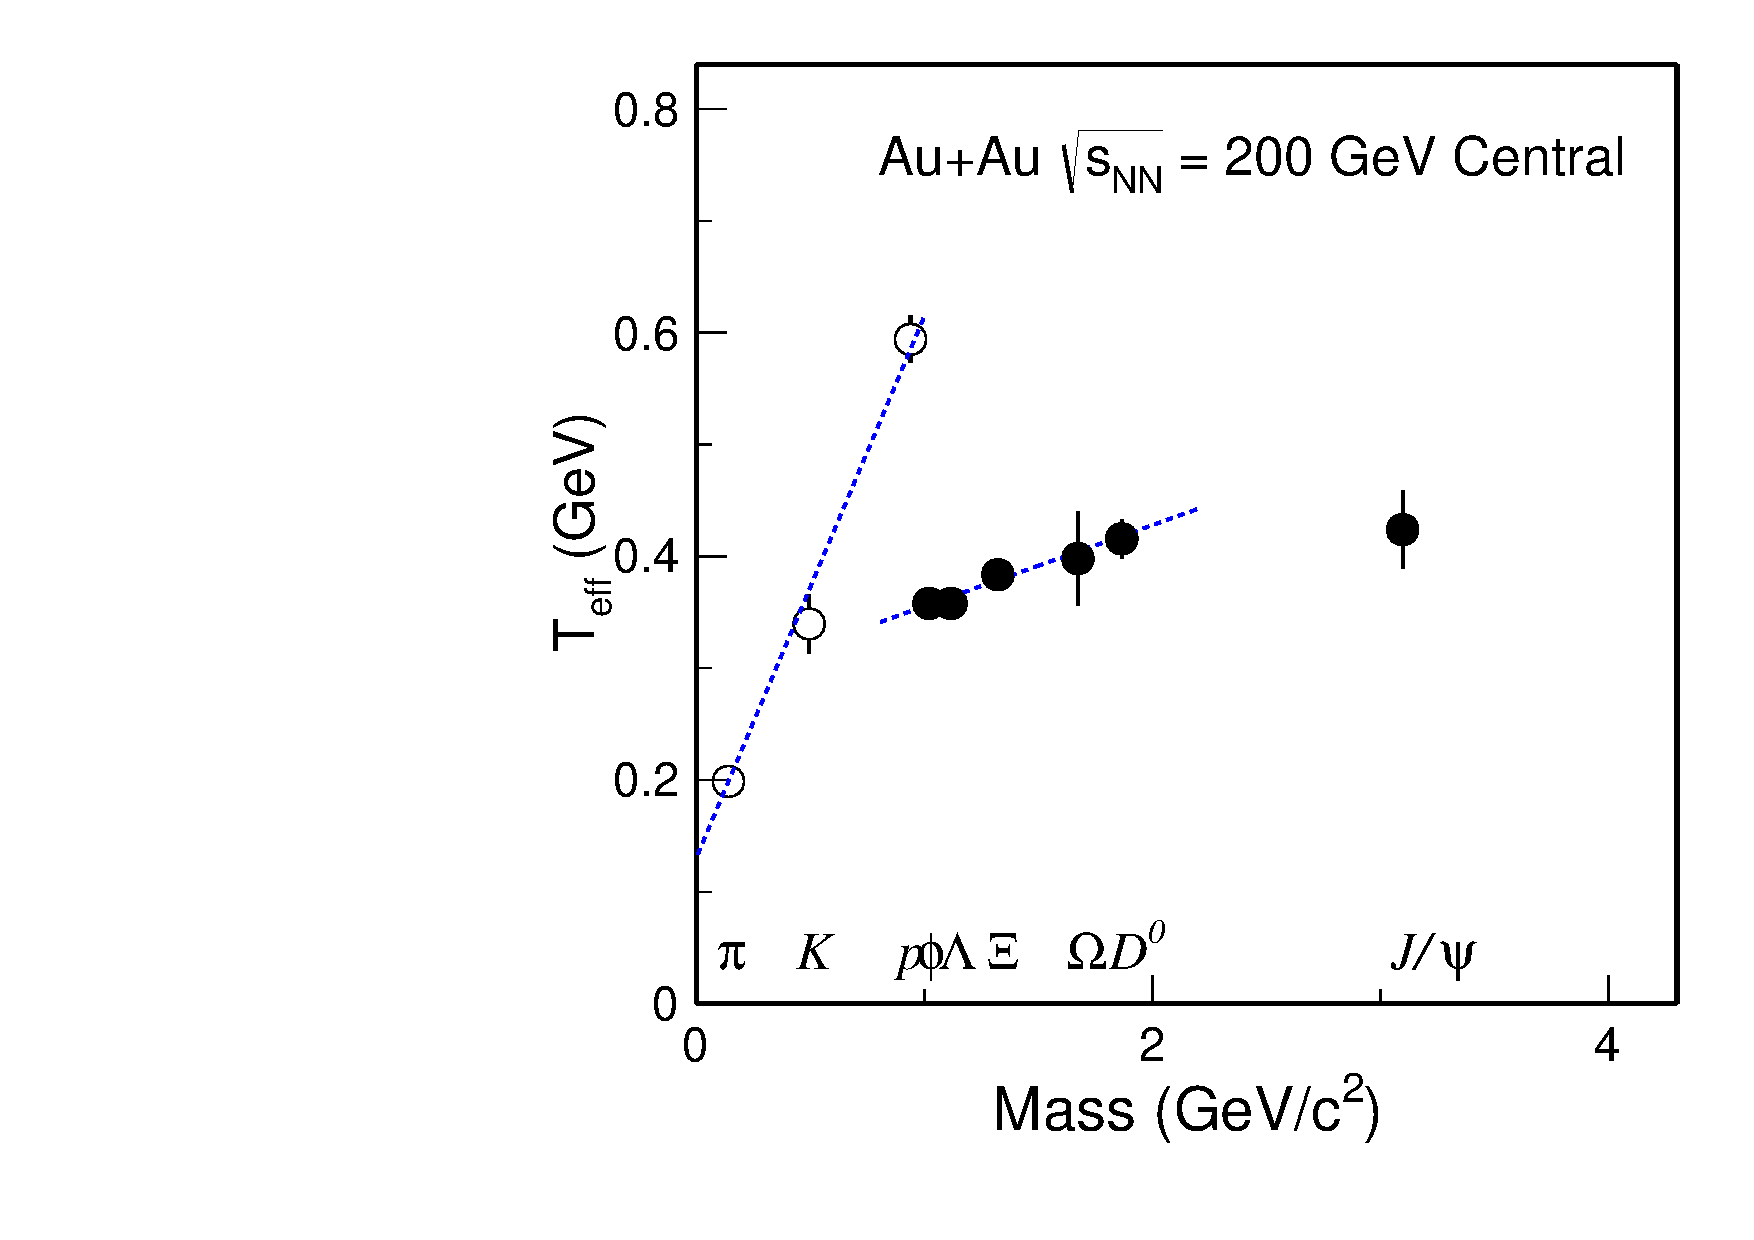
\includegraphics[width=0.43\textwidth]{fig/Teff_ALL.pdf}
% 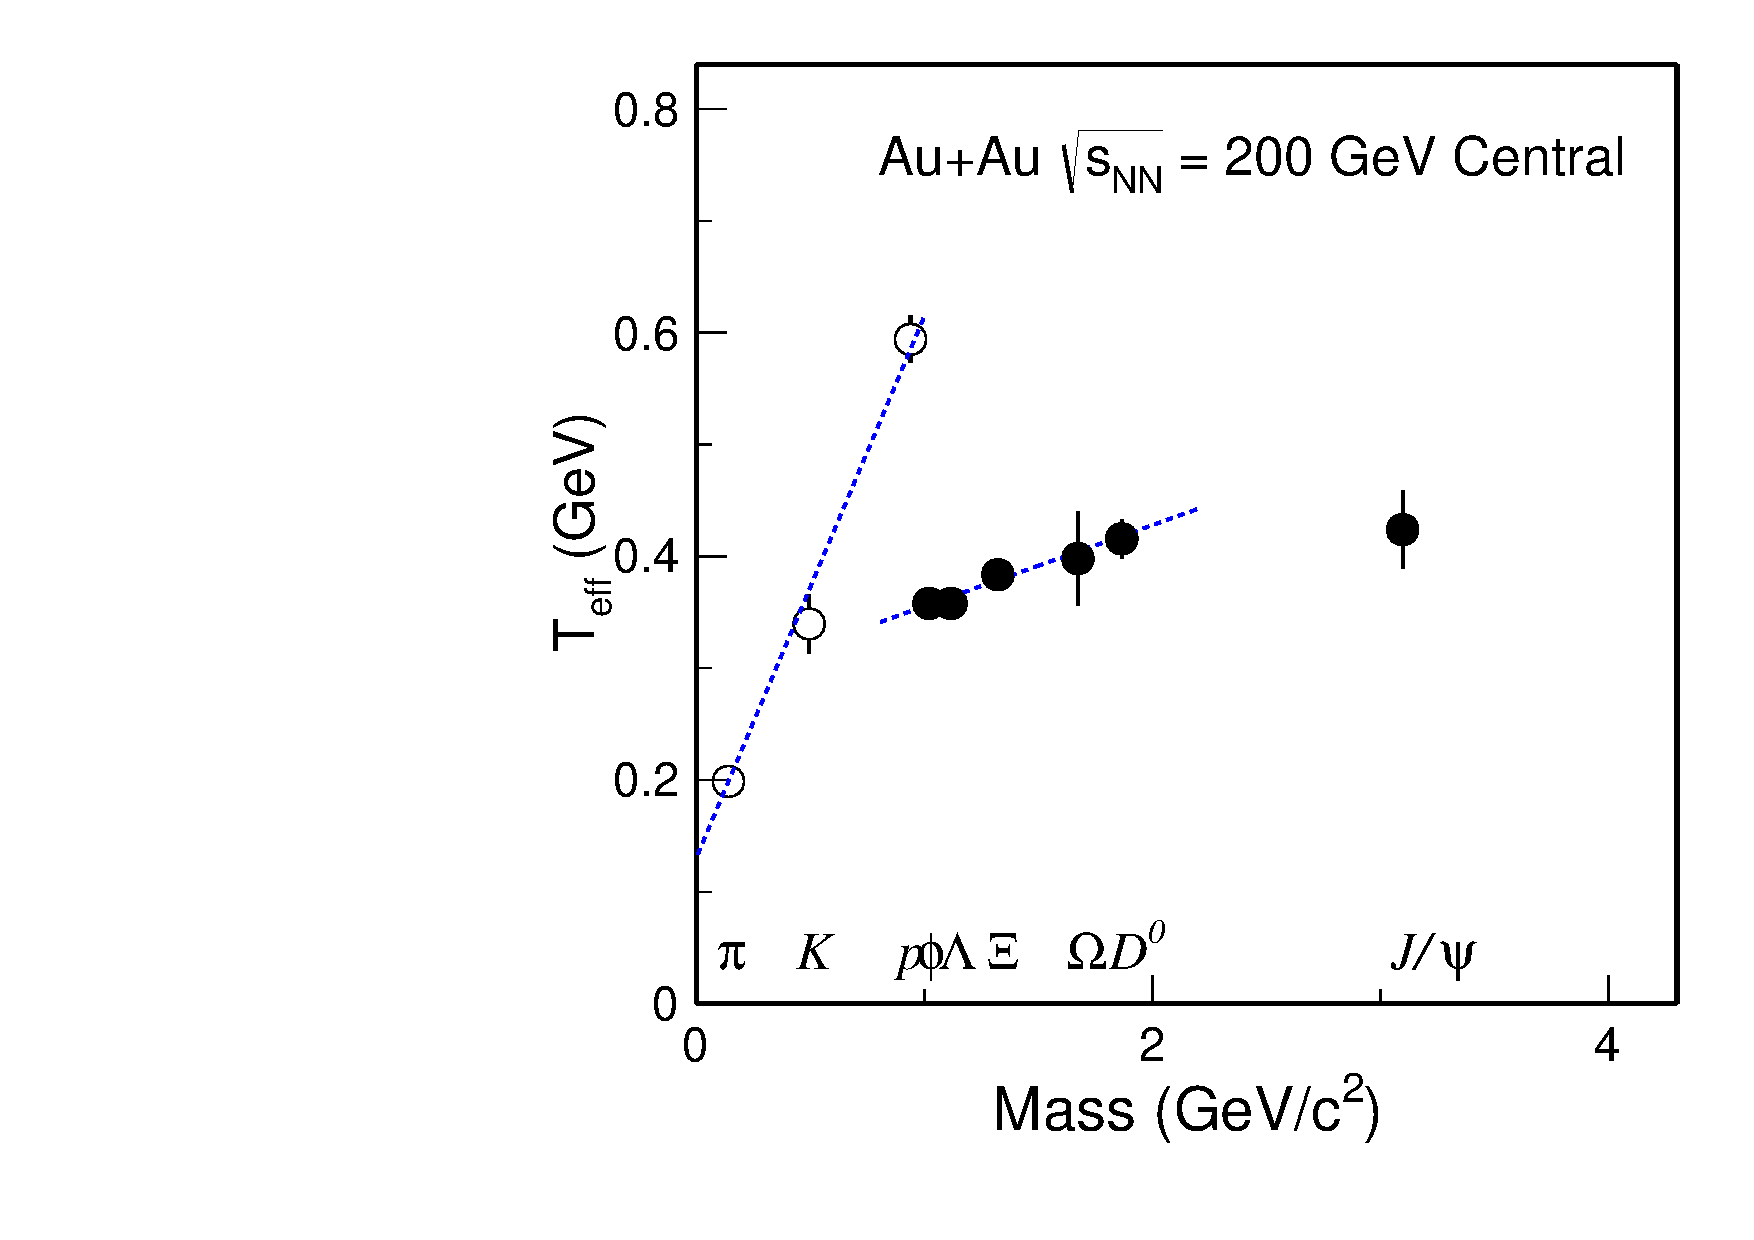
\includegraphics[width=0.4\textwidth]{fig/Teff_ALL.pdf}
\caption{Slope parameter $T_{\rm eff}$ for different particles in central Au + Au collisions at $\sqrt{s_{_{\rm NN}}}$ = 200\,GeV. The dashed lines depict linear function fits to $\pi,K,p$ and $\phi,\Lambda,\Xi^{-},\Omega^{-},D^0$ respectively.}
\label{fig:Teff_ALL} 
\end{figure}


\subsubsection{\label{result:collectivity:BW}Blast-wave fit}

\begin{figure}
\centering
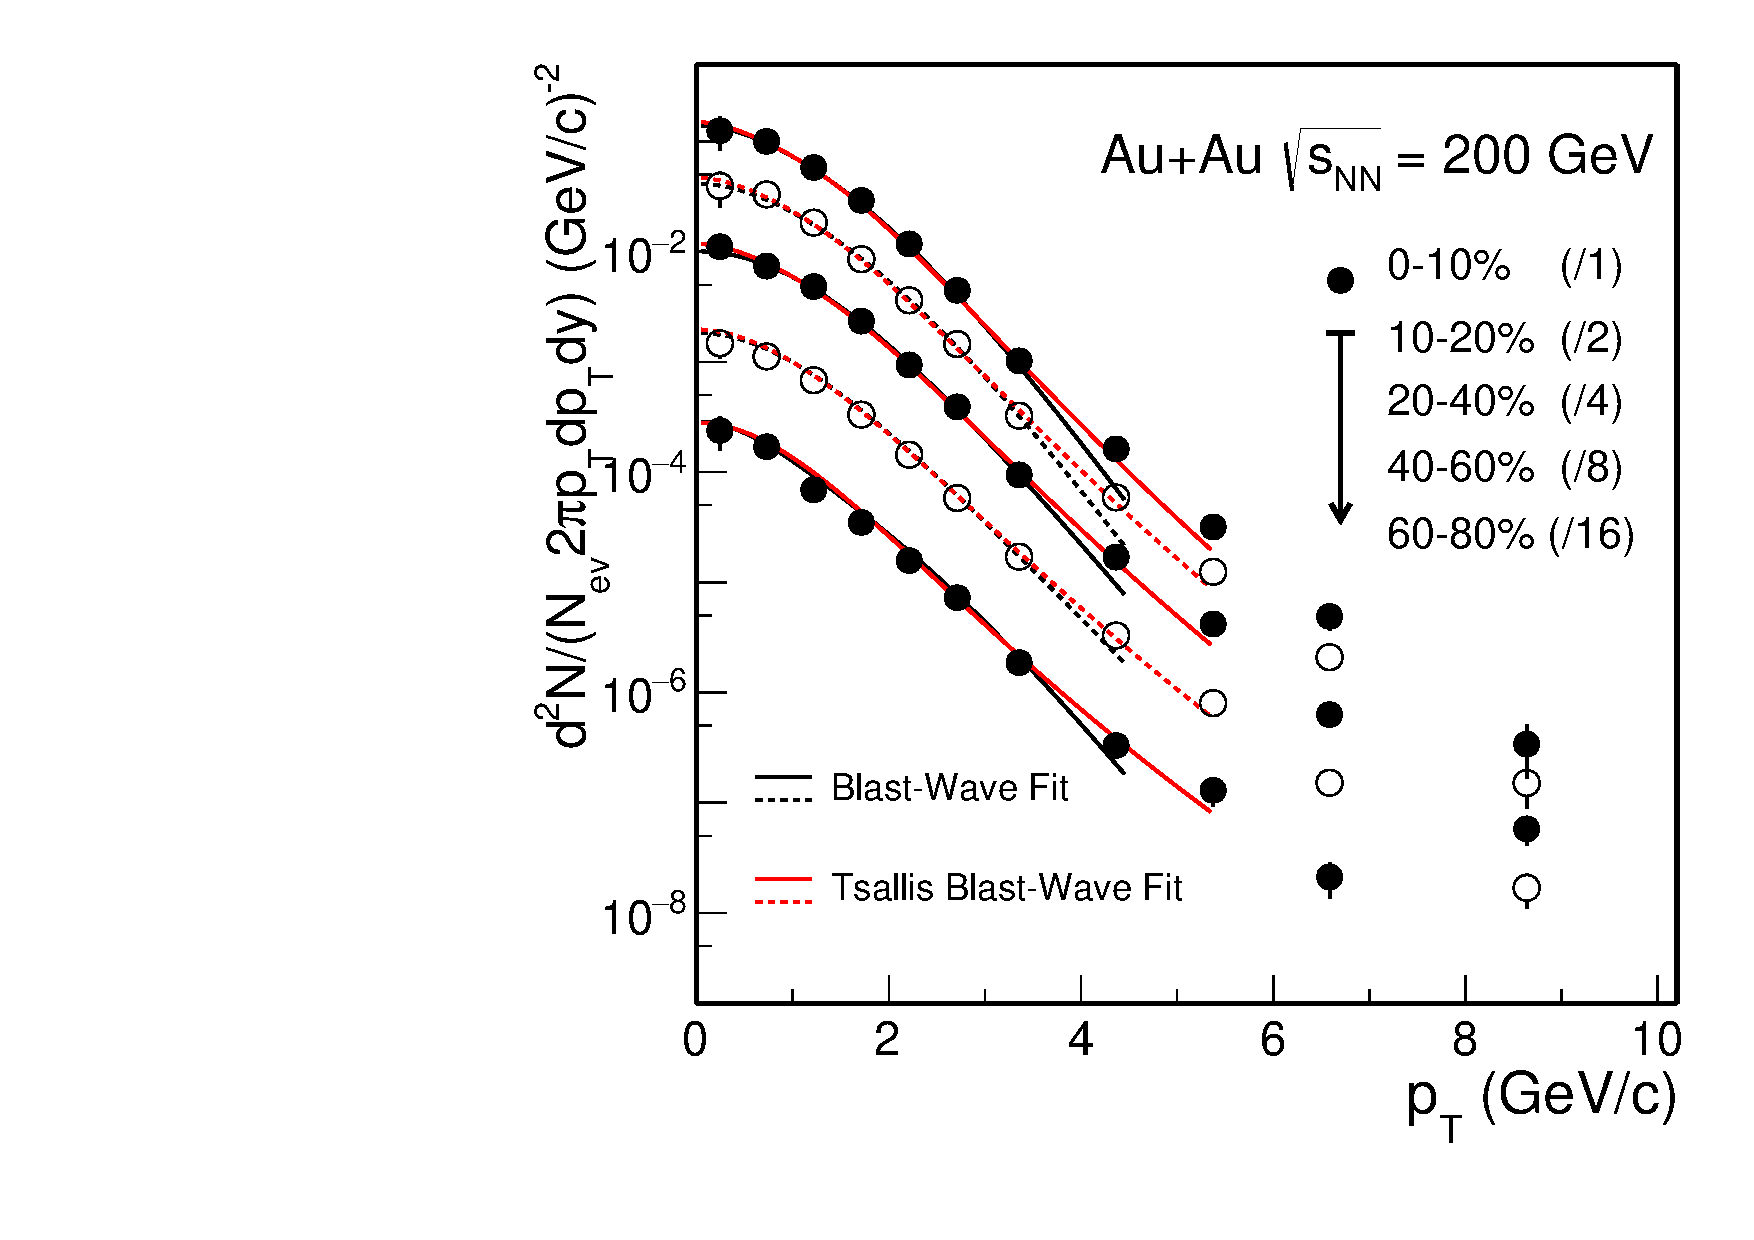
\includegraphics[width=0.43\textwidth]{fig/BWFit.pdf}
% 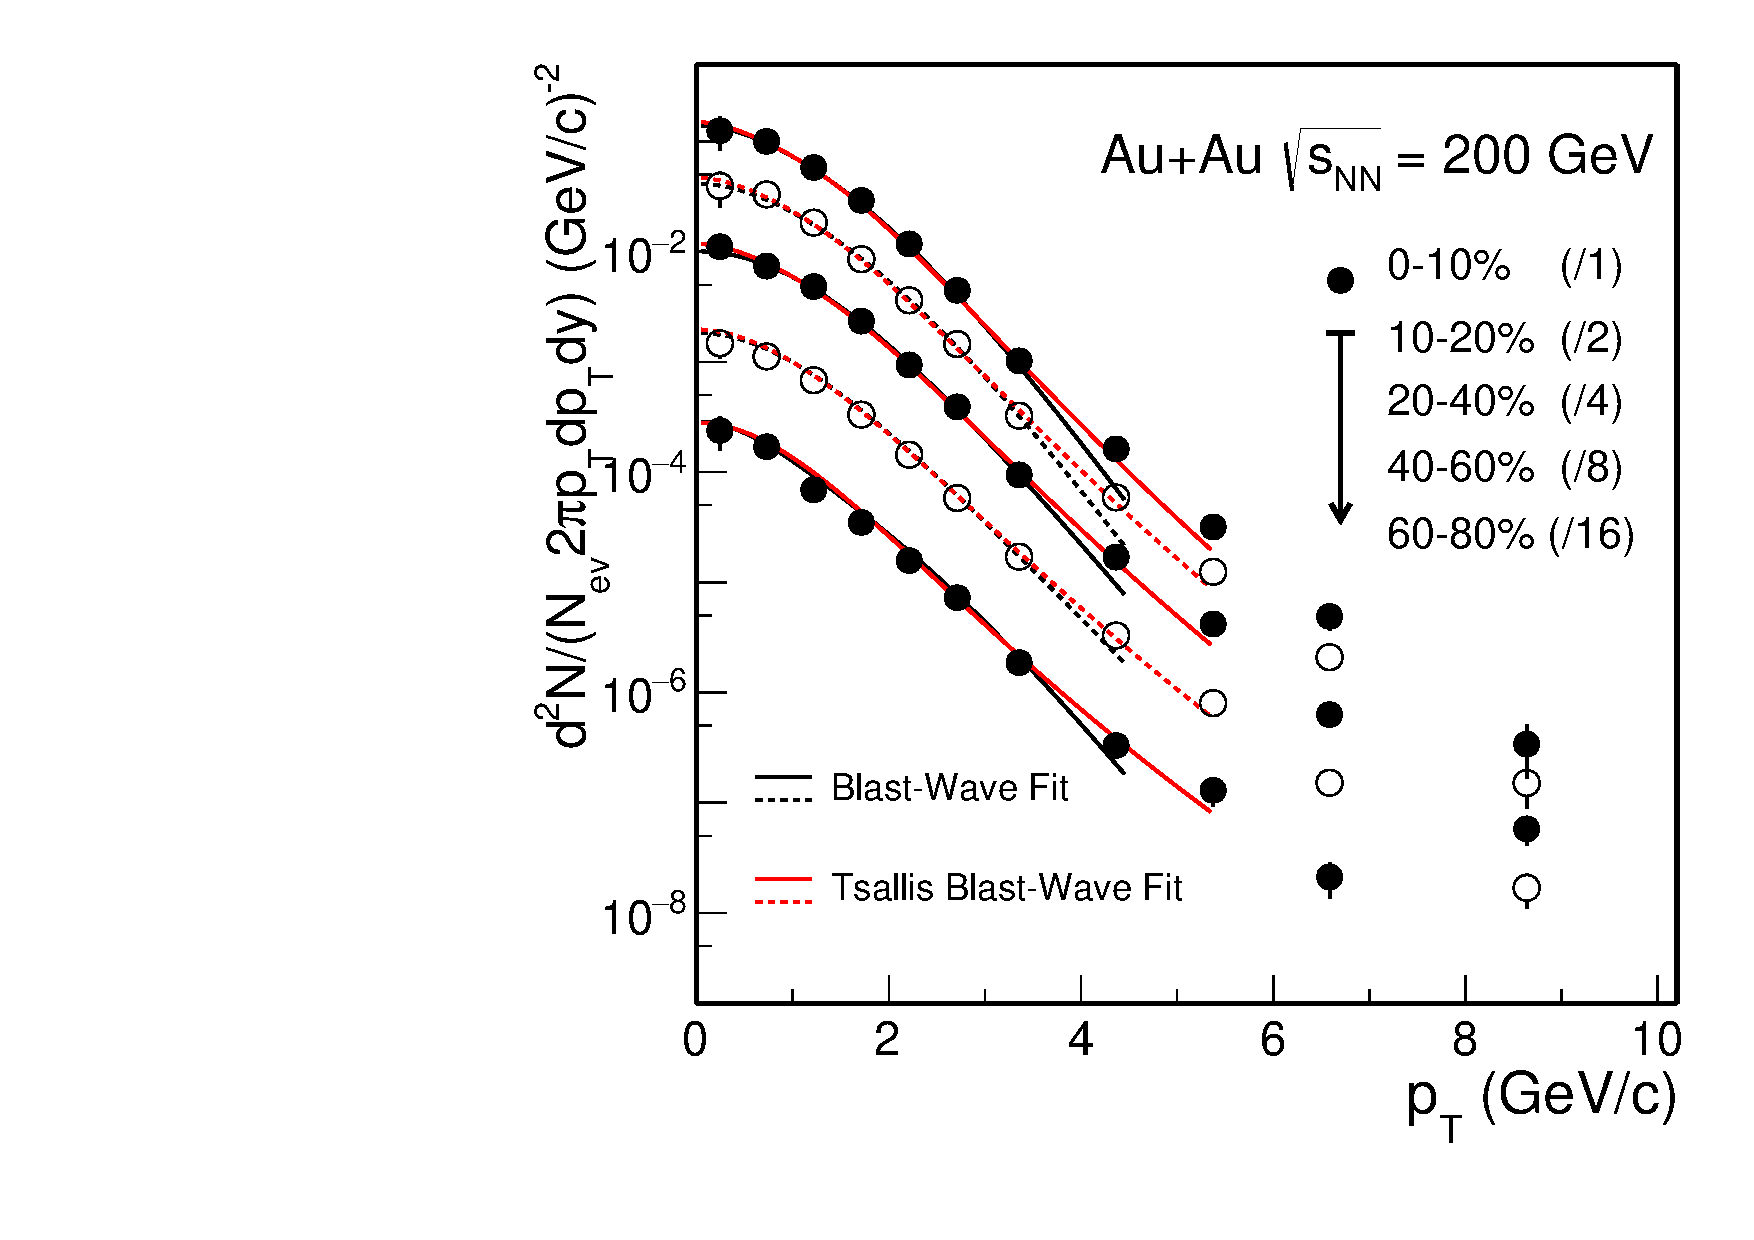
\includegraphics[width=0.4\textwidth]{fig/BWFit.pdf}
\caption{$D^{0}$ invariant yield at mid-rapidity ($|y|<1$) vs. transverse momentum for different centrality classes in Au + Au collisions at $\sqrt{s_{_{\rm NN}}}$ = 200\,GeV. Solid and dashed black lines depict Blast-Wave function and Tsallis Blast-Wave (TBW) fits.}
\label{fig:BWFit} 
\end{figure}

Blast-Wave (BW) model is extensively used to study the particle kinetic freeze-out properties. Assuming a hard-sphere uniform particle source with a kinetic freeze-out temperature $T_{\rm kin}$ and a transverse radial flow velocity $\beta$, the particle transverse momentum spectral shape is given by~\cite{Schnedermann:1993ws}

\begin{widetext}
\[
\frac{dN}{p_{\rm T}dp_{\rm T}} = \frac{dN}{m_{\rm T}dm_{\rm T}} \propto \int_0^R rdr m_{\rm T} I_0\bigg(\frac{p_{\rm T}\sinh\rho}{T_{\rm kin}}\bigg) K_1\bigg(\frac{m_{\rm T}\cosh\rho}{T_{\rm kin}}\bigg)
\]
\end{widetext}
where $\rho = \tanh^{-1}\beta$, and $I_0$ and $K_1$ are the modified Bessel functions. The flow velocity profile is taken as

\[
\beta = \beta_{\rm S}\left(\frac{r}{R}\right)^{n}
\]

where $\beta_{\rm S}$ is the maximum velocity at the surface and $r/R$ is the relative radial position in the thermal source. The choice of $R$ only affects the overall spectrum magnitude while the spectrum shape constrains the three free parameters $T_{\rm kin}$, $\langle\beta\rangle=2/(2+n)\beta_{\rm S}$ and $n$.

% To account for the degree of non-equilibrium, Tsallis statistics has been introduced into the Blast-wave model with an additional parameter $q-1$~\cite{Tang:2008ud}, and the Blast-Wave distribution can be modified as
% \begin{widetext}
% \[
% \frac{dN}{m_{\rm T}dm_{\rm T}} \propto m_{\rm T}\int_{-Y}^{+Y}\cosh(y)dy \int_{-\pi}^{+\pi} d\phi \int_0^R rdr \bigg(1+\frac{q-1}{T_{\rm kin}}\big(m_{\rm T}\cosh(y)\cosh(\rho)-p_{\rm T}\sinh(\rho)\cos(\phi)\big)\bigg)^{\textstyle -\frac{1}{q-1}}
% \]
% \end{widetext}
% In the limit of $q\rightarrow 1$, the TBW distribution returns to the regular Blast-Wave one. The new Tsallis Blast-Wave (TBW) model has been used to fit the RHIC light and strange hadron spectra and it shows nice description of these particle spectra up to 3 GeV/$c$.
%

Figure~\ref{fig:BWFit} shows the Blast-Wave and Tsallis Blast-Wave (TBW)~\cite{Tang:2008ud} fits to the data in different centrality bins, respectively. The $n$ parameter in these fit is fixed to be 1 due to the limited number of data points and also inspired by the fit result for light flavor hadrons ($\pi,K,p$). The $p_{\rm T}$ range in the BW fits is restricted to be less than 3$m_{0}$ where $m_{0}$ is the rest mass of $D^0$ mesons.

\begin{figure}
\centering
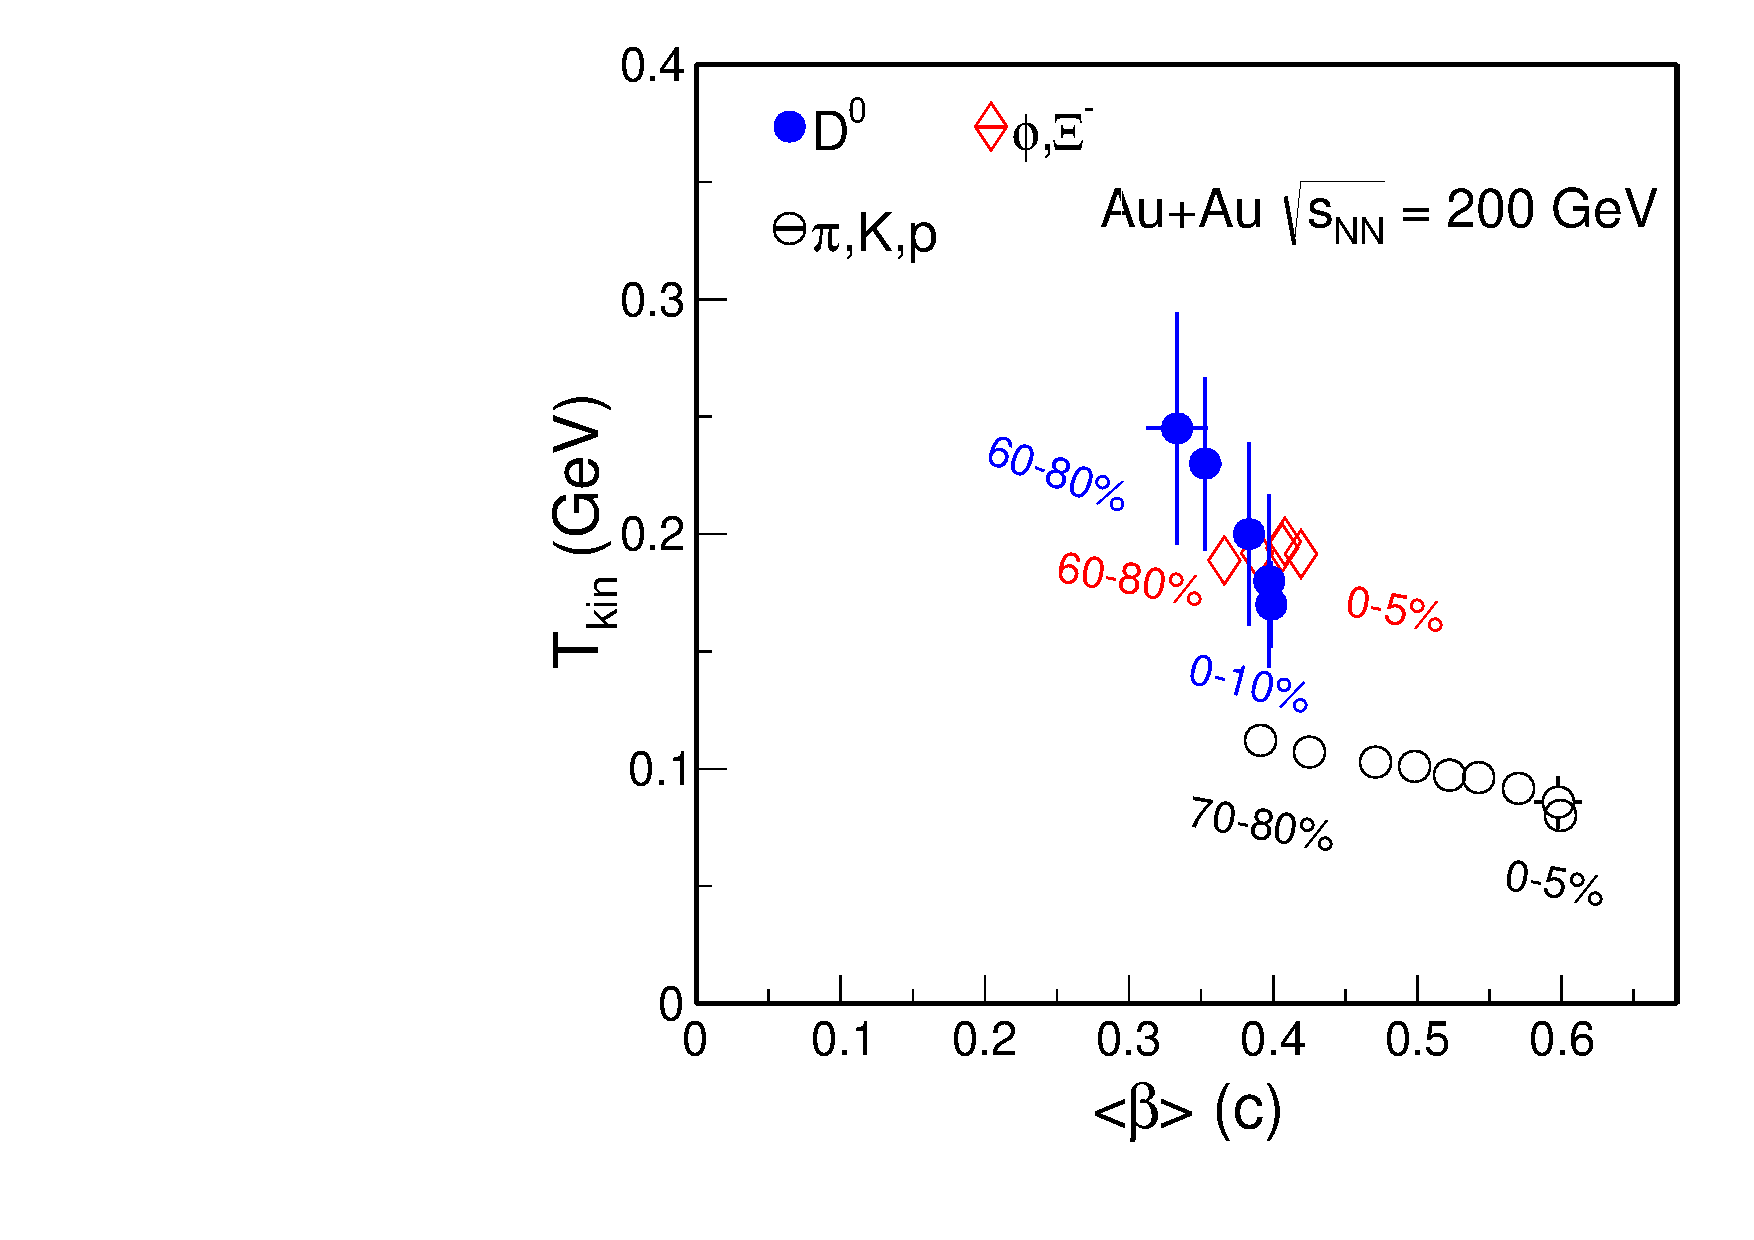
\includegraphics[width=0.43\textwidth]{fig/TvsBeta.pdf}
\caption{$T_{\rm kin}$ vs. $\langle\beta\rangle$ from the Blast-Wave model fits to different groups of particles. The data points for each group of particles present the results from different centrality bins with the most central data point at the largest $\langle\beta\rangle$.}
\label{fig:BWFitSummary} 
\end{figure}

Figure~\ref{fig:BWFitSummary} summarizes the fit parameters $T_{\rm kin}$ vs. $\langle\beta\rangle$ from the Blast-Wave model fits to different group of particles: black markers for the simultaneous fit to $\pi,\ K,\ p$, red markers for the simultaneous fit to $\phi,\ \Xi^-$ and blue markers for the fit to $D^0$. The data points for each group of particles represent the fit results from different centrality bins with the most central data point at the largest $\langle\beta\rangle$ value. Similar as in the fit to $m_{\rm T}$ spectra, point-by-point statistical and systematical uncertainties on the measured $p_{\rm T}$ spectra are added in quadratic when performing the fit. The fit results for $\pi,\ K,\ p$ are consistent with previously published results~\cite{Tang:2008ud}. The fit results for multi-strangeness particles $\phi,\ \Xi^{-}$ and $D^0$ show much smaller mean transverse velocity $\langle\beta\rangle$ and larger kinetic freeze-out temperature. This is also consistent with that these particles freeze out from the system earlier and gain less radial collectivity. The resulting $T_{\rm kin}$ parameters for $\phi,\ \Xi^-$ and for $D^0$ are close to the critical temperature $T_{\rm C}$ (of about 160 MeV) indicating negligible contribution from the hadronic stage to the observed radial flow of these particles. The collectivity they obtain are mostly through the partonic stage re-scatterings in the QGP phase. 

The TBW fit accounts for non-equilibrium feature in a system with an additional parameter $q$~\cite{Tang:2008ud}. %Table~\ref{table:TBW_fit} 
Table VI lists the fitting parameters, $\langle\beta\rangle$ and $(q-1)$ for the $D^0$ data in different centralities. Results show a similar trend as the regular BW fit, i.e. the most central data point locates at the largest $\langle\beta\rangle$ value. The $(q-1)$ parameter in TBW, which characterizes the degree of non-equilibrium in a system, indicates decreasing trend from peripheral to central collisions, indicating that the system is approaching towards thermalization in more central collisions.
% Qualitatively, increasing centrality produces a strong increase in flow velocity, a mild increase in temperature, and a dramatic decrease in (q−1). This is consistent with a picture of increased thermalization with centrality but disfavors complete thermal equilibrium in all systems.

\begin{table}[t]
\centering{
  \caption{ $\langle\beta\rangle$ and $(q-1)$ from the Tsallis Blast-Wave fits to the $D^0$ data in different centralities .}
\begin{tabular}{rcccccccc} \hline \hline
  \hspace{1cm}Centrality\hspace{1cm} & \multicolumn{3}{c}{$\langle\beta\rangle$($c$)} & & \multicolumn{3}{c}{$q-1$} & \hspace{1cm} \\ \hline
  0--10 \%\hspace{1cm}     & 0.263 & $\pm$ & 0.018 & & 0.066 & $\pm$ & 0.008 \\
  10--20 \%\hspace{1cm}    & 0.255 & $\pm$ & 0.022 & & 0.068 & $\pm$ & 0.010 \\
  20--40 \%\hspace{1cm}    & 0.264 & $\pm$ & 0.015 & & 0.070 & $\pm$ & 0.007 \\
  40--60 \%\hspace{1cm}    & 0.251 & $\pm$ & 0.023 & & 0.074 & $\pm$ & 0.011 \\
  60--80 \%\hspace{1cm}    & 0.217 & $\pm$ & 0.037 & & 0.075 & $\pm$ & 0.010  \\ \hline \hline
\end{tabular}
}
\label{table:TBW_fit}
\end{table}

\subsection{\label{result:RCP}Nuclear Modification Factor - $R_{\rm CP}$ $\&\&$  $R_{\rm AA}$}

\begin{figure}
\centering
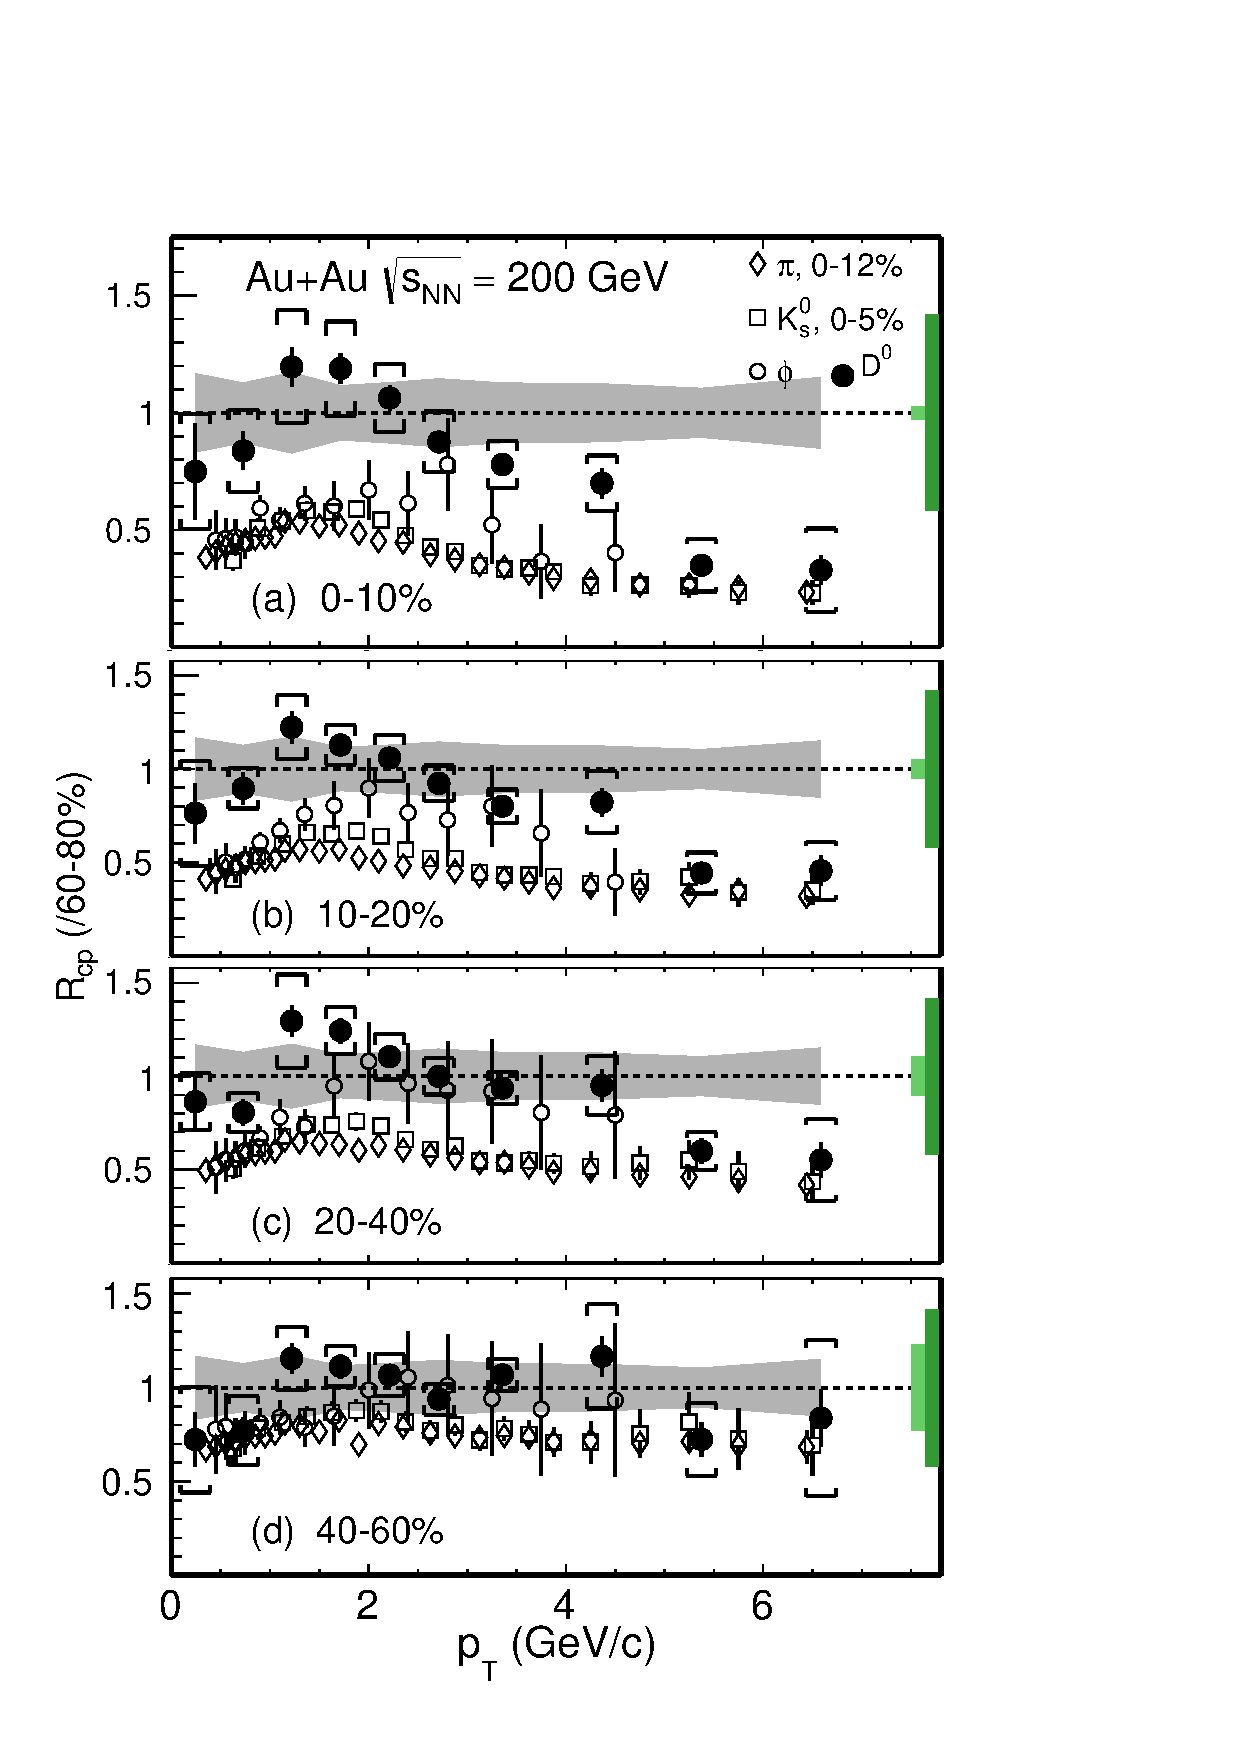
\includegraphics[width=0.45\textwidth]{fig/D0_Rcp1.pdf}
\caption{$D^{0}$ $R_{\rm CP}$ with the 60--80\% spectrum as the reference for different centrality classes in Au + Au collisions at $\sqrt{s_{_{\rm NN}}}$ = 200\,GeV compared to that of other light and strange mesons ($\pi^{\pm}$, $K^0_{S}$ and $\phi$)~\cite{Adams2006_Identified,Abelev2009,Agakishiev2012}. The statistical and systematic uncertainties are shown as error bars and brackets on the data points. The grey bands around unity depict the systematic uncertainty due to vertex resolution correction, mostly from the 60--80\% reference spectrum. The light and dark green boxes on the right depict the normalization uncertainty in determining the $N_{\rm bin}$.}
\label{fig:D0_Rcp} 
\end{figure}

Figure~\ref{fig:D0_Rcp} shows the calculated $R_{\rm CP}$ with the 60--80\% peripheral bin as the reference for different centrality bins 0--10\%, 10--20\%, 20--40\% and 40--60\% and compared to other light and strange flavor mesons. The grey bands around unity depict the vertex resolution correction uncertainty on the measured $D^0$ data points, mostly originating from the 60--80\% reference spectrum. The dark and light green boxes around unity on the right side indicate the global $N_{\rm bin}$ systematic uncertainties for the 60--80\% centrality bin and for the corresponding centrality bin in each panel. The global $N_{\rm bin}$ systematic uncertainties should be applied to the data points of all particles in each panel.

The measured $D^0$ $R_{\rm CP}$ in central 0--10\% collisions shows a significant suppression at $p_{\rm T}>$ 5\,GeV/$c$. The suppression level is similar to that of light and strange flavor mesons and the $R_{\rm CP}$ suppression gradually descreses when moving towards mid-central and peripheral collisions. At $p_{\rm T}<4$\,GeV/$c$, the $D^0$ $R_{\rm CP}$ is higher than those of light flavor hadrons $\pi^{\pm}$ and $K_{S}^0$. This structure is consistent with the expectation from model predictions that charm quarks gain sizable collectivity during the medium evolution. Comparisons to dynamic model calculations for the $D^0$ $R_{\rm CP}$ will be discussed in the next section.

\begin{figure}
\centering
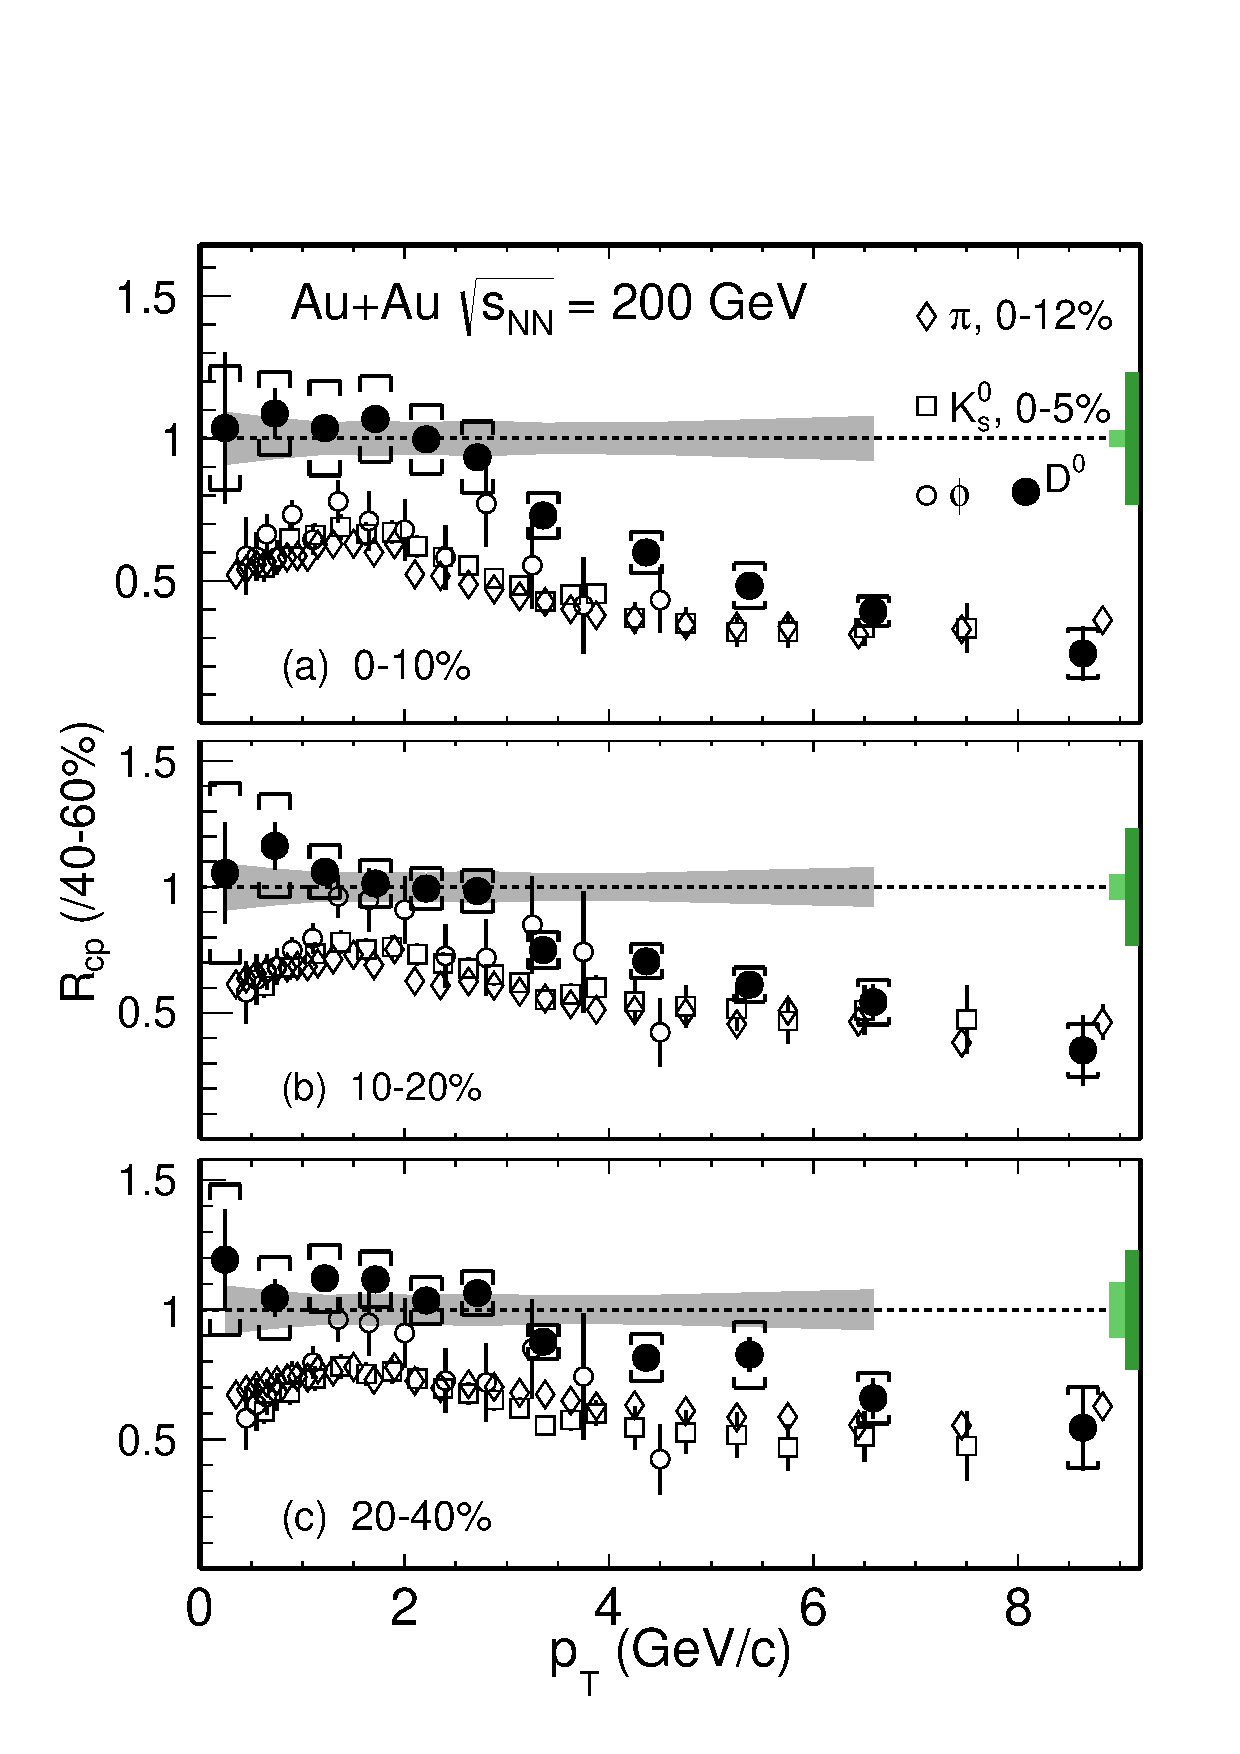
\includegraphics[width=0.45\textwidth]{fig/D0_Rcp2.pdf}
\caption{$D^{0}$ $R_{\rm CP}$ with the 40--60\% spectrum as the reference for different centrality classes in Au + Au collisions at $\sqrt{s_{_{\rm NN}}}$ = 200\,GeV compared to that of other light and strange mesons ($\pi^{\pm}$, $K^0_{S}$ and $\phi$)~\cite{Adams2006_Identified,Abelev2009,Agakishiev2012}. The statistical and systematic uncertainties are shown as error bars and brackets on the data points. The grey bands around unity depict the systematic uncertainty due to vertex resolution correction, mostly from the 40--60\% reference spectrum. The light and dark green boxes on the right depict the normalization uncertainty in determining the $N_{\rm bin}$.}
\label{fig:D0_Rcp2} 
\end{figure}

The precision of 60--80\% centrality spectrum is limited due to the large systematic uncertainty in determining the $N_{\rm bin}$ based on the MC Glauber model. Fig.~\ref{fig:D0_Rcp2} shows the $D^0$ $R_{\rm CP}$ for different centralities as a function of $p_{\rm T}$ with the 40--60\% centrality spectrum as the reference. The grey band around unity in the top panel is the vertex contribution for the systematic uncertainties from the 40--60\% centrality. The green boxes around unity depict the global $N_{\rm bin}$ systematic uncertainties for the 40--60\% centrality bin and for each corresponding centrality bin. As a comparison, $R_{\rm CP}$ of charged pions, $K_{s}^{0}$ and $\phi$ in the corresponding centralities are also plotted in each panel. With much smaller systematic uncertainties, the observations seen before using the 60--80\% centrality spectrum as the reference still hold. 


% \begin{figure}
% \centering
% 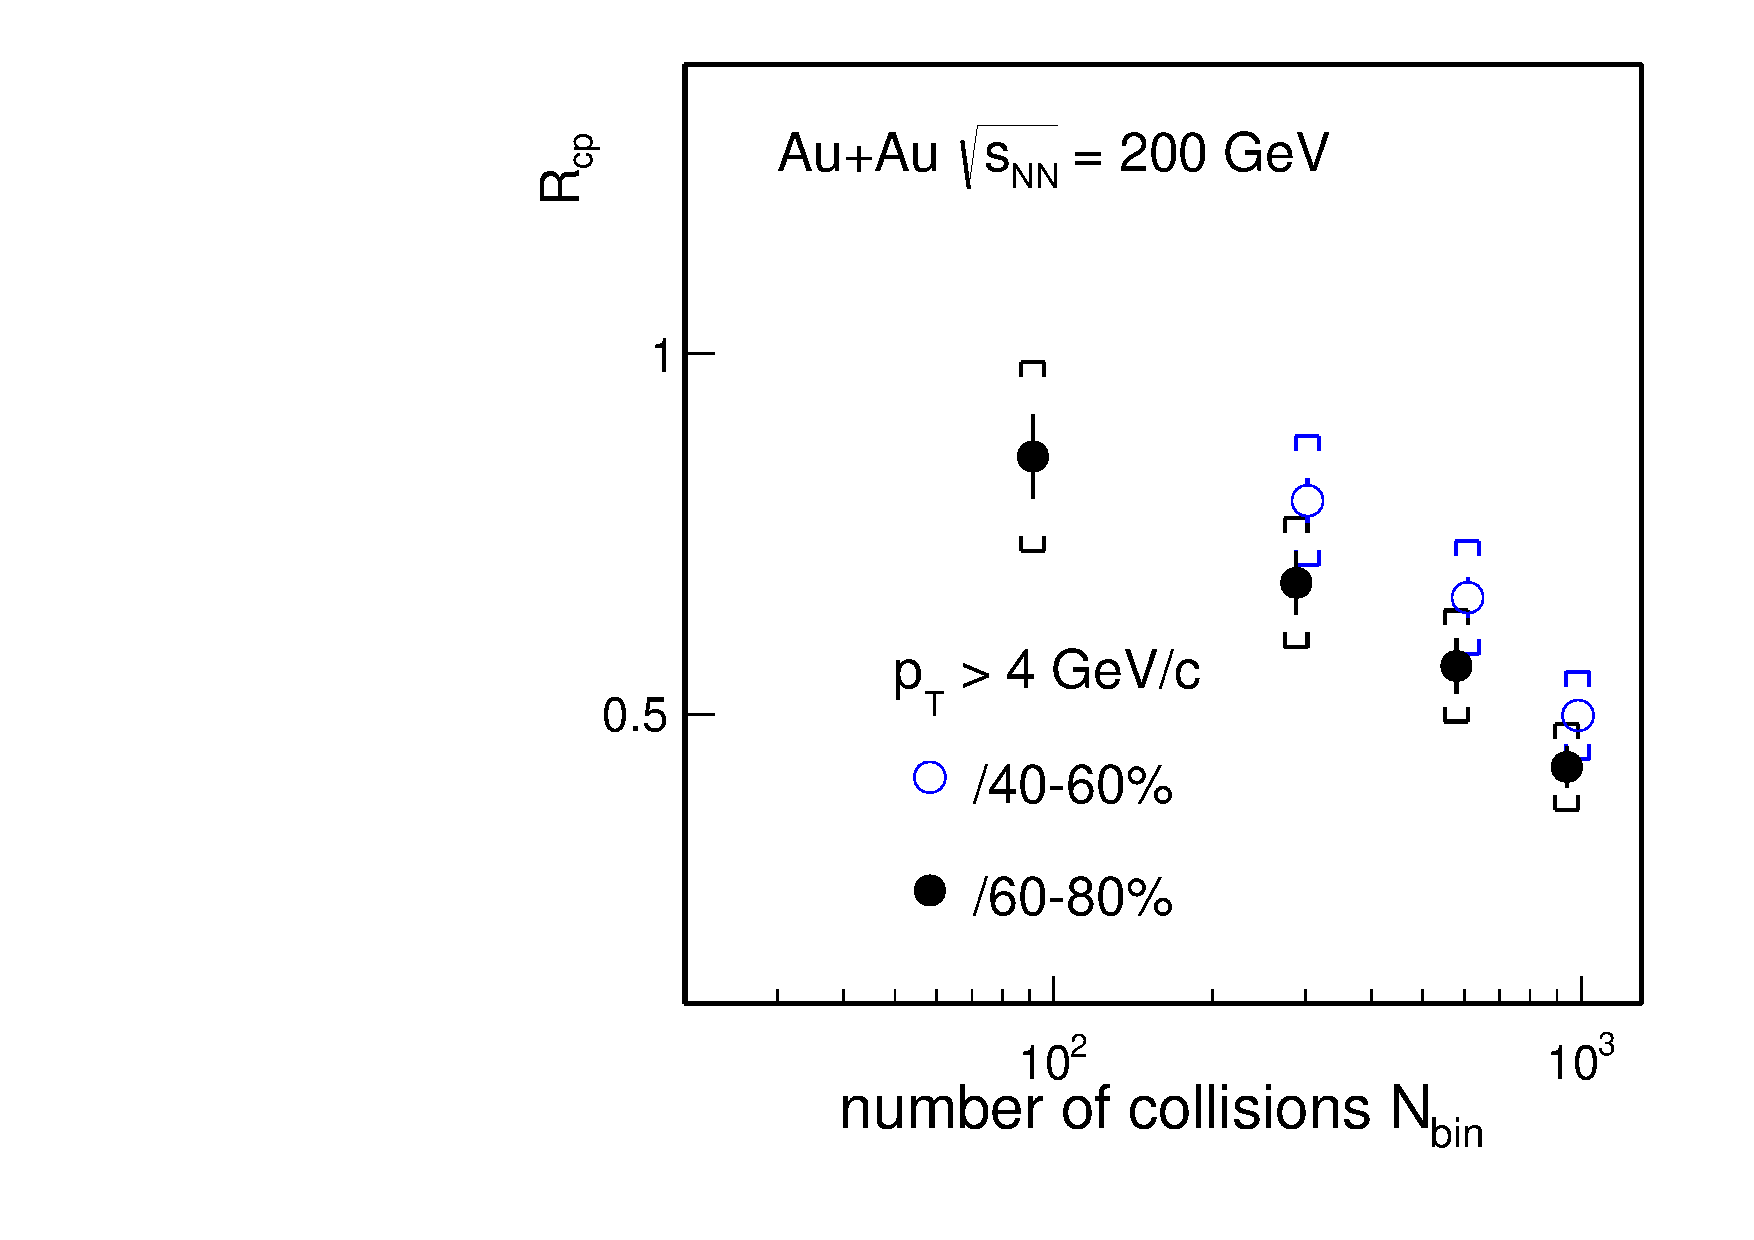
\includegraphics[width=0.48\textwidth]{fig/Rcp_Nbin_D0_2.pdf}
% \caption{$D^{0}$ $R_{cp}$ vs. $N_{bin}$ in Au + Au collisions.}
% \label{fig/Rcp_Nbin_D0_2} 
% \end{figure}

\begin{figure}
\centering
\includegraphics[width=0.45\textwidth]{fig/D0_RAA.eps}
% \caption{$D^{0}$ $R_{\rm AA}$ with the $p+p$ spectrum as the reference for different centrality classes in Au + Au collisions at $\sqrt{s_{_{\rm NN}}}$ = 200\,GeV. The first two and last two data points are empty circles indicating that those are unmeasured $p_{\rm T}$ range from $p+p$. The statistical and systematic uncertainties are shown as error bars and brackets on the data points for Au + Au. The grey bands around each data point depict the systematic uncertainty from $p+p$ reference spectrum. The light and dark green boxes on the right depict the normalization uncertainty in determining the $N_{\rm bin}$ and cross section from $p+p$.}
\caption{$D^{0}$ $R_{\rm AA}$ with the $p+p$ spectrum as the reference for different centrality classes in Au + Au collisions at $\sqrt{s_{_{\rm NN}}}$ = 200\,GeV. The first two and last two data points are presented as empty circles, indicating that the $p+p$ reference is extrapolated into these $p_T$ ranges. The statistical and systematic uncertainties are shown as error bars and brackets on the data points. The light and dark green boxes on the right depict the normalization uncertainty in determining the $N_{\rm bin}$ and cross section from $p+p$.}
\label{fig:D0_RAA} 
\end{figure}

\begin{figure}
\centering
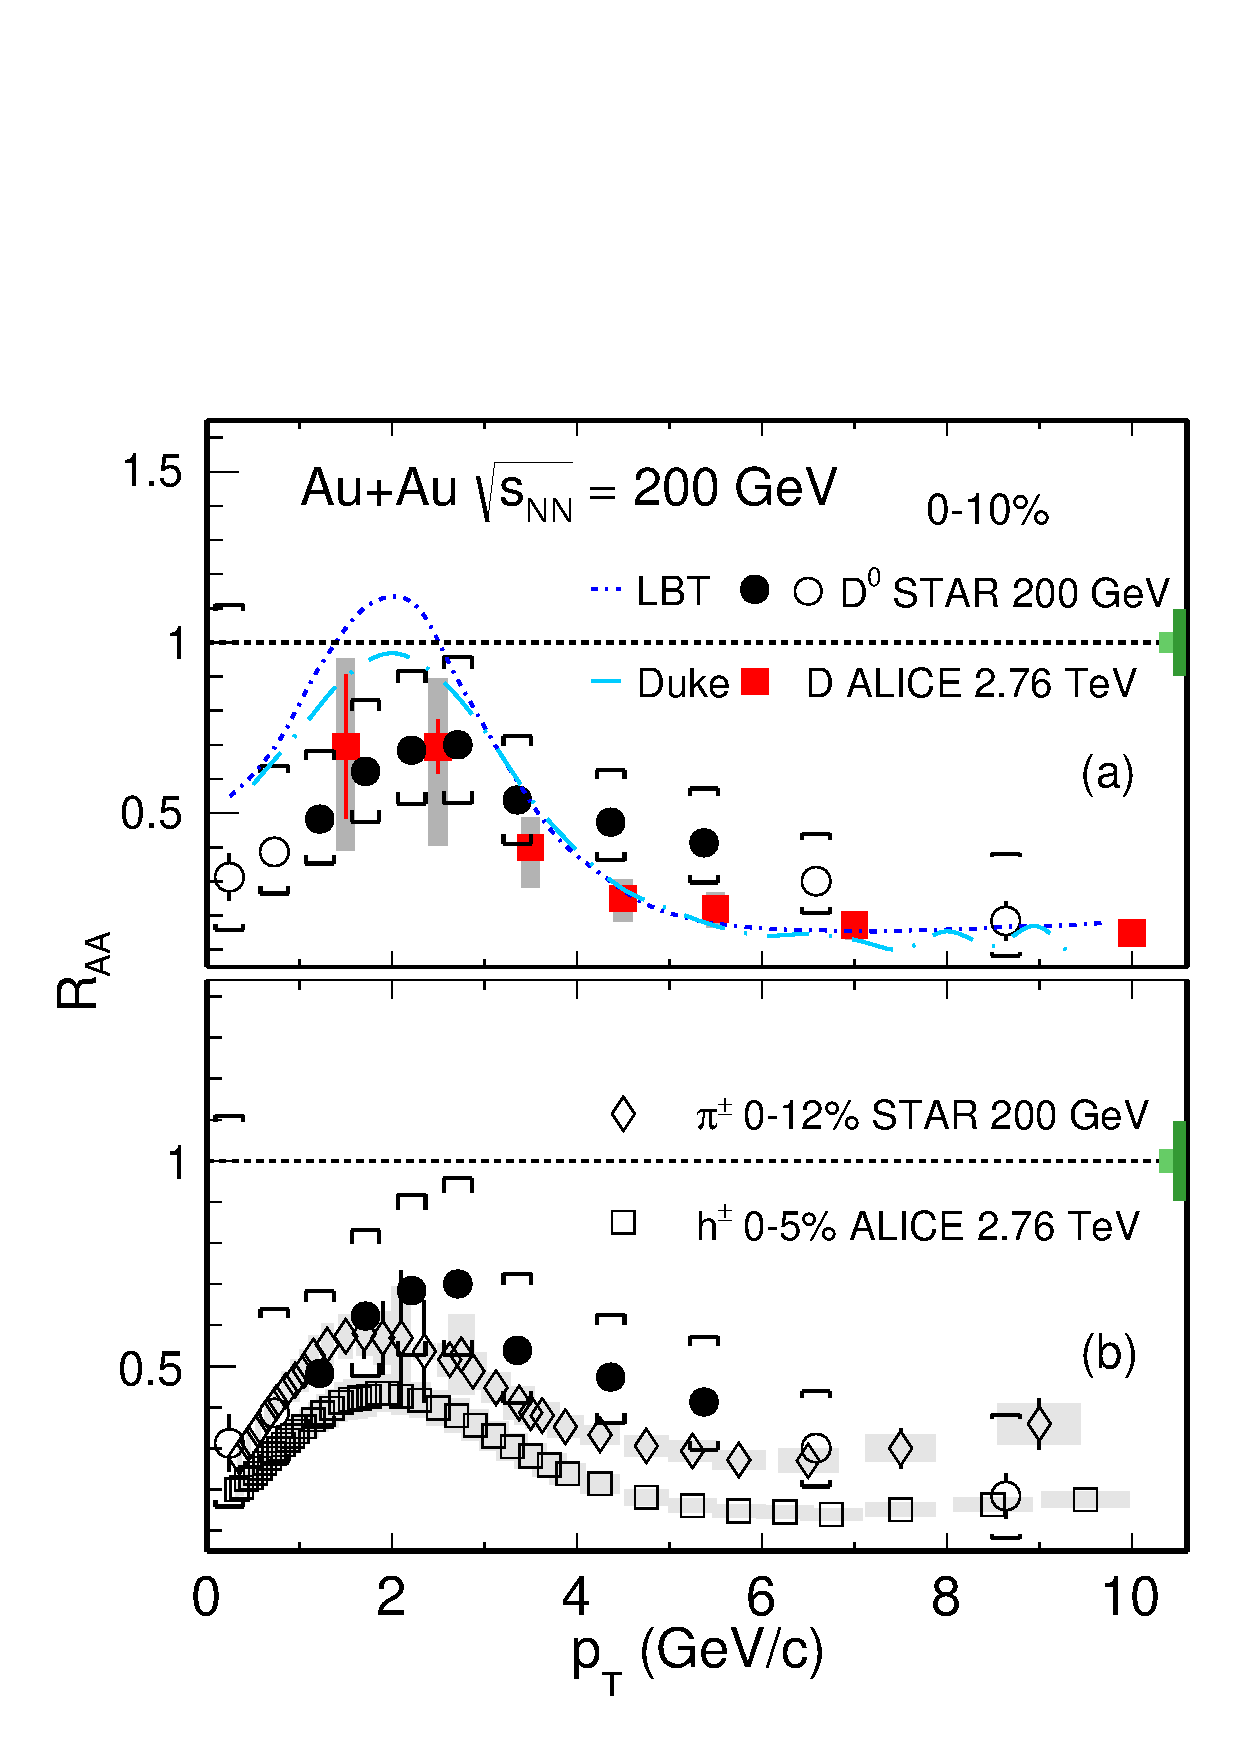
\includegraphics[width=0.45\textwidth]{fig/D0_RAA_LHC.pdf}
\caption{$D^{0}$ $R_{\rm AA}$ in most central ( 0-10\% ) Au + Au collisions at $\sqrt{s_{_{\rm NN}}}$ = 200\,GeV, comparison to ALICE D meson result in most central (0-10\%) Pb + Pb collisions at $\sqrt{s_{_{\rm NN}}}$ = 2.76\,TeV, and hadron from ALICE and $\pi^{\pm}$ from STAR. Also compared to model calculations~\cite{Cao:2016gvr,LBT:private}. The statistical and systematic uncertainties are similar as previous plots.}
\label{fig:D0_RAA_LHC} 
\end{figure}

Figure~\ref{fig:D0_RAA} shows the calculated $R_{\rm AA}$ with the $p+p$ measurement ~\cite{Star_D_pp} as the reference for different centrality bins 0--10\% (a), 10--40\% (b) and 40--80\% (c) and compared with the previous measurements using the STAR TPC after the recent correction~\cite{Star_D_RAA_corr}. The $p+p$ $D^0$ reference spectrum is updated using the latest global analysis of charm fragmentation ratios from~\cite{charm_frag} and also by taking into account the $p_T$ dependence of the fragmentation ratio between $D^0$ and $D^∗_\pm$ from PYTHIA. The new measurement with the HFT detector shows a nice agreement with the measurement without the HFT, but with much improved precision. The grey bands around each data point depict the $p+p$ systematic uncertainty on the measured $D^0$ data points. The first two and last two data points are empty circles indicating those are extrapolated $p+p$ reference. The dark and light green boxes around unity on the right side indicate the global $N_{\rm bin}$ systematic uncertainties for the corresponding centrality bin in each panel and the global cross section uncertainties from $p+p$.

The measured $D^0$ $R_{\rm AA}$ in central (0-10\%) and mid-central (10-40\%) collisions show a significant suppression at the high $p_{\rm T}$ range which reaffirms the strong interactions between charm quarks and the medium, while the new Au+Au data points from this analysis contain much improved precision. Fig.~\ref{fig:D0_RAA_LHC} shows the $D^0$ $R_{\rm AA}$ in the 0-10\% most central collisions compared to that of average D meson from ALICE (a) and charged hadron from ALICE and $\pi^{\pm}$ from STAR (b)~\cite{Alice_D_RAA_2,Alice_hadron_RAA,PhenixPi0}. The comparison of $D^0$ between STAR and ALICE shows reasonable agreement within the uncertainties despite the large energy difference from 200\,GeV to 2.76\,TeV. The comparison to that of light hadrons shows similar suppression at the high $p_{\rm T}$, while in the intermedium range, $D^0$ mesons are less suppressed.



\begin{figure}
\centering
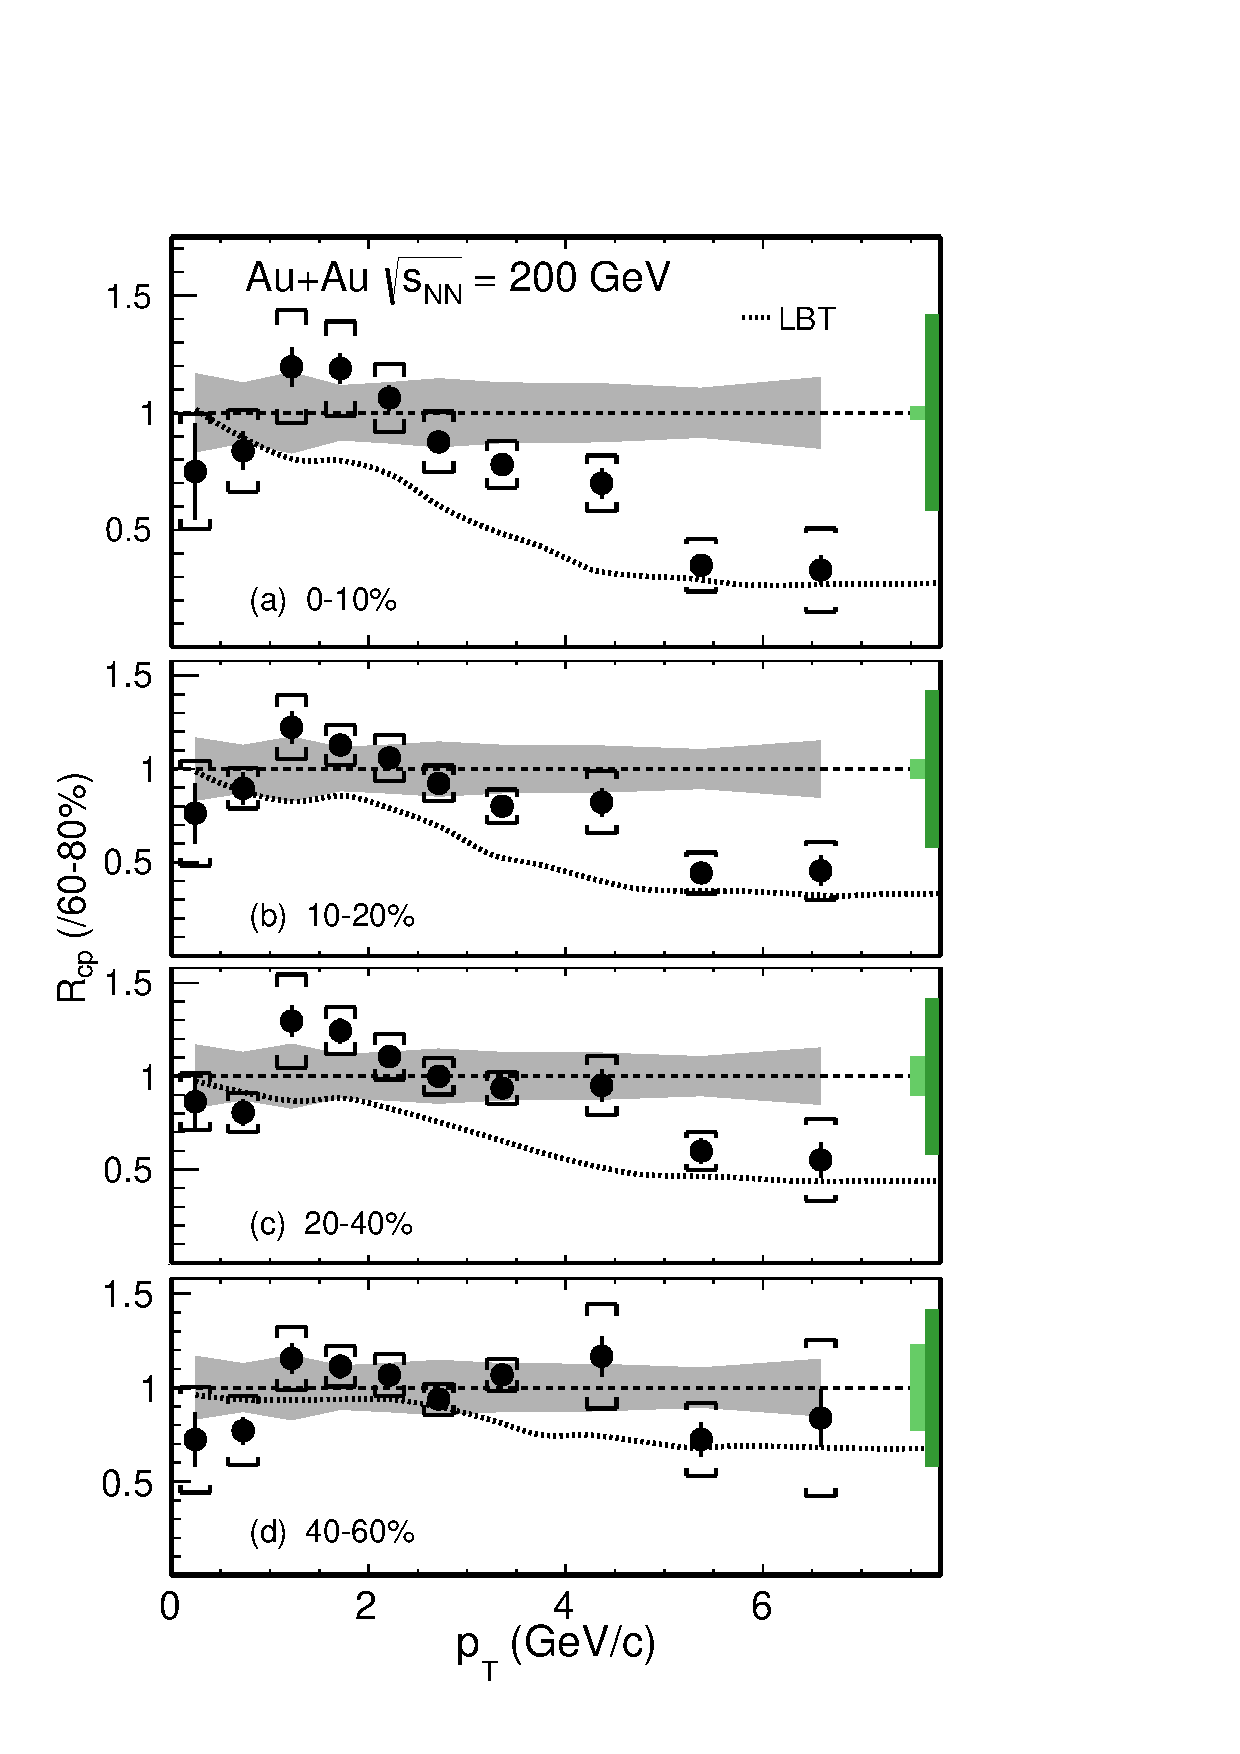
\includegraphics[width=0.45\textwidth]{fig/D0_Rcp11.pdf}
\caption{$D^{0}$ $R_{\rm CP}$ with the 60--80\% spectrum as the reference for different centrality classes in Au + Au collisions compared to model calculations~\cite{Cao:2016gvr,LBT:private}. The statistical and systematic uncertainties are shown as error bars and brackets on the data points. The grey bands around unity depict the systematic uncertainty due to vertex resolution correction, mostly from the 60--80\% reference spectrum. The light and dark green boxes on the right depict the normalization uncertainty in determining the $N_{\rm bin}$.}
\label{fig:D0_Rcp11} 
\end{figure}

\begin{figure}
\centering
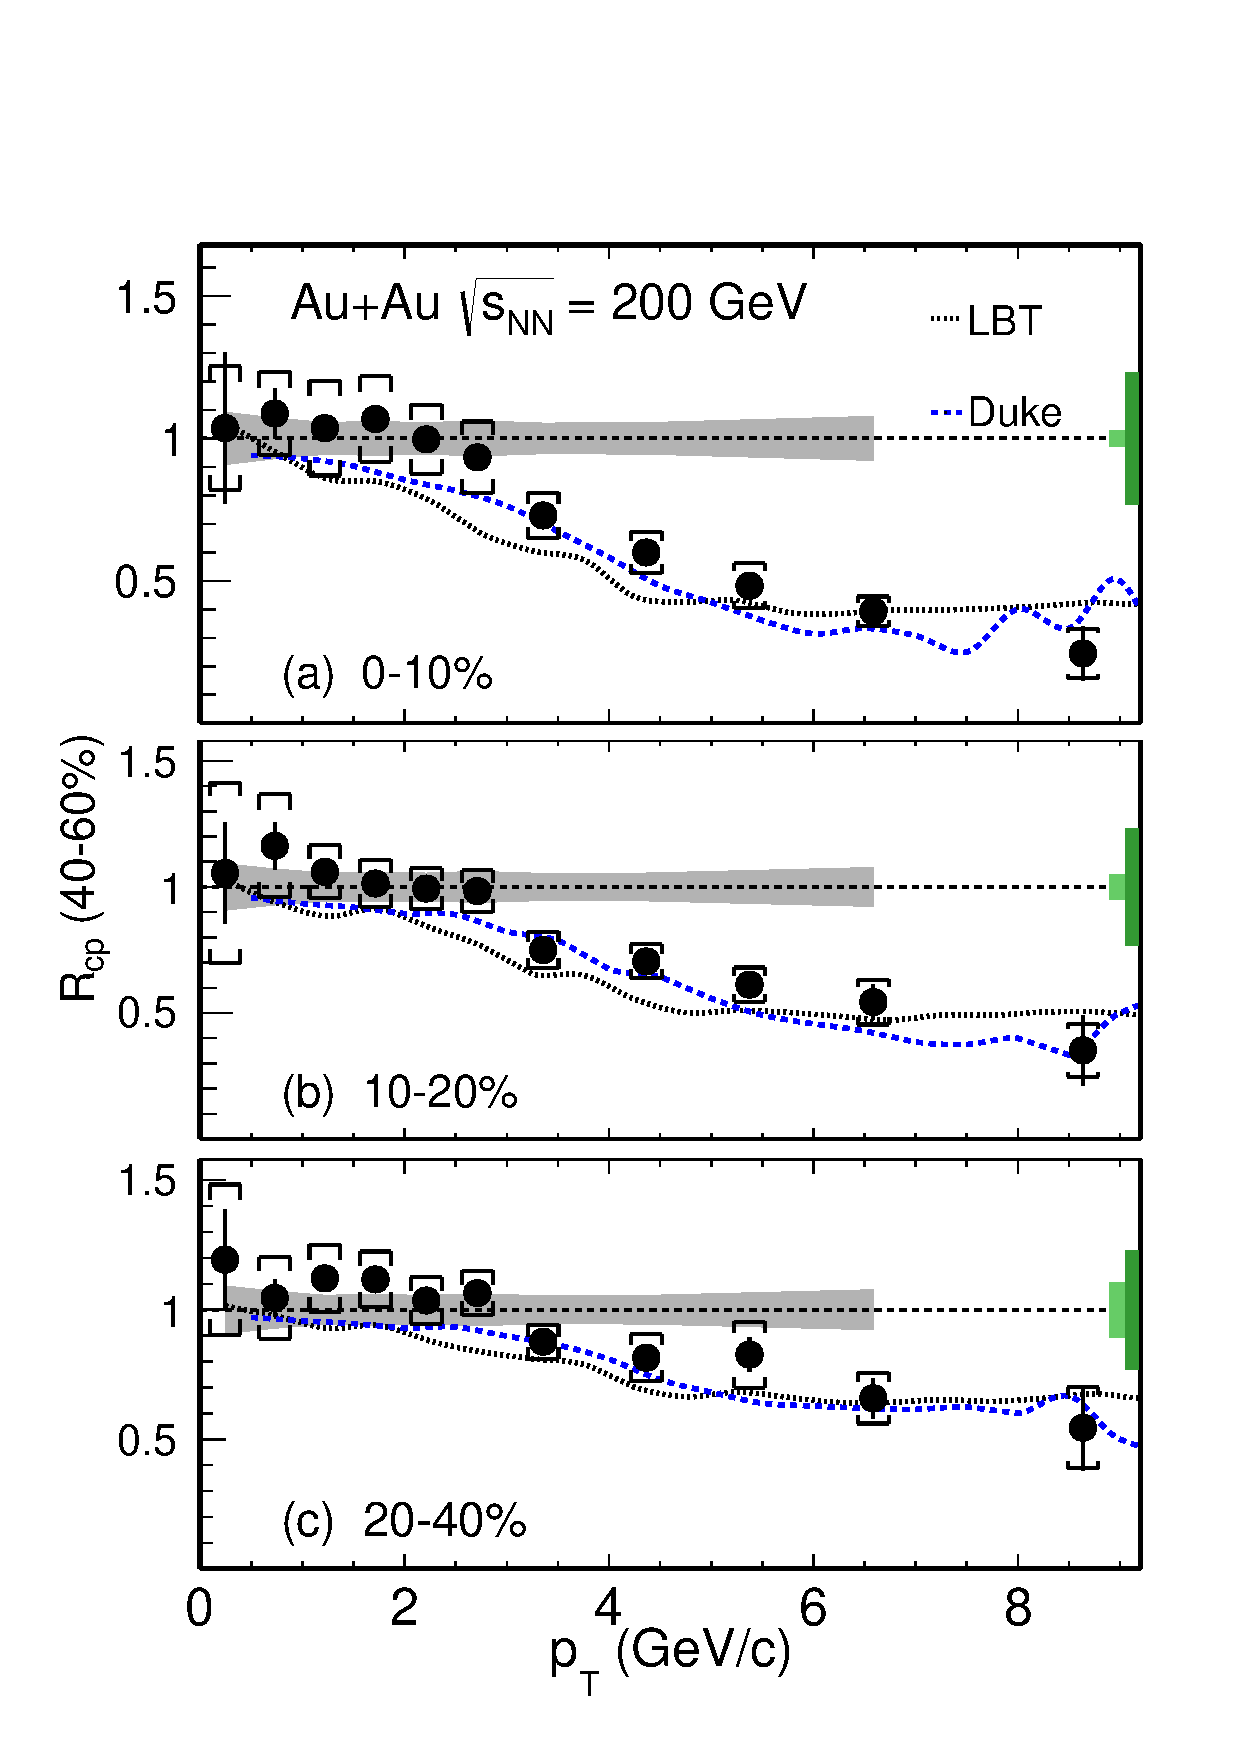
\includegraphics[width=0.45\textwidth]{fig/D0_Rcp22.pdf}
\caption{$D^{0}$ $R_{\rm CP}$ with the 40--60\% spectrum as the reference for different centrality classes in Au + Au collisions compared to model calculations~\cite{Cao:2016gvr,LBT:private,Xu:2017obm}. The statistical and systematic uncertainties are shown as error bars and brackets on the data points. The grey bands around unity depict the systematic uncertainty due to vertex resolution correction, mostly from the 40--60\% reference spectrum. The light and dark green boxes on the right depict the normalization uncertainty in determining the $N_{\rm bin}$.}
\label{fig:D0_Rcp22} 
\end{figure}

% \begin{figure*}
% \centering
% 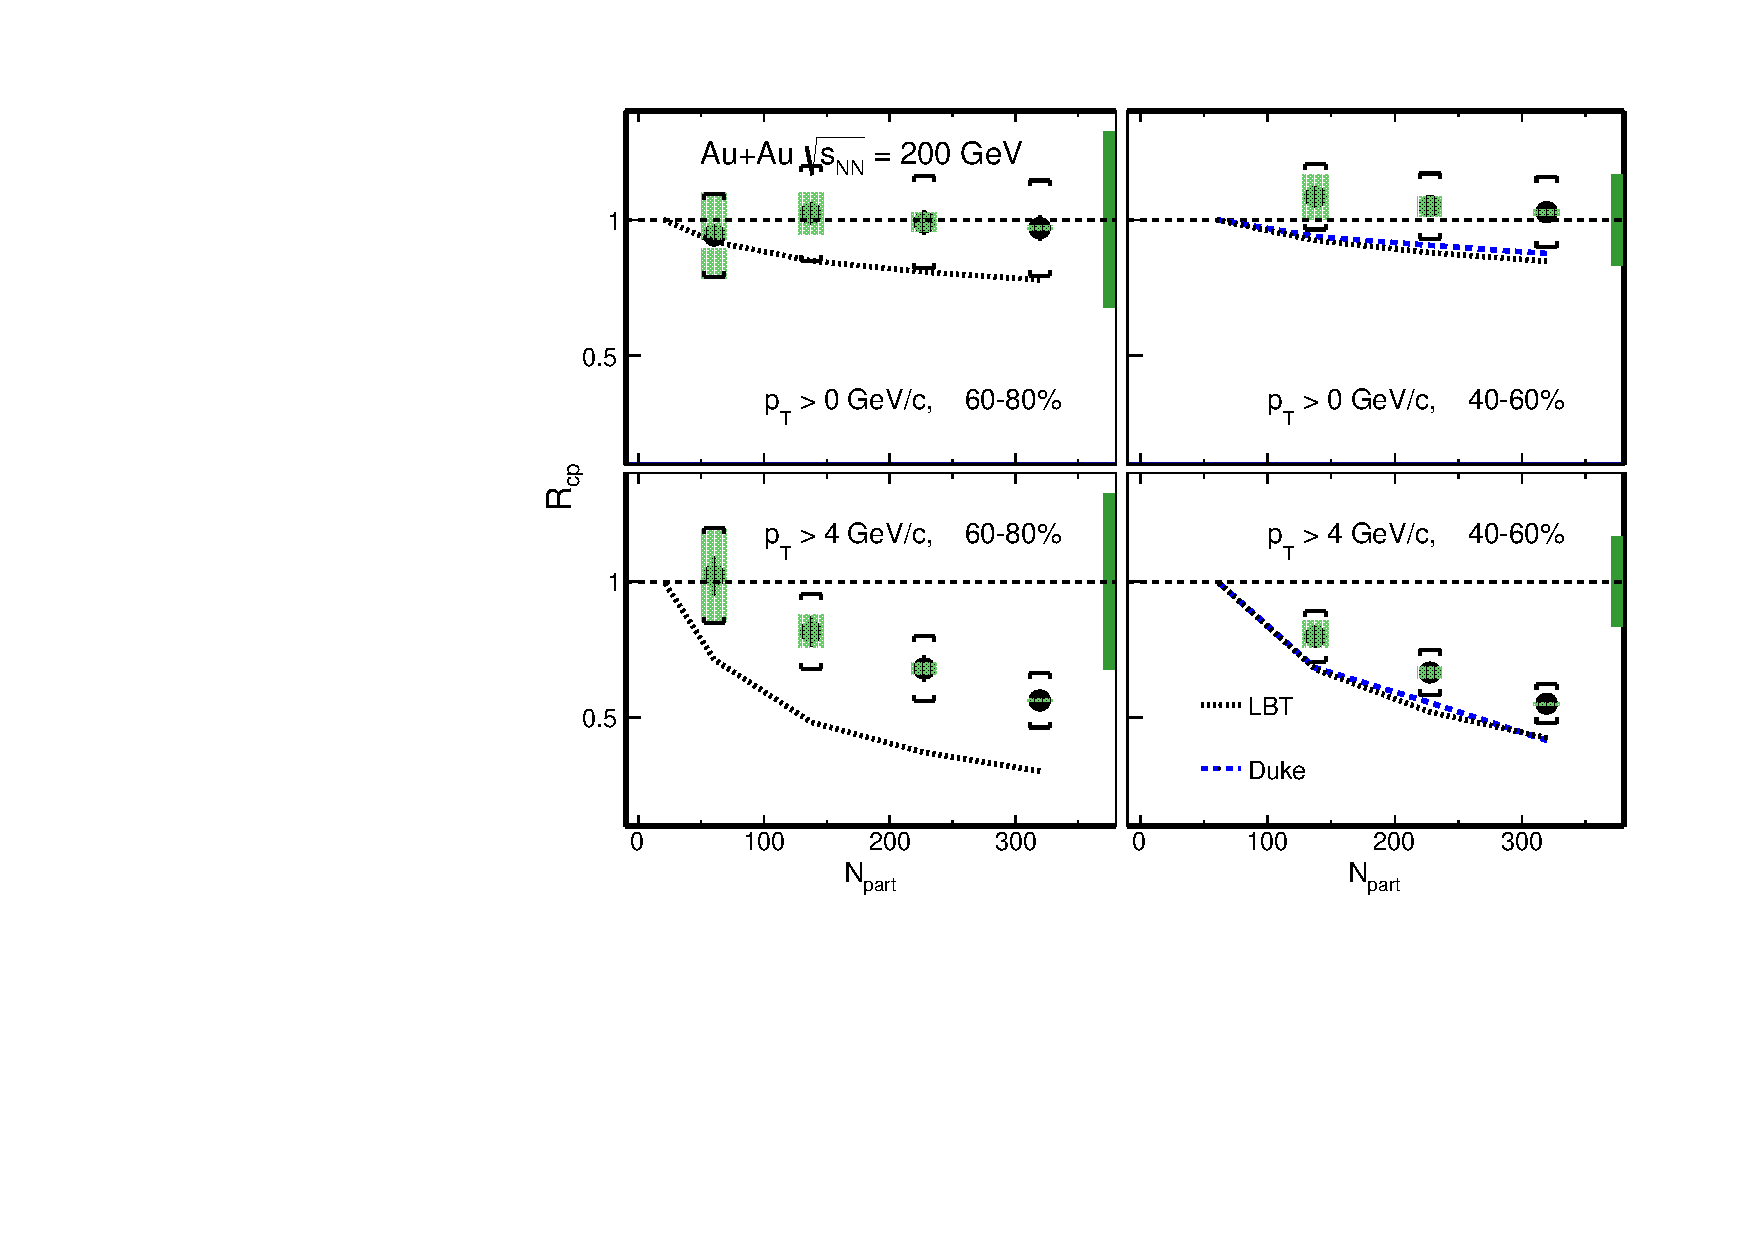
\includegraphics[width=0.8\textwidth]{fig/Rcp_Nbin_D0.pdf}
% \caption{Integrated $D^{0}$ $R_{\rm CP}$ vs. $N_{\rm part}$ for $p_{\rm T}>$ 0\,GeV/$c$ (top) and $p_{\rm T}>$ 4\,GeV/$c$ (bottom), and for 60--80\% reference (left) and 40--60\% reference (right) respectively in Au + Au collisions at $\sqrt{s_{_{\rm NN}}}$ = 200\,GeV. Brackets depict the systematic uncertainties and colored lines represent model calculations from LBT and Duke groups.}
% \label{fig:Rcp_Nbin_D0} 
% \end{figure*}

\subsection{\label{result:D0barD0ratio} $\overline{D}^{0}$ and $D^{0}$ spectra and double ratio}

\begin{figure}
\centering
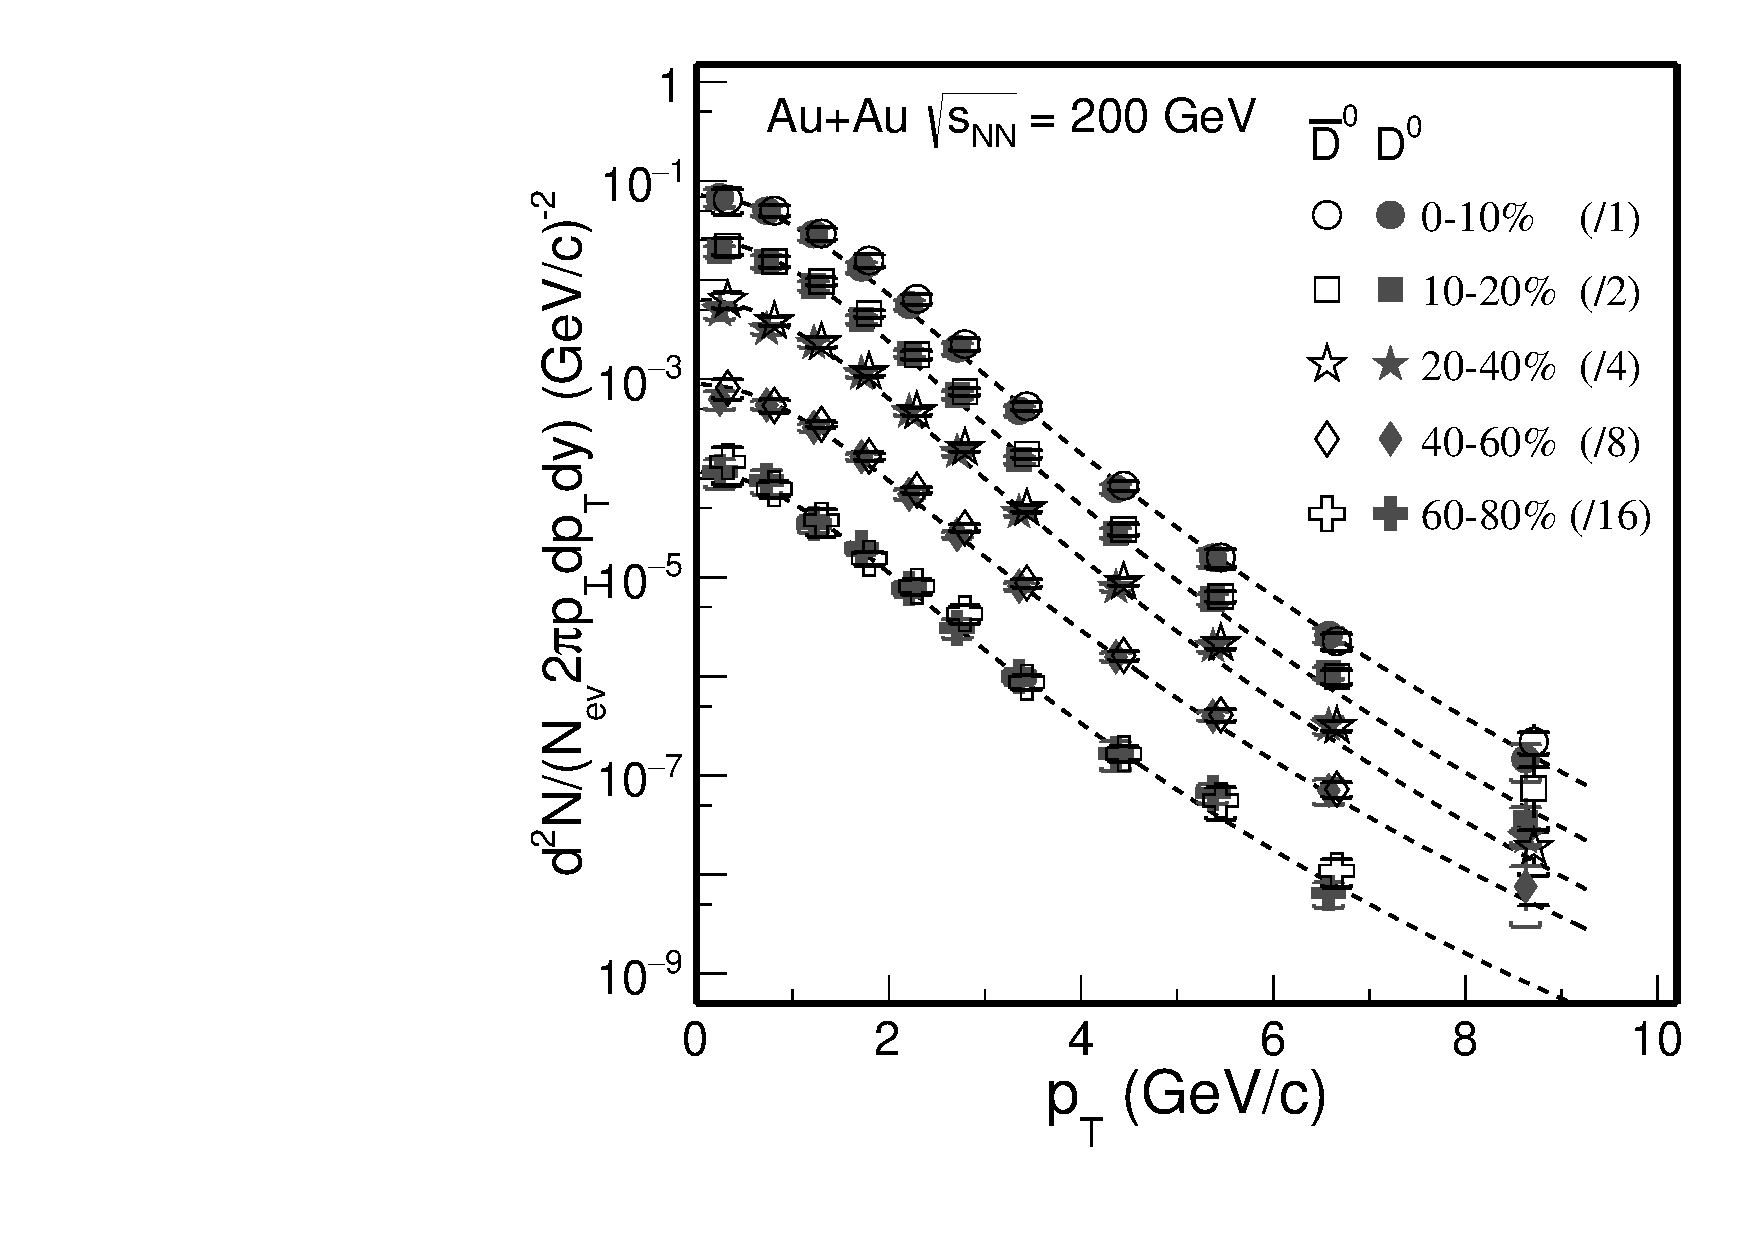
\includegraphics[width=0.45\textwidth]{fig/D0_spectra_bothposneg.pdf}
\caption{$D^{0}$ and $\overline{D}^{0}$ invariant yield at mid-rapidity ($|y|<1$) vs. transverse momentum for different centrality classes in Au + Au collisions at $\sqrt{s_{_{\rm NN}}}$ = 200\,GeV. Error bars (not visible for many data points) indicate statistical uncertainties and brackets depict systematical uncertainties. Global systematic uncertainties in $B.R.$ and $N_{\rm bin}$ are not plotted. Solid lines depict Levy function fits.}
\label{fig:D0_spectra_bothposneg} 
\end{figure}

\begin{figure}
\centering
% 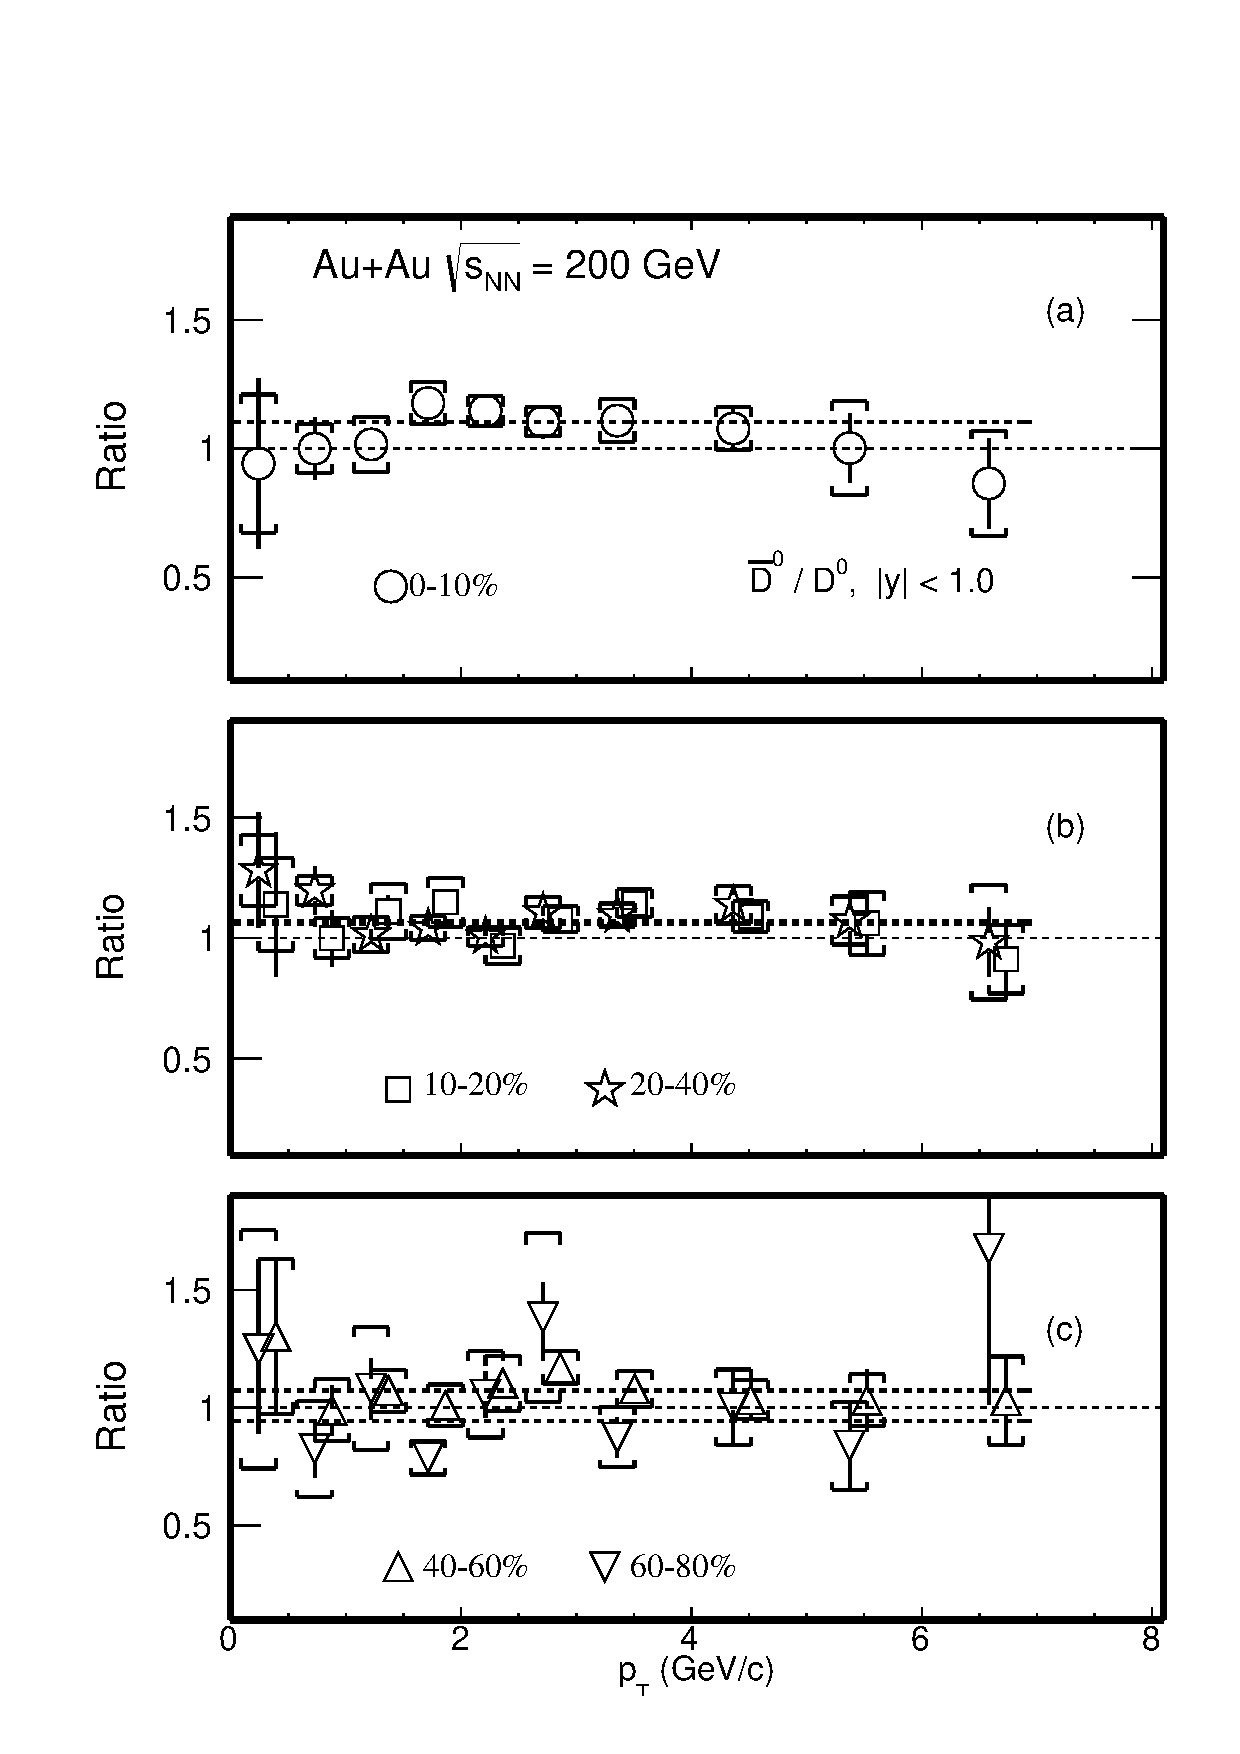
\includegraphics[width=0.45\textwidth]{fig/D0_spectra_ratioposneg.pdf}
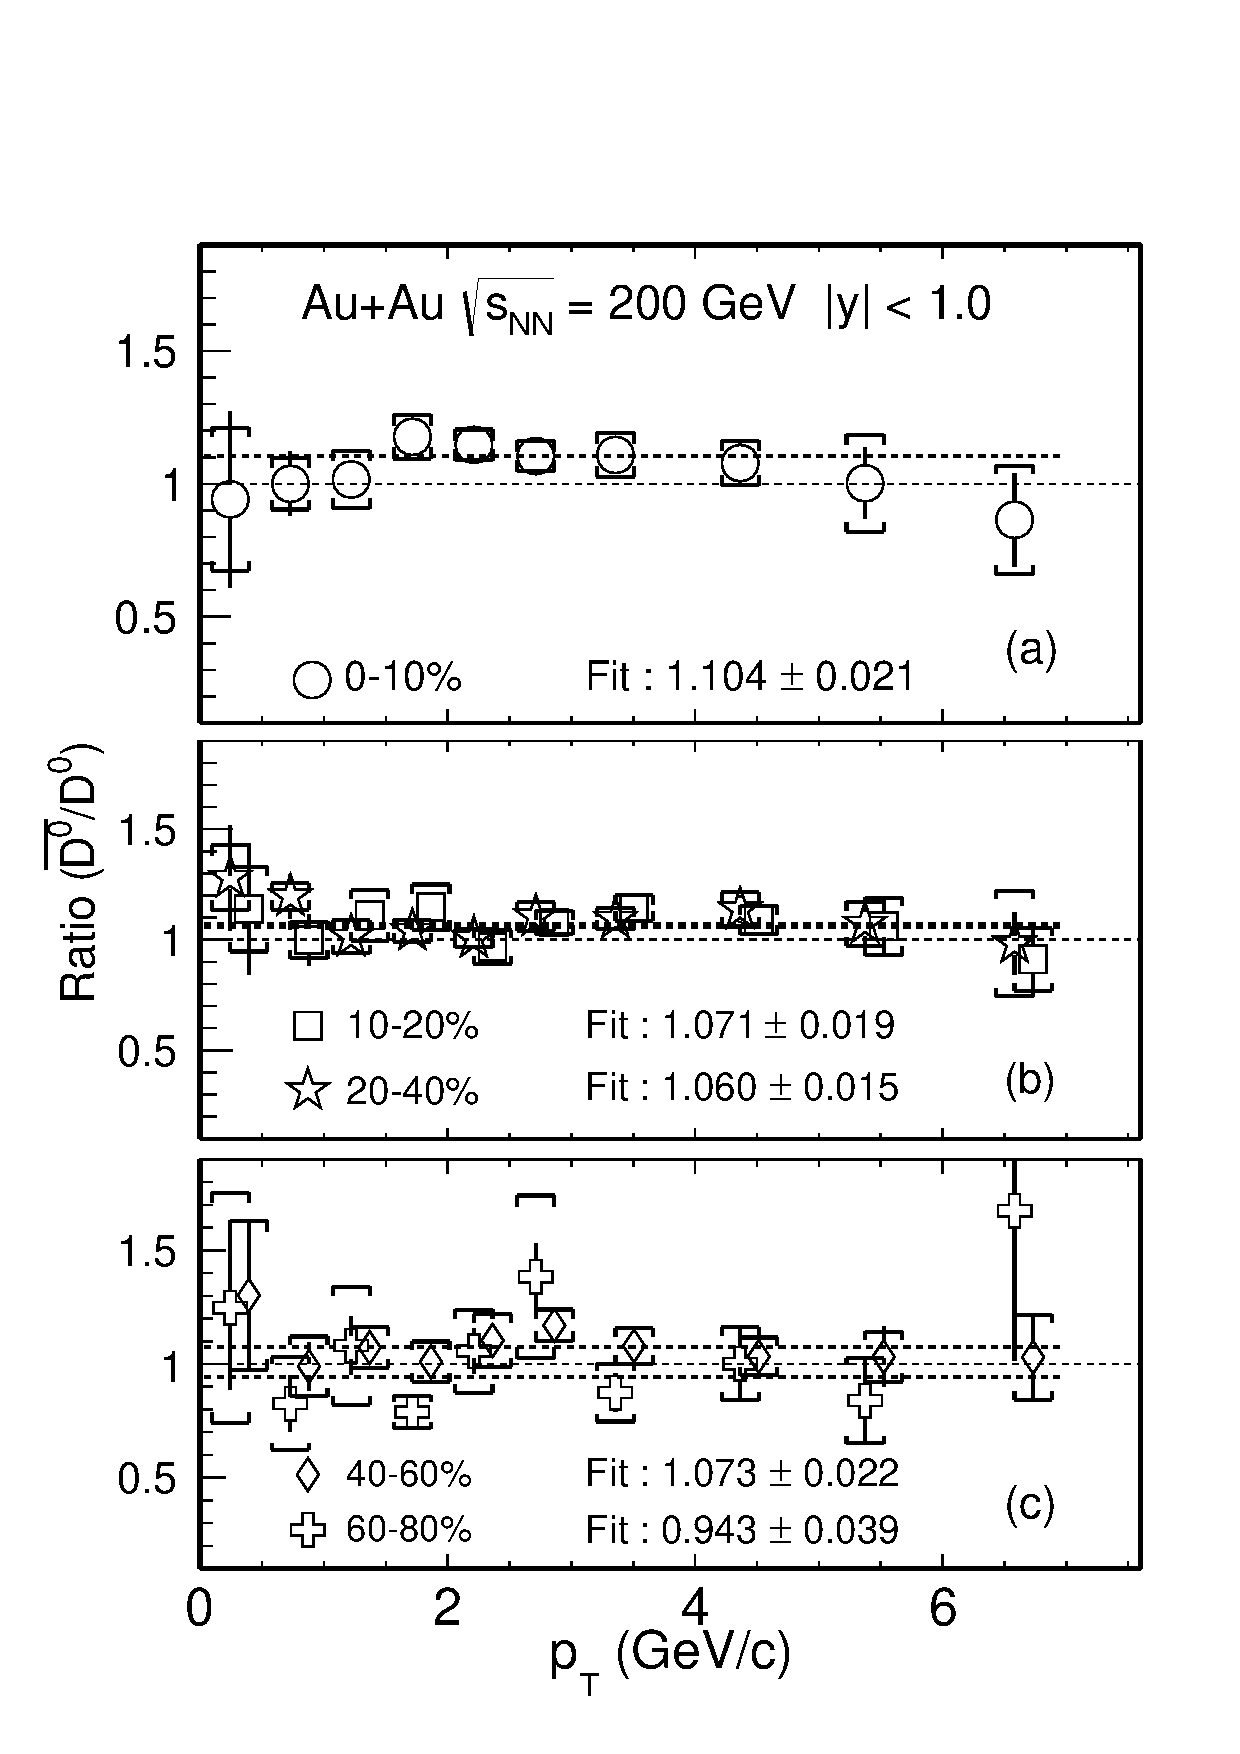
\includegraphics[width=0.45\textwidth]{fig/D0_spectra_ratioposneg_fit.pdf}
\caption{$\overline{D}^{0}$/$D^{0}$ invariant yield ratio at mid-rapidity ($|y|<1$) vs. transverse momentum for different centrality classes in Au + Au collisions at $\sqrt{s_{_{\rm NN}}}$ = 200\,GeV. Error bars indicate statistical uncertainties and brackets depict systematical uncertainties. Dashed lines depict a linear function fits.}
\label{fig:D0_spectra_ratioposneg} 
\end{figure}


Figure~\ref{fig:D0_spectra_bothposneg} shows the $p_{\rm T}$ spectra comparison between $\overline{D}^{0}$ and $D^0$ in 0--10\%, 10--20\%, 20--40\%, 40--60\% and 40--80\% centrality bins. Fig.~\ref{fig:D0_spectra_ratioposneg} shows the $\overline{D}^{0}$/$D^{0}$ ratio in the corresponding centrality bins. With the current data, the $\overline{D}^{0}$ yield is significantly larger than the $D^{0}$ in the most central and mid-central collisions. With the consideration of the statistical and systematic uncertainties, a linear fit is performed to quantify the deviation from unity. Table %~\ref{table:d0bard0ratio}%
VII lists the fitted results for the $\overline{D}^{0}$/$D^0$ ratio from various centralities. In the most central collisions, $\overline{D}^{0}$ yield is higher than the $D^0$ yield by $\sim$4.9$\sigma$ on average. This can potentially be explained by the finite baryon density of the system, from which we expect the $\Lambda_{c}^-$/$\Lambda_{c}^+$ ratio to be smaller than unity. The total charm quark and anti-charm quark should be conserved since they are created in pairs, which results in larger $\overline{D}^{0}$ yield than the $D^0$. This calls for the precise measurement of $D^{+}$/$D^{-}$ and $D_{s}^{+}$/$D_{s}^{-}$ in the future.

\begin{table}[t]
\centering{
  \caption{ $\overline{D}^{0}$/$D^0$ ratio for various centrality bins obtained from the fit to data distributions in Fig.~\ref{fig:D0_spectra_ratioposneg}.}
\begin{tabular}{rcccccccc} \hline \hline
  \hspace{1cm}Centrality\hspace{1cm} & \multicolumn{3}{c}{$\overline{D}^0$/$D^0$} & \hspace{1cm} \\ \hline
0--10 \%\hspace{1cm}      & 1.104 & $\pm$ & 0.021 \\
10--20 \%\hspace{1cm}     & 1.071 & $\pm$ & 0.019 \\
20--40 \%\hspace{1cm}     & 1.060 & $\pm$ & 0.015 \\
40--60 \%\hspace{1cm}     & 1.073 & $\pm$ & 0.022 \\
60--80 \%\hspace{1cm}     & 0.943 & $\pm$ & 0.039  \\ \hline \hline
\end{tabular}
}
\label{table:d0bard0ratio}
\end{table}

% \begin{figure*}
% \centering
% \includegraphics[width=0.45\textwidth]{fig/Teff_mb.pdf}
% \caption{Slope parameters $T_{eff}$ versus invariant mass for different particles.}
% \label{fig:Teff_mb} 
% \end{figure*}

% Figure~\ref{fig:Teff_mb} shows the slope parameters $T_{eff}$ in the transverse mass spectrum for different particles.


\subsection{\label{result:theory}Comparison to Models}

Over the past several years, there have been rapid developments in the theoretical calculations on the charm hadron production. Here we compare our measurements to several recent calculations based on the Duke model and the Linearized Boltzmann Transport (LBT) model.

The Duke model~\cite{Duke,Xu:2017obm,DukePrivateCom} uses a Langevin stochastic simulation to trace the charm quark propagation inside the QGP medium. Both collisional and radiative energy losses are included in the calculation and charm quarks are hadronized via a hybrid approach combining both coalescence and fragmentation mechanisms. The bulk medium is simulated using a viscous hydrodynamic evolution and a hadronic cascade evolution using the UrQMD model~\cite{urQMD}. The charm quark interaction with the medium is characterized using a temperature and momentum-dependent diffusion coefficient. The medium parameters have been constrained via a statistical Bayesian analysis by fitting the previous experimental data of $R_{\rm AA}$ and $v_{2}$ of light, strange and charm hadrons~\cite{Xu:2017obm}. The extracted charm quark spatial diffusion coefficient at zero momentum $2\pi TD_s|_{p=0}$ is about 1--3 near $T_{\rm c}$ and exhibits a positive slope for its temperature dependence above $T_{\rm c}$.

The Linearized Boltzmann Transport (LBT) calculation~\cite{Cao:2016gvr} extends the LBT approach developed before to include both light and heavy flavor parton evolution in the QGP medium. The transport calculation includes all $2\rightarrow 2$ elastic scattering processes for collisional energy loss and the higher-twist formalism for medium induced radiative energy loss. It uses the same hybrid approach as in the Duke model for charm quark hadronization. The heavy quark transport is coupled with a 3D viscous hydrodynamic evolution which is tuned for light flavor hadron data. The charm quark spatial diffusion coefficient is estimated via the $2\pi TD_s =8\pi/\hat{q}$ ($\hat{q}$, is the quark transport coefficient due to elastic scatterings) at parton momentum $p = 10$\,GeV/$c$. The $2\pi TD_s$ is $\sim$3 at $T_{\rm c}$ and increases to $\sim$6 at $T = 500$\,MeV~\cite{LBT:private}.

Figure~\ref{fig:D0_Rcp11} and ~\ref{fig:D0_Rcp22} show the measured $D^0$ $R_{\rm CP}$ compared to the Duke and LBT model calculations with the 60--80\% and 40--60\% reference spectra respectively. The $R_{\rm CP}$ curves from these models are calculated based on the $D^0$ spectra provided by each group~\cite{Cao:2016gvr,LBT:private,Xu:2017obm}. The Duke model did not calculate the spectra in the 60--80\% centrality bin due to the limitation of the viscous hydrodynamic implementation. In the Fig.~\ref{fig:D0_RAA_LHC} for the most central collisions, there are also calculations for the $D^0$ $R_{\rm AA}$ from the Duke and LBT group respectively. These two models also have the prediction for the $D^0$ $v_2$ measurements for Au + Au collisions at $\sqrt{s_{_{\rm NN}}}$ = 200\,GeV~\cite{Star_D_v2}. %One note is that both models have been tuned to reproduce our previously published $D^0$ $R_{\rm AA}$ results at $p_{\rm T}>$ 2\,GeV/$c$~\cite{Star_D_RAA} while have some discrepancy with the new measured $R_{\rm AA}$. It is not surprising to see that the tuned calculation match to our new measured $R_{\rm CP}$ data points well. However, the much improved precision of these new measurements are expected to further constrain the theoretical model uncertainties in these calculations.
Both model calculation match to our new measured $R_{\rm CP}$ data points well. However, the much improved precision of these new measurements are expected to further constrain the theoretical model uncertainties in these calculations.

% Figure~\ref{fig:Rcp_Nbin_D0} shows the $p_{\rm T}$ integrated $R_{\rm CP}$ compared to the model calculations for two different integration regions.

% Chapter five
\section{\label{summary}Summary}

In summary, we report the improved measurement of $D^0$ production yield in Au + Au collisions at $\sqrt{s_{_{\rm NN}}}$ = 200\,GeV with the STAR HFT detector. $D^0$ invariant yields are presented as a function of $p_{\rm T}$ in various centrality classes. There is a hint (1.5 $\sigma$) that the $p_{\rm T}$ integrated $D^0$ yields at mid-rapidity in mid-central and central Au+Au collisions are smaller than that measured in $p+p$ collisions, indicating that cold nuclear matter (CNM) effects and/or charm quark coalescence hadronization may play an important role in Au+Au collisions. This calls for precise measurements of $D^0$ production in $p/d$+A collisions to understand the CNM effects as well as other charm hadron states in heavy-ion collisions to better constrain the total charm quark yield.

The $D^0$ spectra at low $p_{\rm T}$ and low $m_{\rm T}$ are fit to the exponential function and the Blast-Wave model to study the radial collectivity. The slope parameter extracted from the exponential function fit for $D^0$ mesons follow the same linear increasing trend vs. particle mass as $\phi,\Lambda,\Xi^-,\Omega^-$ particles, but different from the trend of $\pi,K,p$ particles. The extracted kinetic freeze-out temperature and transverse velocity from the Blast-Wave model fit are comparable to the fit results of $\phi,\Xi^-$ multi-strange hadrons, but different from those of $\pi,K,p$. These suggest that $D^0$ hadrons show a radial collective behavior with the medium, but freeze out from the system earlier and gain less radial collectivity compared to $\pi,K,p$ particles. This observation is consistent with collective behavior observed in $v_2$ measurements. The fit results also suggest that $D^0$ mesons have similar kinetic freeze-out properties as multi-strange hadrons $\phi,\Xi^-$.

Nuclear modification factors $R_{\rm CP}$ of $D^0$ mesons are presented with both 60--80\% and 40--60\% centrality spectra as the reference, respectively. The $D^0$ $R_{\rm CP}$ is significantly suppressed at high $p_{\rm T}$ and the suppression level is comparable to that of light hadrons at $p_{\rm T}>$ 5\,GeV/$c$, re-affirming our previous observation. This indicates that charm quarks lose significant energy when traversing through the hot QCD medium. The $D^0$ $R_{\rm CP}$ is above the light hadron $R_{\rm CP}$ at low $p_{\rm T}$. We compare our $D^0$ $R_{\rm CP}$ measurements to two recent theoretical model calculations. The models show nice agreements to our new $R_{\rm CP}$ measurements. We expect the new data points with much improved precision can be used in the future to further constrain our understanding of the charm-medium interactions as well as to better determine the medium transport parameter.

% Chapter acknowledgement
\section{\label{acknowledgement}Acknowledgement}

We thank the RHIC Operations Group and RCF at BNL, the NERSC Center at LBNL, and the Open Science Grid consortium for providing resources and support. This work is supported in part by the Office of Nuclear Physics within the U.S. DOE Office of Science, the U.S. National Science Foundation, the Ministry of Education and Science of the Russian Federation, National Natural Science Foundation of China, Chinese Academy of Science, the Ministry of Science and Technology of China and the Chinese Ministry of Education, the National Research Foundation of Korea, GA and MSMT of the Czech Republic, Department of Atomic Energy and Department of Science and Technology of the Government of India; the National Science Centre of Poland, National Research Foundation, the Ministry of Science, Education and Sports of the Republic of Croatia, RosAtom of Russia and German Bundesministerium fur Bildung, Wissenschaft, Forschung and Technologie (BMBF) and the Helmholtz Association.

\bibliography{D0spectra}

\end{document}
%
% ****** End of file apssamp.tex ******
